\documentclass[11pt]{book}

\usepackage{jyw-program-book}

\begin{document}

%----------------------------------------------------------------------------------------
%	TITLE PAGE
%----------------------------------------------------------------------------------------

\begingroup
\thispagestyle{empty}
\begin{tikzpicture}[remember picture,overlay]
\node[inner sep=0pt] (background) at (current page.center) {\includegraphics[width=\paperwidth]{background}};
\draw (current page.center) node [fill=ocre!30!white,fill opacity=0.6,text opacity=1,inner sep=1cm]{\Huge\centering\bfseries\heiti\parbox[c][][t]{\paperwidth}{\centering C/\cc{} 程式語言講義\\[15pt]\songti % Book title
{\LARGE 瘋狂程設題解}\\[20pt] % Subtitle
%{\LARGE 王佳盈}}}; % Author name
{\LARGE 王佳盈\\ \Large
梁家萁、侯怡安、朱睿謙、巫鈺瑩、周身鴻}}}; % Author name
\end{tikzpicture}
\vfill
\endgroup

%----------------------------------------------------------------------------------------
%	COPYRIGHT PAGE
%----------------------------------------------------------------------------------------

\newpage
~\vfill
\thispagestyle{empty}

\noindent Copyright \copyright\ 2017 Jia-Yin Wang\\ % Copyright notice

\noindent \textsc{中原電機CTRL 501實驗室}\\ % Publisher

\noindent \textsc{jywglady@gmail.com}\\ % URL

\noindent 本書版權屬中原大學電機系CTRL實驗室所有。未經事前書面授權,不得以任何方式(包括儲存於資料庫或任何存取系統內)作全部或局部之翻印、仿製或轉載。書內圖片及資料來源已盡查明之責,若有疏漏致版權遭侵犯,我們在此致歉,並請有關人士致函本實驗室,我們將作最適當的修訂和安排。\\ % License information

\noindent \textit{2017年十月,第一版} % Printing/edition date

%----------------------------------------------------------------------------------------
%	TABLE OF CONTENTS
%----------------------------------------------------------------------------------------

%\usechapterimagefalse % If you don't want to include a chapter image, use this to toggle images off - it can be enabled later with \usechapterimagetrue

\chapterimage{chapter_head_1.pdf} % Table of contents heading image

\pagestyle{empty} % No headers
\setcounter{tocdepth}{1}
\tableofcontents % Print the table of contents itself

\cleardoublepage % Forces the first chapter to start on an odd page so it's on the right

\pagestyle{fancy} % Print headers again



%\begin{abstract}
%\frontmatter

%\maketitle

%\tableofcontents

\part{行前準備}
\chapter{前言}
我喜歡寫程式,寫程式可以說是學習和電腦打交道的過程。在寫程式的過程中,會發現電腦可以說得上是一位忠實、公正,又極有耐心的朋友,這些特質電腦發揮得極其盡緻,世間的朋友很難比得上。首先它非常客觀公正,無論情況多麼撲朔迷離,它仍然會在其中依循既定的原則而行,絕沒有一絲一豪偏離軌道;也不管你的程式功力多麼高深,程式寫得多麼巨大華麗,對於那豪不起眼的一點小小錯誤,它也絕不會輕易地把你放過,這是它忠實、公正的特質。另外,不管你的程式能力多麼拙劣,永無止盡的在相同的小錯誤中周旋,它也絕不失去耐心,乃至發出一點點怒火,仍然保持著冷靜沈著,一再地把最忠實而相同的錯誤訊息反應給你,這樣的耐心幾乎無人能及。如果要說它的一些缺點,大概就是有點不盡人情,有時候迂腐得可以。

寫程式跟學習世間的技能,過程非常一致。一個人學習游泳,學習騎腳踏車,如果沒有真正下水或上路練習,而只是詳細閱讀教學手冊,要真正在水中得到游泳的樂趣,或者在路上騎乘的快感,那幾乎是不太可能的事。同樣地,一個學習寫程式的人,如果沒有真正上機練習,而光是閱讀程式教學的書籍,要真正具備寫作程式的能力,那也是非常困難的事情。初學游泳的人,總是要在水中嗆幾口水;初學騎腳踏車的人,也不免有不穩或摔倒的時候,這都是學習過程普遍發生的事情。相同地,初學程式的人,總會有弄不清頭緒,在不解的錯誤中周旋的時候,這是一種除錯和學習的過程,不用因此而灰心喪志,只要持續努力,慢慢會掌握寫程式的一些絕竅。

我因為喜歡寫程式,後來也有機會開始擔任C/\cc{}程式的教學。因為了解學習程式必須實際練習,所以也一直在尋找合適的學習資源。現在網路非常發達,資訊詳盡而多元,要找到一些學習資源並不太難,但是在尋找C/\cc{}的學習資源的過程中,發現大部份的學習工具和平台多是英語介面,對於國內很多學生來說,還是有一些不容易跨越的門檻。後來在尋覓的過程中,發現了銘傳大學謝育平老師所寫作的「瘋狂程設」,這個平台不僅完全使用中文,而且還可以把許多教學、作業和解題的過程融合在一個系統中,不僅對初學程式的人極有幫助,對於程式教學的老師來說,也提供非常有用的資源,可以達到事半功倍的效果。後來也承蒙謝老師的幫助,連續幾年開課,我都一直使用這個學習平台,作為教學的輔助資源。

「瘋狂程設」的平台中,提供了很多練習題目,可以讓學習程式的人練習,而老師也可以使用這個系統,不斷開發新的題目。對於剛入門的同學來說,「瘋狂程設」有一個程式練習廣場,裡面很有系統地提供一些基礎的題目,讓初學的人練習解題,漸次深入,這就好像玩遊戲過關斬將一樣,讓學習程式也可以變得很有樂趣。對於老手來說,這些題目可能不堪一擊,但對初學者來說,很多人經常卡關,面對題目不知所措,甚至充滿了挫折。這本書的內容,主要就是針對程式練習廣場的題目,提供詳盡的思惟過程和解題參考,可以作為初學者的破關攻略,也可以從中看到各種不同的解題技巧。

這本書能夠完成,還要特別感謝實驗室幾位研究生,包括梁家萁、侯怡安、朱睿謙、巫鈺瑩、以及周身鴻等人。我讓他們每個人先練習撰寫書中的一小部份章節,一方面他們可以練習,一方面我也可以減輕一些負擔,等他們寫完各章節之後,我再整體看過並做修改。所以這本書能夠完成,也要非常感謝這些同學的幫忙。

我希望這本書可以幫助到初學C/\cc{}程式的人,也希望提供給程式教學的老師作為教學的參考,減輕彼此教和學的負擔和困難,乃至達到事半功倍的效果。書中的內容,主要針對問題如何思考和解答來做說明,所以不是完整的教科書,很多C/\cc{}語言基本的概念,還是應該要參閱其他的書籍和資源。

另外,寫程式要有相對應的開發工具,在教學上,我習慣使用的整合開發環境是Code::Blocks,這是一套跨平台的自由軟體,功能實用而且豐富;而編譯程式用的編譯器則是使用mingw,這是gcc移植到Windows的版本,也可以說是非常普及而強大的編譯工具。讀者只要連到Code::Blocks的官網,可以直接下載內含mingw的Code::Blocks版本,非常便利。本書第一部份也會針對Code::Blocks的安裝以及瘋狂程設的使用做一些說明。

我必須再次強調,學習程式一定要自己思考和練習,如果只是光看而不練的話,實際遇到問題,還是做不出來的。因此同學在使用本書的時候,除了閱讀之外,也要花一些時間自己思考,並且實際上機練習解題,務求每一個步驟都充份了解和熟悉,這樣才能達到理想的功效。

對於本書的內容,如果有什麼修正建議或錯誤指正,還請不吝提供給我們作為修正的參考,連絡方式,可以寄信到\ \href{mailto:jywglady@gmail.com}{jywglady@gmail.com}\ 電子信箱,我們先在此感謝您的幫忙。最後敬祝大家學習愉快,一切平安吉祥。

\begin{flushright}
	王佳盈 寫於 2018/06
\end{flushright}

%\end{abstract}

%\setcounter{tocdepth}{2}
%\tableofcontents
\mainmatter
\chapter{安裝與設定}

工欲善其事,必先利其器。在學習程式語言之前,也要先設定好程式的學習環境。這一章會教同學如何安裝及設定本書所使用的學習環境,首先說明如何安裝「Code::Blocks」以及「瘋狂程設」;其次,說明如何註冊瘋狂程設的帳號,並針對開課及修課的需要,說明如何在瘋狂程設中加選課程;最後,簡單介紹如何使用瘋狂程設解題。

\section{安裝CodeBlocks}
%\subsection{步驟一:下載}
	在Google搜尋輸入關鍵字「codeblocks」,選擇搜尋結果「Download binary - Code::Blocks」。也可以直接輸入以下網址 \url{http://www.codeblocks.org/downloads/26},參考\autoref{install001}。

	進入官網下載頁面後,選擇包含mingw-setup的檔案,點選該檔案右邊的連結下載,參考\autoref{install002}。

	\begin{figure}[H]
		\centering
		\includegraphics[width=0.8\textwidth]{fig/install_and_setting/install_001_searchCodeblocks}
		\caption{codeblocks搜尋結果}
		\label{install001}
	\end{figure}

	\begin{figure}[H]
		\centering
		\includegraphics[width=0.8\textwidth]{fig/install_and_setting/install_002_Download_binary}
		\caption{Download binary頁面}
		\label{install002}
	\end{figure}
	
	找到剛剛下載的安裝檔codeblocks-16.01mingw-setup.exe,點兩下開啟安裝精靈,參考\autoref{install003}。
	\begin{figure}[H]
		\centering
		\includegraphics[width=0.8\textwidth]{fig/install_and_setting/install_003_openEXE}
		\caption{點兩下開啟CodeBlocks安裝檔}
		\label{install003}
	\end{figure}
	
	請不要修改安裝精靈的任何設定,只要一直點「Next」就好。絕對不可以更改檔案路徑,參考\autoref{install004}。
		\begin{figure}[H]
			\centering
			\includegraphics[width=0.8\textwidth]{fig/install_and_setting/install_004_setup01}
			\caption{啟動安裝精靈,點「Next」}
			\label{install004}
		\end{figure}
	
		\begin{figure}[H]
			\centering
			\includegraphics[width=0.8\textwidth]{fig/install_and_setting/install_005_setup02}
			\caption{點「I Agree」}
		\end{figure}
			
		\begin{figure}[H]
			\centering
			\includegraphics[width=0.8\textwidth]{fig/install_and_setting/install_006_setup03}
			\caption{全部打勾,點「Next」}
		\end{figure}
	
		\begin{figure}[H]
			\centering
			\includegraphics[width=0.8\textwidth]{fig/install_and_setting/install_007_setup04}
			\caption{直接點「Install」,絕對不可以更改路徑}
		\end{figure}

		\begin{figure}[H]
			\centering
			\includegraphics[width=0.8\textwidth]{fig/install_and_setting/install_008_setup05}
			\caption{正在安裝,請耐心等待}
		\end{figure}
		
		\begin{figure}[H]
			\centering
			\includegraphics[width=0.5\textwidth]{fig/install_and_setting/install_009_setup06}
			\caption{點「是(Y)」,起動codeBlocks}
		\end{figure}
		
		\begin{figure}[H]
			\centering
			\includegraphics[width=0.8\textwidth]{fig/install_and_setting/install_010_setup07}
			\caption{正在開啟Codeblocks}
		\end{figure}
		
		\begin{figure}[H]
			\centering
			\includegraphics[width=0.8\textwidth]{fig/install_and_setting/install_011_setup08}
			\caption{確定有偵測到 GNU GCC Compiler,點「OK」}
		\end{figure}
		
		\begin{figure}[H]
			\centering
			\includegraphics[width=0.8\textwidth]{fig/install_and_setting/install_012_setup09}
			\caption{選第三個,將CodeBlocks設為開啟程式碼的預設程式}
		\end{figure}
		
		\begin{figure}[H]
			\centering
			\includegraphics[width=0.8\textwidth]{fig/install_and_setting/install_013_setup10}
			\caption{成功開啟CodeBlocks}
		\end{figure}
		
		\begin{figure}[H]
			\centering
			\includegraphics[width=0.8\textwidth]{fig/install_and_setting/install_014_setup11}
			\caption{回到安裝精靈,點「Next」}
		\end{figure}
		
		\begin{figure}[H]
			\centering
			\includegraphics[width=0.8\textwidth]{fig/install_and_setting/install_015_setup12}
			\caption{點「Finish」,關閉安裝精靈}
		\end{figure}
	
\section{安裝「瘋狂程設」}
在google瀏覽器上搜尋關鍵字「瘋狂程設」,進入「瘋狂程設:自動閱卷的程式設計機上考試題庫暨考試系統」網站。也可以直接輸入網址:\url{http://coding-frenzy.arping.me/},參考\autoref{install016}。
		\begin{figure}[H]
			\centering
			\includegraphics[width=0.8\textwidth]{fig/install_and_setting/install_016}
			\caption{「瘋狂程設」搜尋結果}
			\label{install016}
		\end{figure}
		進入瘋狂程設首頁後,點下方的「2.安裝專用軟體」,參考\autoref{install017}及\autoref{install018}。
		\begin{figure}[H]
			\centering
			\includegraphics[width=0.9\textwidth]{fig/install_and_setting/install_017}
			\caption{瘋狂程設首頁}
			\label{install017}
		\end{figure}
		
		\begin{figure}[H]
			\centering
			\includegraphics[width=0.9\textwidth]{fig/install_and_setting/install_018}
			\caption{下載頁面}
			\label{install018}
		\end{figure}
		
		 請將剛才下載的壓縮檔複製到C槽裡,直接放在根目錄C下面,然後解壓縮。對zip檔按「右鍵」 -> 解壓縮到CodingFrenzy@coding-frenzy.arping.me\textbackslash,參考\autoref{install019}。
		\begin{figure}[H]
			\centering
			\includegraphics[width=0.95\textwidth]{fig/install_and_setting/install_019}
			\caption{右鍵 -> 解壓縮到CodingFrenzy@coding-frenzy.arping.me\textbackslash}
			\label{install019}
		\end{figure}

		之後,C槽裡面會出現一個資料夾「CodingFrenzy@coding-frenzy.arping.me」,點開此資料夾,參考\autoref{install020}。
		\begin{figure}[H]
			\centering
			\includegraphics[width=\textwidth]{fig/install_and_setting/install_020}
			\caption{點開解壓縮後的資料夾}
			\label{install020}
		\end{figure}
		\begin{figure}[H]
			\centering
			\includegraphics[width=\textwidth]{fig/install_and_setting/install_021}
			\caption{開啟CodingFrenzy執行檔}
		\end{figure}
		\begin{figure}[H]
			\centering
			\includegraphics[width=0.8\textwidth]{fig/install_and_setting/install_022}
			\caption{安裝成功}
		\end{figure}

		回到資料夾裡,會多出一些東西,不用理它們。對CodingFrenzy.exe執行檔按「右鍵」-> 「傳送到」 -> 「桌面(建立捷徑)」,參考\autoref{install023}。
		\begin{figure}[H]
			\centering
			\includegraphics[width=\textwidth]{fig/install_and_setting/install_023}
			\caption{建立桌面捷徑}
			\label{install023}
		\end{figure}
	
		按鍵盤「win+D」切換到桌面,找到CodingFrenzy桌面捷徑,以後就可以從這邊直接執行瘋狂程設了,參考\autoref{install024}。
		\begin{figure}[H]
			\centering
			\includegraphics[width=0.9\textwidth]{fig/install_and_setting/install_024}
			\caption{桌面捷徑建立成功}
			\label{install024}
		\end{figure}

\section{註冊瘋狂程設的帳號}
現在要教同學如何註冊瘋狂程設的帳號。網頁版及桌面版的瘋狂程設皆可註冊,方法大同小異,範例是使用網頁版進行註冊。

進入\href{http://coding-frenzy.arping.me/}{「瘋狂程設」}首頁後,點選左下角的「現在註冊一個帳戶吧!」,參考\autoref{register001}。
\begin{figure}[H]
	\centering
	\includegraphics[width=0.8\textwidth]{fig/install_and_setting/register_001}
	\caption{註冊新帳戶}
	\label{register001}
\end{figure}

在框框處輸入你的電子信箱,完成後,按下方的按鈕「取得帳號金鑰」,參考\autoref{register002}。
\begin{figure}[H]
	\centering
	\includegraphics[width=0.8\textwidth]{fig/install_and_setting/register_002}
	\caption{輸入e-mail,取得金鑰}
	\label{register002}
\end{figure}


註冊成功會顯示紅字「註冊成功,請前往信箱提取開頭為xxxx的金鑰來設定密碼。」參考\autoref{register003}。※範例中的金鑰開頭四碼是e017,你的金鑰開頭四碼與範例不同是正常的。
\begin{figure}[H]
	\centering
	\includegraphics[width=0.6\textwidth]{fig/install_and_setting/register_003}
	\caption{成功取得金鑰}
	\label{register003}
\end{figure}

到你的電子信箱去收信,會收到一封主旨為「Coding-Frenzy Account is Created」的信,若沒收到可以去垃圾信件夾找找看,參考\autoref{register004}。
\begin{figure}[H]
	\centering
	\includegraphics[width=0.8\textwidth]{fig/install_and_setting/register_004}
	\caption{去你的電子信箱收信}
	\label{register004}
\end{figure}

點LINK後面的連結,會自動開啟一個新的分頁,進入「帳戶設定」頁面,參考\autoref{register005}。
\begin{figure}[H]
	\centering
	\includegraphics[width=0.8\textwidth]{fig/install_and_setting/register_005}
	\caption{點LINK後面的連結}
	\label{register005}
\end{figure}

\newpage
系統會自動填寫金鑰,將個人資料填寫完畢後,按下「我同意修改資料,並放棄個資法的求償權利。」,參考\autoref{register006}。

\begin{figure}[H]
	\centering
	\includegraphics[width=0.9\textwidth]{fig/install_and_setting/register_006}
	\caption{填寫基本資料}
	\label{register006}
\end{figure}

\newpage
按下按鈕後,畫面沒有變化是正常的,這時候請先「登出」(頁面上方),參考\autoref{register007}。
\begin{figure}[H]
	\centering
	\includegraphics[width=0.9\textwidth]{fig/install_and_setting/register_007}
	\caption{登出}
	\label{register007}
\end{figure}

\newpage
回到首頁後,用剛剛設定的學號及密碼登入,參考\autoref{register008}。


\begin{figure}[H]
	\centering
	\includegraphics[width=0.9\textwidth]{fig/install_and_setting/register_008}
	\caption{登入畫面}
	\label{register008}
\end{figure}

\newpage
若看到此畫面,恭喜你完成註冊,參考\autoref{register009}。

\begin{figure}[H]
	\centering
	\includegraphics[width=0.9\textwidth]{fig/install_and_setting/register_009}
	\caption{登入成功}
	\label{register009}
\end{figure}

\section{如何使用瘋狂程設}
現在要說明如何使用瘋狂程設練習寫程式。

\begin{enumerate}
\item 點擊「程式練習廣場」。
\item 點擊「第01關:變數與計算」。
\item 點擊「練習」A001:Hello World。

參考\autoref{use001}。
\begin{figure}[H]
	\centering
	\includegraphics[width=0.9\textwidth]{fig/install_and_setting/use_001}
	\caption{選擇練習題目}
	\label{use001}
\end{figure}


\item 查看「題目資料」。
\item 有些題目的「解文」會有解題步驟。
\item 輸入程式碼。

注:程式碼的解說會在後續章節詳細說明,現在請直接照圖片上的範例輸入程式碼,或是複製「解文」裡的程式碼。

參考\autoref{use002}。
\begin{figure}[H]
	\centering
	\includegraphics[width=0.9\textwidth]{fig/install_and_setting/use_002}
	\caption{依題目要求輸入程式碼}
	\label{use002}
\end{figure}

\newpage
\item 設定「編譯器」,選擇「CCPP:CodeBlocks」,如果找不到此編譯器,請重新安裝CodeBlocks。

參考\autoref{use003}。
\begin{figure}[H]
	\centering
	\includegraphics[width=0.8\textwidth]{fig/install_and_setting/use_003}
	\caption{設定「編譯器」}
	\label{use003}
\end{figure}


\item 點擊「隨機測資」或「自訂測資」。
\item 如果程式有錯誤。
\item 查看「編譯錯誤訊息」。

參考\autoref{use004}。
\begin{figure}[H]
	\centering
	\includegraphics[width=0.8\textwidth]{fig/install_and_setting/use_004}
	\caption{測試程式碼}
	\label{use004}
\end{figure}


\item 修改程式碼。
\item 再次使用測資測試。
\item 程式正確,「顯示CORRECT」。
\item 點擊「批改交卷」。
\item 點擊「確定」,關閉提示視窗。
\item 顯示「通過」。
\item 關閉作答視窗。

參考\autoref{use005}。
\begin{figure}[H]
	\centering
	\includegraphics[width=0.8\textwidth]{fig/install_and_setting/use_005}
	\caption{批改交卷}
	\label{use005}
\end{figure}


\item 在主畫面按【F5】更新作答成績。
\item 通過「挑戰」模式,顯示「金牌」。
\item 通過「練習」模式,顯示「練習」。

參考\autoref{use006}。
\begin{figure}[H]
	\centering
	\includegraphics[width=0.9\textwidth]{fig/install_and_setting/use_006}
	\caption{查看成績}
	\label{use006}
\end{figure}

\end{enumerate}

\section{附錄二、輸入/輸出 (Input/Output, I/O)}
基本上,\cc{}語言涵括了C語言的功能,所以我們也可以在\cc{}的環境中,撰寫C的程式碼。一般而言,大部份的程式都會有輸入和輸出的需求,而\cc{}和C的輸入和輸出方式,各有其優點,在不同的場合,有時候使用\cc{}的輸入輸出方式會比較方便,有時候使用C的輸入輸出函數會比較方便,如果可以把兩種方式都學會,在撰寫程式碼的時候,可以有很多便利,所以這裡先介紹兩種語言基本的輸入和輸出的使用方法。

\subsection{C語言的輸入和輸出}
C語言使用scanf和printf兩個函數來做輸入和輸出,使用C語言的輸入輸出函數,C程式碼必須引入檔頭<stdio.h>,如果在\cc{}的環境中,則可以引入<stdio.h>或<cstdio>。以下先介紹printf函數的用法,接著再介紹scanf函數的用法。

\subsubsection {printf輸出函數}
C語言使用printf函數將訊息列印至標準輸出(standard output),一般而言,標準輸出指的是螢幕,除了列印字串,也可以列印各種型態的變數,執行過後會回傳所列印的字元數。printf函數至少要有一個參數,而且第一個參數一定是一個字串,執行結果會把這個字串列印到螢幕上,例如:
\begin{inside}
	printf("format string");
\end{inside}
其執行結果如下:
\begin{Verbatim}
    format string
\end{Verbatim}
字串中可以加入跳脫符號,用來控制輸出的樣貌,常用的控制字元如\autoref{escapechar}所示,例如
$\backslash$n代表換行字元,如果希望在字串的某個地方換行,可以把$\backslash$n插入到字串裡面。

另外也可以在第一個字串中加上格式指定字元(format specifier),用來指明要列印的變數或數值型式,字串中有幾個格式指定字元,後面就必須加上相對應個數的參數,執行結果會先把各參數依指定型式放到字串中,然後再將字串輸出。常見的格式指定字元如\autoref{specifier}所示。

\begin{table}[H]
\centering
\caption{字串中常用的跳脫符號}
\begin{tabular}{|c|l|}
	\hline
	\rowcolor{LightCyan}
	字元格式 & 字元功能\\
	\hline
	\textbackslash 0& 空格\\
	\hline
	\textbackslash b& 倒退\\
	\hline
	\textbackslash t&移到下一定位,即【Tab】鍵。\\
	\hline
	\textbackslash n&游標移到下一列。\\
	\hline
	\textbackslash "&插入雙引號。\\
	\hline
	\textbackslash '&插入單引號。\\
	\hline
	\textbackslash \textbackslash&插入反斜線。\\
	\hline
	\textbackslash a &發出警告聲。\\
	\hline
\end{tabular}
\label{escapechar}
\end{table}

\begin{table}[H]
\centering
\caption{printf常見的格式指定字元}
\begin{tabular}{|l|l|}
	\hline
	\rowcolor{LightCyan}
	指定碼格式 & 功能\\
	\hline
	\%c& 以字元方式輸出。 \\
	\hline
	\%d&  	10 進位整數輸出。\\
	\hline
	\%o& 	以 8 進位整數方式輸出。\\
	\hline
	\%u&  	無號整數輸出。\\
	\hline
	\%x,\%X &	將整數以 16 進位方式輸出 。\\
	\hline
	\%f&  浮點數輸出。\\
	\hline
	\%e,\% E& 	使用科學記號顯示浮點數 。\\
	\hline
	\%g,\%G &浮點數輸出,取 \%f 或 \%e(\%f 或 \%E),看哪個表示精簡。\\
	\hline
	\%\% &顯示。 \%\\
	\hline
	\%s & 	字串輸出。 \\
	\hline
	\%lu &long unsigned 型態的整數。\\
	\hline
	\%p &指標型態。\\
	\hline
\end{tabular}
\label{specifier}
\end{table}

舉例而言,
\begin{inside}
	var1 = 5;
	printf("The value of a and b = %d %f", var1, 3.14159);
\end{inside}
其中\%d代表要放一個整數,\%f代表要放一個浮點數,這兩個數分別會從後面的var1及3.14159取得,其執行結果如下:
\begin{Verbatim}
	The value of a and b = 5 and 3.14159
\end{Verbatim}

以下是使用一些格式指定字元的範例程式碼:
\begin{cppcode}
#include <stdio.h>

int main() 
{
	printf("顯示字元 %c\n", 'A');
	printf("顯示字元編碼 %d\n", 'A');
	printf("顯示字元編碼 %c\n", 65);    
	printf("顯示十進位整數 %d\n", 15);
	printf("顯示八進位整數 %o\n", 15);
	printf("顯示十六進位整數 %X\n", 15);
	printf("顯示十六進位整數 %x\n", 15);    
	printf("顯示科學記號 %E\n", 0.001234);    
	printf("顯示科學記號 %e\n", 0.001234);    
	return 0;
}
\end{cppcode}
上述程式碼的執行結果:
\begin{figure}[H]
	\centering
	\includegraphics[width=17cm]{fig/cpp_io/HW007}
\end{figure}

\subsubsection {scanf輸入指令}
C語言使用scanf函數從標準輸入(standard input)來讀取變數的值,一般而言,標準輸入指的是鍵盤。scanf的第一個參數是一個字串,通常裡面都放格式指定字元和空白,表示要讀入的變數的型態,後面必須加上與格式指定字元同樣個數及相應型態的變數,並且在變數前要加上\&字元,以下是一個簡單的範例:
\begin{cppcode}
#include <stdio.h>

int main() {
	int input;
	printf("請輸入數字:");
	scanf("%d", &input);
	printf("您輸入的數字:%d\n", input);
	return 0;
}
\end{cppcode}
其執行結果如下:
\begin{figure}[H]
	\includegraphics[width=17cm]{fig/cpp_io/HW008}
\end{figure}


\subsection{\cc{}語言的輸入和輸出}
\cc{}語言使用cin和cout來做輸入和輸出,使用\cc{}語言的輸入輸出,程式碼必須引入檔頭<iostream>。另外\cc{}有所謂的命名空間,所有標準輸入和輸出相關的函數、指令和參數等,都定義在std的命名空間中,使用這些函數、指令或參數的時候,必須在前面加上std::,例如使用cout的時候,必須寫成std::cout,如果覺得這樣很麻煩,可以在引入檔頭之後,加上以下指令
\begin{inside}
	using namespace std;
\end{inside}
代表要引入std命名空間中的所有函數、指令和參數等,這樣就可以直接使用cout等指令,不用再加上std::的前綴。

以下先介紹cout的用法,接著再介紹cin的用法。

\subsubsection{cout輸出指令}
\cc{}語言使用cout指令將資料送到標準輸出,若沒有特別設定,會由電腦螢幕上顯示。使用方式以範例說明如下:
\begin{inside}
	cout << "String";
	cout << "String" << var1;
	cout << var1 << var2;
\end{inside}
其中\texttt{<<}為輸出運算子,字串與變數會分別以相應的預設格式輸出,不需要使用格式指定字元。例如以下範例程式:
 \begin{cppcode}
 	#include <iostream>
 	using namespace std;
 	int main()
 	{
 		cout<<"Hello world!"<<endl;
 	    cout<<"Hello world!"<<12345<<endl;
 		cout<<12345<<67890<<endl;
 		reurn 0;
 	}
 \end{cppcode}
其輸出結果如下:
 \begin{figure}[H]
 	\centering
	\includegraphics[width=18cm]{fig/cpp_io/HW002}
 \end{figure}
在cout輸出指令中,可以單獨輸出endl符號,代表換行字元,或者也可以使用`$\backslash$n'字元來達到相同的效果。例如以下範例:
\begin{cppcode}
	#include <iostream>
	using namespace std;
	int main()
	{
		int x=20,y=15;
		cout<<"求兩數和\n";  
		//相同於cout<<"求兩數之和"<<endl;
		cout<<x<<"+"<<y<<"="<<x+y<<"\n";
		//相同於cout<<x<<"+"<<y<<"="<<x+y<<endl;
		return 0;
}	
\end{cppcode}
其執行結果如下:
\begin{figure}[H]
\centering
	\includegraphics[width=17cm]{fig/cpp_io/HW-003}
\end{figure}


\subsubsection{cin輸入指令}
\cc{}語言使用cin指令從標準輸入讀取資料到相對應的變數中,若沒有特別設定,會由鍵盤輸入讀取,使用者輸入資料後按下【Enter鍵】時,會自動以空白(Space)鍵或Tab鍵作為資料的分隔字元,故輸入之資料不可含空白鍵或Tab鍵。使用方式以範例說明如下:
\begin{inside}
	cin >> var;
	cin >> var1 >> var2;
\end{inside}
分別代表從鍵盤讀取資料到var及var1和var2,其格式依變數型態自動判別。例如以下範例程式:
\begin{cppcode}
//求兩數四則運算
#include <iostream>
using namespace std;
int main()
{
	float x,y;  //宣告 x,y為浮點數
	cout<<"輸入x=";
	cin>>x;
	cout<<"輸入y(不可為0)=";
	cin>>y;
	cout<<"x+y="<<x+y<<endl;
	cout<<"x-y="<<x-y<<endl;
	cout<<"x*y="<<x*y<<endl;
	cout<<"x/y="<<x/y<<endl;	
	system("PAUSE");
	return 0;				
}
\end{cppcode}
其執行結果如下:
\begin{figure}[H]
	\centering
	\includegraphics[width=18cm]{fig/cpp_io/HW006}
\end{figure}


\part{程式練習廣場}
\chapter{第一關:變數與計算}

這一章主要學習C/\cc{}的基本語法,涵蓋變數的使用方法與基本計算。
%1
\section{A001 - Hello World}

請在命令視窗中印出 ``Hello World!"。

\subsection{解題思惟}
本題直接使用cout或printf函式印出想要顯示的文字即可。
	
\subsection{程式碼}
\begin{cppcode}
#include <iostream>

using namespace std;

int main()
{
	cout << "Hello World!";
	return 0;
}
\end{cppcode}


%2
\section{A003 - 攝氏轉華氏}
輸入攝氏溫度,輸出華氏溫度。(華氏F)=(攝氏C)*9/5+32,小數部份請無條件捨去。
\subsection{解題思惟}
\begin{enumerate}
\item 先宣告一個變數,再使用cin或scanf取得使用者輸入的攝氏溫度存入變數。
\begin{inside}
	int a; // 宣告變數
	cin >> a; // 取得輸入的值
\end{inside}
\item 將剛剛取得的攝氏溫度套入公式,並用cout輸出。PS:整數運算式得到的結果只取整數部份。
\begin{inside}
	cout << "F=" << a*9/5 + 32;
\end{inside}
\end{enumerate}

\subsection{程式碼}
\begin{cppcode}
#include <iostream>

using namespace std;

int main()
{
	int a;
	cout << "C=" << endl;
	cin >> a;
	cout << "F=" << a*9/5 + 32;
	return 0;
}
\end{cppcode}


%3
\section{F001 - 兩數相加}
輸入兩整數,輸出兩數之和。
\subsection{解題思惟}
\begin{enumerate}
\item 先宣告兩個變數,再使用cin或scanf取得使用者輸入的兩個數字。
\begin{inside}
	int a, b; // 宣告變數
	cin >> a >> b; // 取得輸入的值, 存入a和b
\end{inside}
\item 將剛剛取得的兩個數字相加,並用cout或printf輸出。
\begin{inside}
	cout << a + b;
\end{inside}
\end{enumerate}

\subsection{程式碼}
\begin{cppcode}
#include <iostream>

using namespace std;

int main()
{
	int a, b;
	cin >> a >> b;
	cout << a + b;
	return 0;
}
\end{cppcode}


%4
\section{F019 - 長方形面積}
輸入長和寬,輸出面積。
\subsection{解題思惟}
與上題解題思惟大致相同,只是兩數相加變為兩數相乘。
\subsection{程式碼}
\begin{cppcode}
#include <iostream>

using namespace std;

int main()
{
	int a, b;
	cin >> a >> b;
	cout << a * b;
	return 0;
}
\end{cppcode}


%5
\section{F020 - 計算BMI}
輸入身高(公尺)及體重(公斤),計算BMI=體重/身高平方,\\
若\ BMI<18.5,則輸出``too thin";\\
若\ 18.5$\le$BMI$<$24,則輸出``standard";\\
若\ BMI$\ge$24,則輸出``too fat"。
\subsection{解題思惟}
本題的輸入為浮點數,可使用float或double宣告身高及體重兩個變數。
另外可再宣告BMI變數,依題目所給的公式計算BMI值,再使用分支指令判斷大小即可。

\subsection{程式碼}
\begin{cppcode}
#include <iostream>

using namespace std;

int main()
{
	float height, weight;
	cin >> height >> weight;
	float BMI = weight / (height * height);
	cout << BMI << endl;
	if (BMI < 18.5) cout << "too thin";
	else if (BMI < 24) cout << "standard";
	else cout << "too fat";
	return 0;
}
\end{cppcode}


%6
\section{G001 - 長寬高算體積}
輸入長方體的長寬高,輸出其體積。
\subsection{解題思惟}
宣告三個變數,取得使用者輸入後,計算其乘積輸出即可。
\subsection{程式碼}
\begin{cppcode}
#include <iostream>

using namespace std;

int main()
{
	int length, width, height;
	cin >> length >> width >> height;
	cout << length * width * height;
	return 0;
}
\end{cppcode}


%7
\section{M90H007 - 考試調分}
在一次程設小考中,同學成績表現不好,老師決定採線性調整分數,將最低分調成60分,將最高分調成100分,所有同學調整後的分數採四捨五入進整數。輸入60個同學的成績,輸出同學調整後的成績。
\subsection{解題思惟}
先找出最高以及最低的成績,最高分會變成100,最低分變成60,因為是線性變換,可以算出新成績與舊成績的轉換公式如下:
$$
\mbox{新成績} = 60 + \mbox{(舊成績$-$最低分)}*{\frac{100-60}{\mbox{最高分$-$最低分}}}
$$
另外本題最後輸出成績會使用到四捨五入,使用printf函式會比較方便,故採用C的輸入輸出函式。
\begin{enumerate}
\item 先取得每位同學的成績,因為有60位同學,所以必須使用陣列。
\begin{inside}
	int score[60]; 
	for (int i=0; i<60; i++) scanf("%d", &score[i]);
\end{inside}
\item 找出最高分與最低分,因最高分不低於0分,可設smax=0,之後每次讀入一個分數的時候,檢查是否高於smax,如果高於smax,則將smax替換為輸入值。又最低分不高於100分,可設smin=100,之後每次讀入一個分數的時候,檢查是否低於smin,如果低於smin,則將smin替換為輸入值。結合第1點,改寫如下:
	\begin{inside}
	int score[60], smin = 100, smax = 0;
	for (int i=0; i<60; i++) {
		scanf("%d", &score[i]);
		if (score[i] > smax) smax = score[i];
		if (score[i] < smin) smin = score[i];
	}
	\end{inside}
\item 取得最高分及最低分之後,先計算線性變換的比值。須注意比值為浮點數,故計算比值公式的時候,算式中不可全為整數,否則會被當作整數運算,而捨棄小數位。基本上在上述公式中,將40改成40.0即可。
	\begin{inside}
	float ratio = 40.0 / (smax - smin); // 40.0 為浮點數,不可寫成 40
	\end{inside}
\item 接著依線性變換公式計算每位同學的新成績,並將其印出來,印出值需依四捨五入方式取至整數位,可使用printf函式,搭配 \%.0f 的指示詞,表示輸出浮點數時小數點取0位,且須要四捨五入。
	\begin{inside}
	for (int i=0; i<60; i++) {
		float newScore = 60 + (score[i]-smin) * ratio; // 計算新成績
		printf("%.0f\n", newScore); // 四捨五入,小數點取0位
	}
	\end{inside}
\end{enumerate}

\subsection{程式碼}
\begin{cppcode}
#include <cstdio>

int main()
{
	int score[60], smin = 100, smax = 0;

	for (int i=0; i<60; i++) {
		scanf("%d", &score[i]);
		if (score[i] > smax) smax = score[i];
		if (score[i] < smin) smin = score[i];
	}
	
	float ratio = 40.0 / (smax - smin); // 比值
	
	for (int i=0; i<60; i++) {
		float newScore = 60 + (score[i]-smin) * ratio; // 計算新成績
		printf("%.0f\n", newScore); // 四捨五入
	}
	return 0;
}
\end{cppcode}


%8
\section{M90H011 - 整數商餘}
輸入兩整數m和n,輸出m除以n之商及餘數。
\subsection{解題思惟}
整數相除仍為整數,也就是相除的商;另外求餘數可使用\%運算子。又本題之輸出帶有一點格式,使用printf函式輸出會比較方便一點。
\subsection{程式碼}
\begin{cppcode}
#include <cstdio>

int main()
{
	int m, n;
	scanf("%d%d", &m, &n); 
	printf("\n%d / %d=%d", m, n, m / n);
	printf("\n%d mod %d=%d", m, n, m % n);
	return 0;
}
\end{cppcode}


%9
\section{M90H023 - 平面幾何-三角形重心}
輸入三個點,輸出此三個點所構成的三角形的重心。
\subsection{解題思惟}
使用cin取得輸入的三個平面座標$(x_1, y_1), (x_2, y_2)$和$(x_3, y_3)$,接著將三點座標相加除以3以計算重心。本題之輸入為整數,但仍可使用浮點數的變數讀取,使用浮點數變數時,相加直接除以3即可。若使用整數變數,則必須先轉成浮點數,或者相加之後除以3.0亦可。

\subsection{程式碼}
\begin{cppcode}
#include <iostream>

using namespace std;

int main()
{
	double x1, y1, x2, y2, x3, y3;
	cin >> x1 >> y1 >> x2 >> y2 >> x3 >> y3;

	cout << "(" << (x1 + x2 + x3) / 3;
	cout << "," << (y1 + y2 + y3) / 3 << ")";	
	return 0;	    
}
\end{cppcode}



%10
\section{M90H028 - 平面幾何-中點公式}
輸入兩個點,輸出其中點。
\subsection{解題思惟}
本題解法與上一題類似,只是三個數變成兩個數而已,可參考上一題之說明。
\subsection{程式碼}
\begin{cppcode}
#include <iostream>

using namespace std;

int main()
{
	double x1, y1, x2, y2;
	cin >> x1 >> y1 >> x2 >> y2;
	
	cout << "(" << (x1 + x2) / 2;
	cout << "," << (y1 + y2) / 2 << ")";	
	return 0;	    
}
\end{cppcode}



%11
\section{M90H063 - 二次函式之極小值}
輸入一個二次函式$ax^2+bx+c$的係數$a, b, c$,輸出其極小值。
\subsection{解題思惟}
二次函式$ax^2+bx+c$的極小值發生在$x=-b/(2a)$,取得使用者輸入的a, b, c後,算出$x$並代入函式求值即可。

\subsection{程式碼}
\begin{cppcode}
#include <iostream>

using namespace std;

int main()
{
	int a, b, c;
	cin >> a >> b >> c;
	float x = -0.5*b/a;
	cout << a*x*x+b*x+c;
	return 0;
}
\end{cppcode}



\chapter{第二關:變數與型別}
這一章要探討的是變數與型別的問題,基本上必須了解C/\cc{}中各種基本變數所佔用的記憶體大小,字元的處理,以及溢位等問題。了解這些之後,這一關就很容易了。

%1
\section{A004 - 型別大小}
分別印出 bool, char, short, int, float, double 等型別佔用的記憶體大小。

\subsection{解題思維}

使用sizeof函式來求變數的位元組大小。 
	
\subsection{程式碼}
\begin{cppcode}
	#include <iostream>
	
	using namespace std;
	
	int main()
	{
		cout << "bool:" << sizeof(bool) << endl;
		cout << "char:" << sizeof(char) << endl;
		cout << "short:" << sizeof(short) << endl;
		cout << "int:" << sizeof(int) << endl;
		cout << "float:" << sizeof(float) << endl;
		cout << "double:"<< sizeof(double) << endl;
		return 0;
	}
\end{cppcode}

%2
\section{A014 - 次方求餘}
輸入三個正整數 n, p, d,輸出 n 的 p 次方除以 d 的餘數。
\subsection{解題思維}
\begin{enumerate}
\item 要求 n 的 p 次方,我們可以先設一個整數變數 m = 1,接著跑一個重覆 p 次的迴圈,每次將 m 乘以 n 來求出 n 的p次方。
	\begin{inside}
	int m = 1;
	for (int i=0; i<p; i++) m *= n;
	\end{inside}
\item 求得 n 的 p 次方後,接著再取餘數。
\item 以上的想法雖然正確,但實際依此方法解答的時候,卻會發生錯誤。原因是因為整數溢位的問題,基本上,n 的 p 次方可能會是一個很大的整數,所以必須考慮溢位的狀況。在數學上,求兩個數 a 和 b 的乘積除以 d 的餘數,可以先求 a 除以 d 的餘數,以及 b 除以 d 的餘數,將兩個餘數相乘,再除以 d 求餘數,這樣求出的答案是相同的。使用這樣的方法,可以避免掉溢位的問題。所以本題取餘數要跟求次方同時進行,才不會發生錯誤!
	\begin{inside}
	for (int i=0; i<p; i++) { 
		m *= n;
		m %= d;
	}
	\end{inside}	
\end{enumerate}

\subsection{程式碼}
\begin{cppcode}
	#include <iostream>
	
	using namespace std;
	
	int main()
	{
		int n, p, d;
		int m = 1;
		cin >> n >> p >> d;
		for (int i=0; i<p; i++) {
			m *= n;
			m %= d;
		}
		cout << m;
		return 0;
	}
\end{cppcode}

\subsection{延伸思考}
在求$n^p$的時候,我們也可以把它分成兩半,也就是兩個$n^{p/2}$相乘。如果$p$是奇數的話,那我們可以先求$n^{p-1}$次方,然後再將結果乘以$n$。使用這樣的概念,當我們求$n^p$除以$d$的餘數的時候,實際上只要先計算$n^{p/2}$除以$d$的餘數就可以了。這樣的話,當$p$是一個很巨大的數目的時候,計算量可以大大降低。其次,我們在計算$n^{p/2}$的時候,又可以先計算$n^{p/4}$,所以每次可以把次冪數折一半,計算出來之後,再把它自乘一次。不斷使用這種二分法,可以得到非常高效率的演算法,當然這樣的程式寫法會變得稍微複雜一點。那這裡先提供這樣的思惟角度和程式碼供讀者參考,不能了解也沒有關係,等以後學到遞迴的時候,讀者可以回過頭來看這個題目,就會壑然開朗了。
\begin{cppcode}
	#include <iostream>
	
	using namespace std;
	
	int npd(int n, int p, int d); // 計算n的p次方除以d的餘數
	
	int main()
	{
		int n, p, d;
		cin >> n >> p >> d;
		cout << npd(n, p, d);
		return 0;
	}
	
	int npd(int n, int p, int d)
	{
		if (p==1) return n % d; // 遞迴終止條件
		int k = npd(n, p/2, d);
		if (p%2) return (n*k*k) % d; // p is odd
		else return (k*k) % d; // p is even
	}
\end{cppcode}	


%3
\section{F002 - 溢位數 int}
求最大整數及其加1之後的值。

\subsection{解題思維}
\begin{enumerate}
	\item 一般而言,int型態使用32個位元,其最大值是$2^{31}-1$ = 0X7FFFFFFF,如果再往上加的話會溢位,變成 $-2^{31}$ = 0X80000000,也是整數型態的最小值。不過int型態使用32個位元並不是絕對的,有一些系統的編譯器並不是這樣。那比較一般的情況,我們可以使用while迴圈將正整數1一直往上加,直到變成負數前的那個整數就是最大的整數。
	\begin{inside}
		int n = 1;
		while (n>0 && n+1>0) n++;
	\end{inside}
	\item 或者,我們也可以讓while迴圈將正整數1一直往上加,直到變成負數後跳出來,然後再減掉1也可以。
	\begin{inside}
		int n = 1;
		while (n>0) n++;
		n--;
	\end{inside}
	使用以上兩個方法解題的時候,應注意可能會有超時的問題。
	\item 另外,我們也可以把正整數1每次乘以2,這也等於將其二進位值往左移一位。一直乘以2或者移位,直到變成負數為止,那就表示溢位了,然後再將其減掉1也可以。
	\begin{inside}
		int n = 1;
		while (n>0) n <<= 1; // 或 n *= 2;
		n--;
	\end{inside}
\end{enumerate}

\subsection{程式碼}
以上各種方法,都可以用來求解本題的答案,但要注意可能有超時的問題。下面的程式碼是以最後的方式來撰寫的。
\begin{cppcode}
#include <iostream>

using namespace std;

int main()
{
	int n = 1;
	while (n>0) n <<= 1; // 或 n *= 2;
	n--;
	cout << n << endl << n+1;
	return 0;
}
\end{cppcode}

%4
\section{F006 - 字元輸入及顯示}
輸入一個字元,輸出此字元及其 ASCII 碼,接著再輸出 ASCII 表上的下一個字元及其 ASCII 碼。

\subsection{解題思維}
\begin{enumerate}
\item 字元在電腦中一般是以一個八位元的整數來儲存,符號與其對應的數字一般使用 American Standard Code for Information Interchange (ASCII) 編碼。在 C/\cc{}中,可以將此編碼視為一個八位元的整數,也可以視為一個字元。使用 printf 函式,可以透過指定格式字 \%d 與 \%c 在兩者中切換輸出。
\item 要輸入一個字元,我們要先宣告一個型態是 char 的變數,接著輸入字元。
	\begin{inside}
		char s;
		scanf("%c", &s);
	\end{inside}
\item 使用 printf 函式及指定格式字 \%d 與 \%c,可以將其輸出為整數或字元型態。
	\begin{inside}
		printf("%d %c", s, s);
	\end{inside}
\end{enumerate}
\newpage
\subsection{程式碼}
\begin{cppcode}
	#include <cstdio>
	
	int main()
	{
		char s;
		scanf("%c", &s);
		printf("%c:%d\n", s, s);
		printf("%c:%d", s+1, s+1);
		return 0;
	}
\end{cppcode}
註:本題在瘋狂程設測試時,不能通過,原因是因為測試字元前面會多一個空白,這是測資引發的問題。
修正方式是先讀一次字元,也就是把程式中 scanf 那一列重複兩次即可。

%5
\section{G008 - 小寫轉大寫}
輸入一英文連字串(不超過1000個字),將所有英文字母轉成大寫印出。

\subsection{解題思維}
\begin{enumerate}
	\item 判斷一個字元c是否為小寫字元,可以看是否介於`a'和`z'之間,邏輯如下:
		\begin{inside}
			if ('a'<=c && c<='z') { ... } // 不可寫成 'a'<=c<='z'
		\end{inside}
	\item 斷小寫字元轉成大寫字元,可以將c加上`A'-`a'
\end{enumerate}

\subsection{程式碼}
\begin{cppcode}
#include <iostream>

using namespace std;

int main()
{
	char buf[1005];
	cin >> buf;
	int offset = 'A'-'a';
	for (int k=0; buf[k]; k++) {
		char c=buf[k];
		if('a'<=c && c<='z') buf[k] += offset;
	}
	cout << buf;
	return 0;
}
\end{cppcode}

%6
\section{M90H010 - $2^{n}$ 個位數疊加}
輸入一整數n,計算 $2^{1}+2^{2}+2^{3}+...+2^{n}$ 之個位數。


\subsection{解題思維}
\begin{enumerate}
\item 計算 $2^k$ 的方法,可以直接使用 $1<<k$,這個表達式的意義,是將1向左移k個位元,由於在二進位中,左移一個位元,等於是乘以2,所以左移k個位元,等於計算$2^k$。
\item 但這裡應該要注意,當k比較大的時候,會產生溢位的問題,所以不能單純使用這個方法來計算。由於最後要計算的是除以10的餘數,所以計算$2^k$比較保險的方法,是比照次方求餘那題的方法,計算k次迴圈,每次乘以2,並且只保留除以10的餘數,這樣就可以避免掉溢位的問題。
	\begin{inside}
		s = 1;
		for (int i=0; i<k; i++) {
			s *= 2;
			s %= 10;
		}
	\end{inside}
\item 如果仔細觀察,可以發現上面的程式碼,當每k變成k+1的時候,其實前面k次的計算是多餘的,也就是說在算k+1的時候,從第k次的結果再乘一次2就可以了。這樣的話,整個計算的程式碼可以寫成下面的方式:
	\begin{inside}
		sum = 0;
		s = 1;
		for (int k=1; k<=n; k++) {
			s *= 2;
			s %= 10;
			sum += s;
		}
		cout << sum % 10;
	\end{inside}
\item 另外我們也可以用等比級數求和的方式,算出上式的答案,其實就是 $2^{n+1}-2$,那麼我們只要算出$2^{n+1}$的個位減去2就可以了。
	\begin{inside}
		s = 1;
		for (int k=1; k<=n+1; k++) {
			s *= 2;
			s %= 10;
		}
		cout << (s-2)%10;
	\end{inside}
\end{enumerate}

\subsection{程式碼}
\begin{cppcode}
	#include <iostream>

	using namespace std;
	
	int main()
	{
		int n, s=1, sum=0;
		cin >> n;
		for (int k=1; k<=n; k++) {
			s *= 2;
			s %= 10;
			sum += s;
		}
		cout << sum % 10;
		return 0;
	}
\end{cppcode}

\subsection{延伸思考}
聰明的讀者應該可以發現,$2^k$除以10的餘數,也就是個位數,其實是有週期性的,當k從1開始往上遞增的時候,其個位數依次為2, 4, 8, 6, 2, 4, 8, 6,...,很容易可以發現其週期為4,所以也可以直接計算k除以4的餘數,再找出對應的個位數字即可。另外$2^{1}+2^{2}+2^{3}+...+2^{n}$是一個等比級數的和,我們也可以很容易計算出其值為$2^{n+1}-2$,使用求和公式搭配上面的週期性質,可以看出來,當n從1開始往上遞增的時候,答案其實也是週期性的,每4次一個循環,並且前4個數分別為$2^2-2=2$, $2^3-2=6$, $2^4-2=14$, 以及$2^5-2=30$的個位數,也就是2, 6, 4, 0,根據這樣的規則,本題只要求出n除以4的餘數,就可以馬上知道答案了。
\begin{cppcode}
	#include <iostream>
	
	using namespace std;
	
	int main()
	{
		int n, ans[]={0, 2, 6, 4};
		cin >> n;
		cout << ans[n%4];
		return 0;
	}
\end{cppcode}

\chapter{第三關:運算子}
這一關只有兩題,是相對簡單的一個關卡。其中要學習的內容,主要是資料在記憶體中的儲存形式,以及常見的位元運算及其十六進位表達形式。

\section{A042 - 轉轉算2的冪次方}
輸入一個整數n ($1\le n<31$),輸出$2^n$。

\subsection{解題思惟}
當n介於0到31之間時,$2^n$不會溢位,以下幾個思惟角度,都可以用來計算$2^n$。
\begin{enumerate}
\item 可以設ans=1,然後跑n次迴圈,每次將ans乘以2,最後ans會等於$2^n$。	
\begin{inside}
	int ans=1;
	for (int i=0; i<n; i++) ans *= 2;
\end{inside}
\item 也可以把乘以2的運算,改成整數向左移一位的運算,也就是把 ans*=2 改成 ans<{}<=1。
\item 使用移位的想法,$2^n$其實也就是1乘以2乘n次,也等於左移n個位元,所以答案其實是 1<{}<n。
\end{enumerate}

\subsection{程式碼}
這裡使用第一個思惟角度來解答。
\begin{cppcode}
#include <iostream>
using namespace std;

int main() 
{
	int n, ans=1;
	cin >> n;
	for (int i=0; i<n; i++) ans *= 2;
	cout << ans;
	return 0;
}
\end{cppcode}


\section{A043 - 十六進位檢視器}
十六進位檢視器:輸入一段連文字,印出該連文字的十六進位資料。

\subsection{解題思惟}
\begin{enumerate}
\item 因為要輸入一串字元,可以使用字元陣列,假設輸入不含空白,長度不超過1023,可用以下宣告及程式碼:
\begin{inside}
	char doc[1024];
	cin >> doc;
\end{inside}
\item 要針對每一個字元做處理,可以跑一個for迴圈,每次取一個字元,當字元的值不等於0時 (0為字串結束字符),進行該字元的處理。
\begin{inside}
	for (int i=0; doc[i]; i++) { // 第i個字元 doc[i] 不為0時須處理
\end{inside}
\item 每一個字元要轉成16進位符號,因為字元有8個位元,16進位符號有4個位元,所以每個字元會有兩個16進位符號。
\item 左邊的符號是前4個位元,假設字元為ch,可以將ch右移4個位元,這樣就只留下前面的4個位元了。
\begin{inside}
	ch_high = ch>>4; // 去掉後4個位元,只保留前4個位元
\end{inside}
\item 右邊的符號是後4個位元,可以將ch和0xF做位元AND運算得到。實際上0xF也就是二進位中最後4個位元皆為1的數,而任一個位元和位元1做位元AND運算的時候,等於保留該位元,和位元0做位元AND運算的時候,等於去掉該位元。所以和0xF做運算,等於保留最後4個位元。
\begin{inside}
	ch_low = ch & 0xF;
\end{inside}
\item 取得4個位元後,其值為$0\cdots 15$,對應到$0,1,\cdots, 9$, A, B, C, D, E, F,可以使用陣列先儲存16個字符,取索引值印出即可。或者也可以將數值k和10比較,大於等於10的話,將數值k改成字元 `A'+k-10,小於10的話,將數值k改成字元 `0'+k,這樣也可以。以下會使用陣列的方式處理,比較簡明易懂。
\begin{inside}
	char face[16] = {'0','1','2','3','4','5','6','7','8',
					 '9','A','B','C','D','E','F'};
	cout << face[ch_high] << face[ch_low];
\end{inside}
在上式中,因為字元陣列也可以看成是字串,所以還可以簡化如下:
\begin{inside}
	char face[] = "0123456789ABCDEF";
	cout << face[ch_high] << face[ch_low];
\end{inside}
\item 本題也可以使用C語言的printf函式,取格式指定字 \%02X 印出該字元即可。其中X表示大寫16進位形式,02表示佔兩位,不足的話前面補0。
\end{enumerate}

\subsection{程式碼}
使用陣列將數字改成16進位字元:
\begin{cppcode}
#include <iostream>

using namespace std;

int main() {   
	char face[] = "0123456789ABCDEF";
	char doc[1024];
	cin >> doc;
	for (int i=0; doc[i]; i++) {
		int high = doc[i] >> 4;
		int low = doc[i] & 0xF;
		cout << face[high] << face[low] << " ";
	}
	return 0;
}
\end{cppcode}
使用printf函式的版本
\begin{cppcode}
	#include <cstdio>
	
	int main() {   
		char doc[1024];
		scanf("%s", doc);
		for (int i=0; doc[i]; i++) {
			printf("%02X ", doc[i]);
		}
		return 0;
	}
\end{cppcode}


\chapter{第四關:分支}
這一關要挑戰的是分支。基本上C/\cc{}程式語言有三種分支指令,雖然善用各種形式,也可以達成同樣的效果,但針對不同問題的形式,有一些方式會比其他方式來得簡單。

%1
\section{A005 - 一元二次方根}
從命令視窗輸入一元二次方程式 $ax^{2}+bx+c=0$ 的三個係數$a, b, c$,若該一元二次方程式有解,請印出它的兩個解,若無解則印出 ``No"。請使用 double 做為係數及解的型態。另外兩個解的公式為 $\displaystyle\frac{-b\pm\sqrt{d}}{2a}$,其中 $d=b^2-4ac$。輸出請四捨五入到小數點後三位。

\subsection{解題思維}
\begin{enumerate}
	\item 因為求解會用到開根號函式sqrt,所以我們也要引入math函式庫。
	\item 輸出要四捨五入到小數點三位,這部份使用printf函式會比較簡單一點,所以本題優先考慮使用C的輸入輸出函式。
	\item 使用scanf輸入double的時候,格式指定字要使用\%lf。\%f是給float使用的。
	\item 一般來說,printf輸出浮點數的時候,都會先轉成double型態,格式指定字是使用\%f。在C99之後的標準,為了和scanf一致,也可以使用\%lf,\%f和\%lf的意義對printf來說是相同的。要四捨五入並輸出至小數點後三位,格式指定字用\%.3f。
	\item 最後根據判斷式 $d=b^2-4ac$ 是否小於0決定程式分支即可。
\end{enumerate}

\subsection{程式碼}
\begin{cppcode}
	#include <cstdio>
	#include <cmath>
	
	int main()
	{
		double a, b, c, d;
		scanf("%lf%lf%lf", &a, &b, &c);
		d = b*b - 4*a*c;
		if (d>=0) {
			printf("%.3f\n%.3f", (-b+sqrt(d))/(2*a),
					(-b-sqrt(d))/(2*a));
		} else printf("No");
		return 0;
	}
\end{cppcode}
註:本題在瘋狂程設測試時,沒有辦法通過。仔細檢查,發現實際上輸出並未遵循題目所述,取四捨五入到小數點後三位,而是直接以cout將浮點數輸出。\cc{}預設的浮點數輸出,大約等同於C的\%g指示詞,因此若要通過瘋狂程設的檢查,可將上述程式碼中的\%.3f改成\%g,或者使用cout輸出即可。本題所給的參考答案係以題目所述為主。


%2
\section{A006 - 輸入之正零負}
輸入一整數 N,如果 N 大於 0,則輸出 N>0;如果 N 等於 0,則輸出 N=0;如果 N 小於 0,則輸出 N<0。

\subsection{解題思維}
本題根據輸入值是大於零、等於零還是小於零,分別印出相對的敘述即可。基本上使用三個分開的if判斷,或者使用巢狀的if-else判斷皆可。
\subsection{程式碼}
\begin{cppcode}
	#include <iostream>
	
	using namespace std;
	
	int main()
	{
		int n;
		cin >> n;
		if (n>0) cout << "N>0";
		else if (n==0) cout << "N=0";
		else cout << "N<0";
		return 0;
	}
\end{cppcode}

%3
\section{A016 - 三數排序}
輸入三個正整數 a、b、c,將 a、b、c 從小排到大並輸出。
\subsection{解題思維}
\begin{enumerate}
\item a,b,c三數排序時,可以先比a和b,如果a>b則交換兩個數,使a<b,之後再比b和c,順序不對就交換,使b<c,此時c為最大值。最後再比較和調整一次a和b即可。
	\begin{inside}
	if (a>b) swap(a, b);
	if (b>c) swap(b, c);
	if (a>b) swap(a, b);
	\end{inside}
\item 交換兩數x和y,在\cc{}中可以直接使用swap函式,如果是在C裡面,則常用的方法是宣告另一個暫存變數t,然後使用以下敘述:
	\begin{inside}
		t=x; x=y; y=t;
	\end{inside}
\item 其實排序有很多種方法,以上的排序法稱為氣泡排序法,它的基本原理是兩兩相比,順序不對就互相交換,這樣依序比過一輪,最大的就跑到最右邊了。之後再比第二輪,可以把次大的送到右邊第二位,依此類推。還不明白的讀者可自行上網查詢,或查看一般程式書籍,以進一步了解其原理和作法。
\end{enumerate}

\subsection{程式碼}
\begin{cppcode}
	#include <iostream>

	using namespace std;
	
	int main()
	{
		int a, b, c;
		cin >> a >> b >> c;
		if (a>b) swap(a, b);
		if (b>c) swap(b, c);
		if (a>b) swap(a, b);
		cout << a << " " << b << " " << c;
		return 0;
	}
\end{cppcode}



%4
\section{A017 - 三角形種類}
輸入為三角形三邊長(正整數) a, b, c,輸出三角形類型(英文):isosceles triangle (等腰三角形), not a triangle (不成三角形), regular triangle (正三角形), rectangular triangle (直角三角形), obtuse triangle (鈍角三角形), acute triangle (銳角三角形), isosceles right triangle (等腰直角三角形)。

\subsection{解題思維}
\begin{enumerate}
\item 先將三角形的三個邊a, b, c進行排序,這樣後面要判斷是哪一種三角形會比較方便。
\item 接著使用巢狀的if-else進行分支判斷,判斷的順序,可以有很多方式。基本原則是找出一個條件和其他所有的條件都相反的,把它當作if的條件式,其餘的通通歸到else那一邊,然後在else的區塊裡,再繼續使用if-else細分出其他的各種種類。
\end{enumerate}

\subsection{程式碼}
\begin{cppcode}
	#include <iostream>
	
	using namespace std;
	
	int main()
	{
		int a, b, c;
		cin >> a >> b >> c;
		if(a>b) swap(a, b);
		if(b>c) swap(b, c);
		if(a>b) swap(a, b);
		
		// 三角形種類
		if(a+b<=c) { // 兩小邊和小於等於大邊 => 不成三角形
			cout << "not a triangle";
		} else if(a==c) { // 最大和最小相等,表示三邊都相等 => 正三角形
			cout << "regular triangle"; 
		} else if((a==b) && (a*a+b*b==c*c)) { // 小邊相等,平方和等於大邊平方
			cout << "isosceles righttriangle"; // => 等腰直角三角形
		} else if(a==b || b==c) { // 任兩邊相等 => 等腰三角形
			cout << "isosceles triangle";
		} else if(a*a+b*b==c*c) { // 兩小邊平方和等於大邊平方
			cout << "rectangular triangle"; // => 直角三角形
		} else if(a*a+b*b<c*c) { // 兩小邊平方和小於大邊平方
			cout << "obtuse triangle"; // => 鈍角三角形
		} else cout << "acute triangle"; // => 最後剩下銳角三角形
		return 0;
	}
\end{cppcode}

%5
\section{A018 - 整數二元四則運算}
輸入兩個正整數 a, b 及其中間的四則運算子,輸出其運算結果。
\subsection{解題思維}
\begin{enumerate}
\item 宣告兩整數 a, b,及運算字元 c,並輸入其值:
	\begin{inside}
	int a, b;
	char c;
	cin >> a >> c >> b
	\end{inside}
\item 再來要判斷 c 是什麼運算子,可以使用 switch 或巢狀的if-else來處理。
\end{enumerate}

\subsection{程式碼}
使用巢狀的if-else
\begin{cppcode}
	#include <iostream>

	using namespace std;
	
	int main()
	{
		int a, b;
		char c;
		cin >> a >> c >> b;
		if (c=='+') cout << a+b;
		else if (c=='-') cout << a-b;
		else if (c=='*') cout << a*b;
		else if (c=='/') cout << a/b;
		return 0;
	}
\end{cppcode}

\noindent 使用switch
\begin{cppcode}
	#include <iostream>

	using namespace std;
	
	int main()
	{
		int a, b;
		char c;
		cin >> a >> c >> b;
		switch (c) {
			case '+': cout << a+b; break;
			case '-': cout << a-b; break;
			case '*': cout << a*b; break;
			case '/': cout << a/b; break;
		}
		return 0;
	}
\end{cppcode}

%6
\section{A019 - 成績評等}
輸入一個正整數成績。 輸出:右方擇一顯示 A+[100,90], A(90,80], B(80,70], C(70,60], D(60,0]。
PS:小括號為不包含,中括號為包含。

\subsection{解題思維}
使用巢狀if-else處理,判斷成績是在哪個分數區間並輸出答案。判斷的順序,可以從最低分依次判斷到最高分,或者從最高分判斷到最低分亦可。
\subsection{程式碼}
\begin{cppcode}
	#include <iostream>
	
	using namespace std;
	
	int main()
	{
		int n;
		cin >> n;
		if (n>=90) cout << "A+";
		else if (n>=80) cout << "A";
		else if (n>=70) cout << "B";
		else if (n>=60) cout << "C";
		else cout << "D";
		return 0;
	}
\end{cppcode}

%7
\section{A025 - 判斷閏年}
輸入西元年,如果該年是閏年,則輸出Yes,若該年不是閏年,則輸出No。 (閏年的定義為,四年一閏,逢百不閏,逢四百又閏。例如西元1004年為閏年,西元1100年不是閏年,西元1600年是閏年)

\subsection{解題思維}
這一題可以使用巢狀的if-else依規則次序進行判斷,或者也可以使用複合的邏輯判斷式進行。方法有很多種,以下舉出三個方法供作參考。
\subsection{程式碼}
從400的倍數,100的倍數,4的倍數依次判斷
\begin{cppcode}
	#include <iostream>
	
	using namespace std;
	
	int main()
	{
		int year;
		cin >> year;
		if (year%400==0) cout << "Yes"; // 400的倍數
		else if (year%100==0) cout << "No"; // 否,但是100的倍數
		else if (year%4==0) cout << "Yes"; // 否,但是4的倍數
		else cout << "No";
		return 0;
	}
\end{cppcode}

\noindent 
從4的倍數,100的倍數,400的倍數依次判斷,這邊是判斷非其倍數為主。要判斷一數n不是k的倍數,可以寫 if (n\%k != 0),但是運算式不為0本來就代表true,所以也可以簡寫成 if (n\%k)。
\begin{cppcode}
	#include <iostream>
	
	using namespace std;
	
	int main()
	{
		int year;
		cin >> year;
		if (year%4) cout << "No"; // 不是4的倍數
		else if (year%100) cout << "Yes"; // 是,但不是100的倍數
		else if (year%400) cout << "No"; // 是,但不是400的倍數
		else cout << "Yes"; // 最後表示是400的倍數
		return 0;
	}
\end{cppcode}

\noindent 使用複合的邏輯判斷式
\begin{cppcode}
	#include <iostream>
	
	using namespace std;
	
	int main()
	{
		int year;
		cin >> year;
		// 直接判斷是否為400的倍數,或者是4的倍數但不是100的倍數
		if (year%400==0 || (year%4==0 && year%100)) cout << "Yes";
		else cout << "No";
		return 0;
	}
\end{cppcode}


%8
\section{F015 - 是否為畢氏數}
輸入三個大於零的數字a、b、c,問其中兩數平方和是否為第三數之平方。 如果是,則輸出``yes",否則輸出``no"。 如果輸入小於等於零的數,則輸出``input error"。
\subsection{解題思維}
\begin{enumerate}
\item 宣告三整數 a, b, c,先判斷輸入是否小於等於零,如果是則輸出 input error。
\item 如果不是的話,我們先對 a, b, c 進行排序,再檢查$a^2+b^2=c^2$是否成立。
\item 本題也可以不用排序,直接判斷是否$a^2+b^2=c^2$, $a^2+c^2=b^2$, $b^2+c^2=a^2$三者中有一個成立。
\end{enumerate}
\subsection{程式碼}
\begin{cppcode}
	#include <iostream>
	
	using namespace std;
	
	int main()
	{
		int a, b, c;
		cin >> a >> b >> c;
		if (a<=0 || b<=0 || c<=0) cout << "input error";
		else {
			if (a>b) swap(a, b);
			if (b>c) swap(b, c);
			if (a>b) swap(a, b);
			if (a*a+b*b==c*c) cout << "yes";
			else cout << "no";
		}
		return 0;
	}
\end{cppcode}

%9
\section{F021 - 奇偶數}
輸入一整數,輸出其奇偶性。

\subsection{解題思維}
判斷整數n是否為奇數的方法,可求其除以2的餘數,若非0即為奇數,或者將其和1做位元\&的運算,如果非0即為奇數。
\begin{inside}
	if (n%2) { // n 為奇數,或者
	if (n&1) { // n 為奇數
\end{inside}	
\subsection{程式碼}
\begin{cppcode}
	#include <iostream>
	
	using namespace std;
	
	int main ()
	{
		int a;
		cin >> a;
		if (a%2) cout << "odd";
		else cout << "even";
		return 0;
	}
\end{cppcode}


%10
\section{F022 - 季節}
輸入一月份,輸出其季節,其中季節和月份的關係如下:春季(3-5),夏季(6-8),秋季(9-11),冬季(12-2)。若輸入的值不屬於月份,則印出error。

\subsection{解題思維}
本題可使用if,巢狀if-else,或者也可以使用switch來判斷,以下列出兩種方式供讀者參考。

\subsection{程式碼}
使用if判斷式
\begin{cppcode}
	#include <iostream>
	
	using namespace std;

	int main()
	{
		int m;
		cin >> m;
		if (m >= 3 && m <= 5) cout << "spring";
		if (m >= 6 && m <= 8) cout << "summer";
		if (m >= 9 && m <= 11) cout << "fall";
		if (m == 1 || m == 2 || m==12) cout << "winter";
		if (m < 1 || m > 12) cout << "error";
		return 0;
	}		
\end{cppcode}

\noindent 使用switch判斷式
\begin{cppcode}
	#include <iostream>
	
	using namespace std;
	
	int main()
	{
		int m;
		cin >> m;
		switch (m) {
		case 1: case 2: case 12: cout << "winter"; break;
		case 3: case 4: case 5: cout << "spring"; break;
		case 6: case 7: case 8: cout << "summer"; break;
		case 9: case 10: case 11: cout << "fall"; break;
		default: cout << "error";
		}
		return 0;
	}	
\end{cppcode}


%11
\section{F023 - 跳樓大拍賣}
滿百95折,滿千9折,滿萬85折,輸入一消費額,輸出需付金額。

\subsection{解題思維}
\begin{enumerate}
	\item 使用if和else判斷消費金額屬於哪個區間,然後決定所打的折扣(滿百95折,滿千9折,滿萬85折),並計算出最後需付的金額。
	\item 計算出來的值為浮點數,但必須轉成整數,須注意售價只能減,不能增,所以不是四捨五入,而是無條件捨去小數。一般直接把浮點數強制轉型成整數,小數部份就會自動捨去。
\end{enumerate}
\subsection{程式碼}
\begin{cppcode}
	#include <iostream>
	
	using namespace std;
	
	int main()
	{
		int a;
		cin >> a;
		if (a>=10000) cout << (int)(a*0.85);
		else if (a >= 1000) cout << (int)(a*0.9);
		else if (a >= 100) cout << (int)(a*0.95);
		else cout << a;
		return 0;
	}	
\end{cppcode}

%12
\section{G002 - 大小月}
輸入一個月份,如果該月份有31天則回答``>",否則則回答``<"。若輸入非月份,則輸出``!"。

\subsection{解題思維}
本題可以使用if,巢狀if-else或switch直接作答。

\subsection{程式碼}
使用巢狀if-else判斷式
\begin{cppcode}
	#include <iostream>
	
	using namespace std;
	
	int main()
	{
		int a;
		cin >> a;
		if (a == 1 || a == 3 || a == 5 || a == 7 || 
		    a == 8 || a == 10 || a == 12) cout << ">";
		else if (a>0 && a<13) cout << "<";
		else cout << "!";
		return 0;
	}
\end{cppcode}

\noindent 使用switch判斷式
\begin{cppcode}
	#include <iostream>
	
	using namespace std;
	
	int main()
	{
		int a;
		cin >> a;
		switch (a) {
		case 1: case 3: case 5: case 7:
		case 8: case 10: case 12:
			cout << ">"; break;
		case 2: case 4: case 6: case 9: case 11:
			cout << "<"; break;
		default:
			cout << "!";
		}
		return 0;
	}
\end{cppcode}

%13
\section{G005 - 天干地支(數字)}
輸入一個數,依其除以10的餘數輸出``甲乙丙丁戊己庚辛壬癸"中之一字,
甲(0)乙(1)丙(2) 丁(3)戊(4)己(5)庚(6)辛(7)壬(8)癸(9);
依其除以12的餘數輸出
``子丑寅卯辰巳午未申酉戌亥"之一字,
子(0)丑(1)寅(2)卯(3)辰(4)巳(5)午(6)未(7)申(8)酉(9)戌(10)亥(11)。 
\subsection{解題思維}
使用陣列存入天干地支,使用\%取餘數判斷輸入數字之排序。
\subsection{程式碼}
\begin{cppcode}
#include <iostream>

using namespace std;

int main()
{	char T[][3]={"甲","乙","丙","丁","戊","己","庚","辛","壬","癸"};
	char D[][3]={"子","丑","寅","卯","辰","巳","午","未","申","酉","戌","亥"};
	cout << endl <<"請輸入一個數字:";
	int n;
	cin >>n;
	int t=n%10,d=n%12;
	cout << endl << "其代表天乾地支為:";
	cout << T[t] << D[t];
	return 0;
}
\end{cppcode}


%14
\section{M90H038 - 複數乘法}
輸入兩個複數,輸出兩數之積。

\subsection{解題思維}
假設我們要計算$a+bi$和$c+di$兩式之積,實數部份係數是ac-bd,虛數部份係數是ad+bc。如果虛部係數為正,前面要補一個正號,可以直接使用printf加上格式指定字``\%+d"輸出即可。
\subsection{程式碼}
\begin{cppcode}
	#include <cstdio>

	int main()
	{
		int a, b, c, d;
		scanf("%d%d%d%d", &a, &b, &c, &d);
		printf("%d%+di", a*c-b*d, a*d+b*c);
		return 0;
	}
\end{cppcode}

%15
\section{M90H039 - 複數加法}
輸入兩個複數,輸出兩數之和。

\subsection{解題思維}
假設我們要計算$a+bi$和$c+di$兩式之和,其結果實數部份係數是a+c,而虛數部份係數是b+d。
如果虛部係數為正,前面要補一個正號,可以直接使用printf加上格式指定字``\%+d"輸出即可。

\subsection{程式碼}
\begin{cppcode}
	#include <cstdio>
	
	int main()
	{
		int a, b, c, d;
		scanf("%d%d%d%d", &a, &b, &c, &d);
		printf("%d%+di", a+c, b+d);
		return 0;
	}
\end{cppcode}

%16
\section{M90H040 - 複數除法}
輸入兩個複數X和Y,輸出X除以Y的值(四捨五入至小數點後3位)。

\subsection{解題思維}
複數的除法為:$$\frac{a+bi}{c+di}=
\frac{(a+bi)*(c-di)}{(c+di)*(c-di)}=
\frac{(ac+bd)+(-ab+bc)i}{c^2+d^2}=
\frac{ac+bd}{c^2+d^2}+\frac{-ad+bc}{c^2+d^2}i$$
將輸入的數字套入公式即可得到答案,若運算式太複雜可以使用變數暫存。

\subsection{程式碼}
\begin{cppcode}
#include <cstdio>

int main()
{
	float a, b, c, d;
	scanf("%f%f%f%f", &a, &b, &c, &d);
	float denom = c * c + d * d; // 分母
	float re_part = (a * c + b * d) / denom;
	float im_part = (-a * d + b * c) / denom;
	printf("%.3f", re_part);
	if(im_part) printf("%+.3fi", im_part);
	return 0;
}
\end{cppcode}
註:本題在瘋狂程設測試時,沒有辦法通過。仔細檢查,發現實際上輸出並未遵循題目所述,取四捨五入到小數點後三位,而是直接以cout將浮點數輸出。\cc{}預設的浮點數輸出,大約等同於C的\%g指示詞,因此若要通過瘋狂程設的檢查,可將上述程式碼中的\%.3f改成\%g,或者使用cout輸出即可。本題所給的參考答案係以題目所述為主。

\chapter{第五關:迴圈}

%1
\section{A007\&A022 - 最大公因數}
輸入兩個正整數x, y,輸出x, y的最大公因數。

\subsection{解題思惟}
求最大公因數有很多方法,這裡先講解一個簡單的暴力法,主要的概念是從最大的可能值往下找,找到的第一個共同的因數就是最大公因數。
\begin{enumerate}
\item 假設x<y,如果不是的話,將兩個數交換。最大公因數不會大於x。
\item 跑一迴圈變數i從x到1,第一個發現是x和y的公因數的i就是最大公因數。
\item 其實第一點可以省略,只是當x很大而y很小的時候,會多跑很多次迴圈而已。
\end{enumerate}

\subsection{程式碼}
\begin{cppcode}
#include <iostream>

using namespace std;

int main()
{
	int x, y, i;
	cin >> x >> y;
	for (i=x; i>=1; i--) {
		if (x%i==0 && y%i==0) break;
	}
	cout << i;
	return 0;
}
\end{cppcode}

\subsection{解題思惟}
接著要講述的方法是輾轉相除法。
\begin{enumerate}
\item 如果x除以y整除的話,那麼y就是最大公因數。
\item 如果不能整除的話,可以先算出x除以y的餘數,這個數肯定比y還小,接著把y變成新的x,把剛才的餘數變成新的y,再回到上一個步驟。
\end{enumerate}
\subsection{程式碼}
\begin{cppcode}
#include <iostream>

using namespace std;

int main()
{
	int x, y, t;
	cin >> x >> y;
	while (x%y) { // x % y != 0
		x = x%y;
		t=x; x=y; y=t; // swap(x, y);
	}
	cout << y;
	return 0;
}
\end{cppcode}
註:本題在瘋狂程設測試時,沒有辦法通過。仔細檢查,發現輸入的數有的是負數,不像題目所說的都是正整數,因此會產生錯誤。修正的辦法,是在輸入x, y整數之後,加上負數的判斷並改成正數,也就是下面兩行:
\begin{inside}
if (x<0) x = -x;
if (y<0) y = -y;
\end{inside}
這樣的話,就沒有問題了。

%2
\section{A008 - 九九乘法表}
請如同範例程式印出九九乘法表。
\begin{figure}[H]
	\centering
	\includegraphics[width=0.9\textwidth]{fig/L5_example_001}
	\label{L5_example_001}
\end{figure}

\subsection{解題思惟}
\begin{enumerate}
	\item 使用兩個for迴圈,第一個用來印出乘號後面的數字,第二個用來印出乘號前面的數字。
	\item 此題需要注意的是,為了使九九乘法表對齊,乘出來的數字要佔兩個位置,因此小於十的乘積需在十位數的地方補一個空格。這個部份使用printf較為簡單,直接使用\%2d的指定格式即可。
\end{enumerate}

\subsection{程式碼}
\begin{cppcode}
	#include <cstdio>
	
	int main()
	{
		for(int i=1; i<10; i++) {
			for(int j=1; j<10; j++) {
				printf("%dx%d=%2d ", j, i, i*j);
			}
			printf("\n");
		}
		return 0;
	}
\end{cppcode}
註:本題在瘋狂程設測試時,限制不能出現\",因此上述程式沒有辦法通過。因為printf第一個參數是字串,會用到\",那我們可以改用cout,然後其他文字都改用字元(字元使用\'而不是\"),這樣的話,程式碼可以改寫如下:
\begin{inside}
	#include <iostream>
	#include <iomanip>
	
	using namespace std;
	
	int main()
	{
		for(int i=1; i<10; i++) {
			for(int j=1; j<10; j++) {
				cout<<j<<'x'<<i<<'='<<setw(2)<<i*j<<' ';
			}
			cout<<endl;
		}
		return 0;
	}
\end{inside}
注意此處輸出乘積的時候,限制輸出寬度為2格,可以引入<iomanip>檔頭,並在cout中使用setw(2)的敘述達成。或者也可以自行判斷,當乘積小於10的時候,先多印一個空白,再輸出乘積。

%3
\section{A009 - 質數判別}
輸入一個正整數,如果是質數,則輸出 Yes,如果不是,則輸出 No。

\subsection{解題思惟}
\begin{enumerate}
\item 質數的特色是除了1之外,另外一個唯一的因數就是n本身。所以從1檢查到n,應該有2個因數。以下的程式應該就可以判斷了。
	\begin{inside}
	int cnt=0;
	for (i=1; i<=n; i++) if (n%i==0) cnt++; // 檢查到因數,把個數加1。
	if (cnt==2) cout<<"Yes"; else cout<<"No";
	\end{inside}
\item 也可以只檢查2, …, n-1是否為n的因數,如果其中有一個因數,那n就不是質數了,否則n就是質數。在這種情況下,1和2應該要另外處理,1不是質數,但2是質數。
\item 可以設定一個旗標變數,如果沒有因數存在,把值設為1 (表示n為質數),當有任一個因數存在時,把它設為0 (表示n非質數)。預設值可以為1,檢查到因數時設為0。像以下這樣:
	\begin{inside}
	int flag=1;
	for (i=2; i<n; i++) if (n%i==0) { flag=0; break; }
	\end{inside}
\item 綜合2-3兩點,也可以用以下方式解此問題。
	\begin{inside}
	int flag=1; // 預設flag為1
	if (n==1) flag=0; // 1不是質數
	else if (n>3) { // 2和3是質數,flag不用變動,處理n>3情況即可
		for (i=2; i<n; i++) if (n%i==0) { flag=0; break; }
	}
	\end{inside}
\item  進階思考:實際上檢查$n$的因數只要檢查到$\sqrt{n}$即可,因為如果有個因數$x$超過$\sqrt{n}$,那麼$n/x$就小於$\sqrt{n}$,會先被檢查到。另外$i\le\sqrt{n}$可以改成$i*i\le n$。
\item 偶數不是質數,也可以先過濾掉,奇數的部份,只要檢查有沒有奇數的因數就可以了。
\end{enumerate}

\subsection{程式碼}
\begin{cppcode}
	#include <iostream>
	
	using namespace std;
	
	int main()
	{
		int i, n, flag=1;
		cin >> n;
		if (n==1) flag=0; // 1 非質數
		else if (n>3) { // 2和3是質數,flag不用變動,處理n>3情況即可
			if (n%2==0) flag=0; // 偶數非質數
			else for (i=3; i*i<=n; i+=2) { // 只檢查奇數i,範圍i*i<=n
				if (n%i==0) { flag=0; break; } // 發現因數,設定旗標跳出
			}
		}
		if (flag) cout << "Yes";
		else cout << "No";
		return 0;
	}
\end{cppcode}

%4
\section{A012 - 標準分解式}
輸入一正整數$N$, $N\ge 2$,輸出$N$的標準分解式。例如輸入12,則輸出2*2*3。

\subsection{解題思惟}
\begin{enumerate}
	\item 考慮因數的時候,設$p$從2開始一直到$N$,可以一一嘗試,看$p$是否為$N$的因數。
	\item 如果找到一個因數$p$,有可能$N$的這個因數有很多個,例如12有2個2的因數,所以當找到因數$p$的時候,把$N$變成$N/p$,再繼續嘗試看看除以$p$之後的$N$值是否還有$p$的因數,要一直試到沒有$p$的因數為止,然後再繼續檢查下一個數$p+1$。這可以寫一個while迴圈來處理,只要$p$還是$N$的因數,就一直除下去,把所有$p$的因數找出來,像下面這樣:
	\begin{inside}
	for (int p=2; p<=n; p++) {
		while (N%p == 0) {
			cout << "*" << p; 
			N /= p; 
		}
	}
	\end{inside}
	\item 或者另一個方法,就是當找到$p$是$N$的因數的時候,除了輸出$p$並且把$N$變成$N/p$之外,在主迴圈裡面不要把$p$加1,這樣重覆下一次迴圈的時候,$p$就會再被測試一次,這樣就可以把所有的因數$p$找出來。但是當$p$不是$N$的因數的時候,要記得把$p$加1,這樣才能繼續測試下一個數,像下面這樣:
	\begin{inside}
	for (int p=2; p<=n; ) { // 注意沒有更新式 p++
		if(n%p == 0) { // p是n的因數
			cout << "*" << p;
			n /= p; // 把因數p除掉,p仍維持原來的值
		} else p++; // p不是因數,把p加1
	}
	\end{inside}
	\item 如果$p<N$且$p$是$N$的因數,那麼$p$的因數也會是$N$的因數,所以在嘗試到$p$之前,$p$的因數應該都已經被找過了,而且更新過的$N$也已經除掉了所有$p$的因數。換句話說,當找到$p$是$N$的因數的時候,$p$應該沒有1和$p$以外的因數了,也就是$p$應該是質數,這樣一來,透過上面的程序,只要找到的$p$是$N$的因數,那一定也是質因數了。
	\item 第一個質因數不需要列印*號,其他的因數在列印之前要加上一個*號。這可以宣告一個first變數,一開始設為1,當列印過因數後,就把它設成0,然後在列印的時候,如果first為1,就不用列印*號,否則都要先列印*號。
\end{enumerate}
\subsection{程式碼}
\begin{cppcode}
#include <iostream>

using namespace std;

int main()
{
	int n, first=1;
	cin >> n;
	for (int p=2; p<=n; ) {
		if(n%p == 0) { // p是n的因數
			if(first) { cout<<p; first=0; }
			else cout << "*" << p;
			n /= p; // 把因數p除掉,p仍維持原來的值
		} else p++; // p不是因數,把p加1
	}
	return 0;
}
\end{cppcode}

%5
\section{A013 - 年月日算第幾天}
輸入西元年月日,算該日是該年的第幾天。

\subsection{解題思惟}
\begin{enumerate}
	\item 將每月的天數存在陣列中。陣列可宣告13個,第0個元素不用,第1到12個元素分別表示1月到12月的天數,這樣使用起來會比較便利。
	\item 先計算該年為平年或閏年。基本上每4年閏一次,但每100年少一次,每400年又要加回一次。可用以下方式檢查:
	\begin{inside}
	if (y%4==0) leap = true;
	if (y%100==0) leap = false;
	if (y%400==0) leap = true;
	\end{inside}
	或者也可以使用以下方式:
	\begin{inside}
	leap = false;
	if (y%400==0) leap = true;
	else if (y%100!=0 && y%4==0) leap = true;
	\end{inside}
	\item 2月的天數先以28天計算,如果是閏年的話,把它加1。
	\item 假設輸入的月和日分別為m和d,將1至m-1月的天數加起來,再加上d就是答案了。
	\item 本題如果不用陣列的話,也可以使用switch來解題,第m月的天數可用以下程式碼決定:
	\begin{inside}
	switch (m) {
	case 1:case 3:case 5:case 7:case 8:case 10:case 12: days=31; break;
	case 4:case 6:case 9:case 11: days=30; break;
	case 2: if(leap) days=29; else days=28;
	}
	\end{inside}
\end{enumerate}

\subsection{程式碼}
\begin{cppcode}
#include <iostream>

using namespace std;

int main()
{
	int month[13]={0,31,28,31,30,31,30,31,31,30,31,30,31};
	int yy, mm, dd, i, day=0;
	cin >> yy >> mm >> dd;
	
	if (yy%400==0) month[2]++;
	else if (yy%100!=0 && yy%4==0) month[2]++;
	for (i=1; i<mm; i++) day += month[i];
	day += dd;
	cout << day;
	return 0;
}
\end{cppcode}

%6
\section{A015 - 破解乘法}
輸出所有五位數abcde,該數滿足以下十進位乘法: (abcde)*(a)=(bbbbbe),
其中a不為0且(abcde)=$a*10^4+b*10^3+c*10^2+d*10+e*1$ ,
而 (bbbbbe)=$b*111110+e$。

\subsection{解題思惟}
\begin{enumerate}
	\item 使用for迴圈把abcde的所有可能都試過一次:
\begin{inside}
	for (int a=1; a<10; a++)
		for(int b=0; b<10; b++)
			for(int c=0; c<10; c++)
				for(int d=0; d<10; d++)
					for(int e=0; e<10; e++) { 
						...
\end{inside}
	\item 上面的5個for也可以改成1個for,但是數字要從10000到99999,且需要在迴圈內把a, b, c, d, e分別先算出來,如下:
	\begin{inside}
		for (int abcde=10000; abcde<=99999; abcde++) {
			a = abcde/10000;       // a是萬位,等於除以10000的商
			b = (abcde/1000) % 10; // b是千位,等於除以1000的商的個位
			c = (abcde/100) % 10;  // c是百位,等於除以100的商的個位
			d = (abcde/10) % 10;   // d是十位,等於除以10的商的個位
			e = abcde % 10;        // e是個位,等於除以10的餘數
			...
		}
	\end{inside}
	\item 在每一次迴圈中,檢查該數是否滿足條件?滿足的話就印出來。
\begin{inside}
	int n = a*10000 + b*1000 + c*100 + d*10 + e;
	int m = 111110*b + e;
	if (n*a == m) cout << a << b << c << d << e << endl;
\end{inside}
\end{enumerate}

\subsection{程式碼}
本題因為對於0和1有限制出現次數,並且其餘數字都不能出現,所以使用第一種方式作答。
\begin{cppcode}
#include <cstdio>

int main()
{
	for (int a=1; a<10; a++)
		for(int b=0; b<10; b++)
			for(int c=0; c<10; c++)
				for(int d=0; d<10; d++)
					for(int e=0; e<10; e++) { 
						int abcde = a*10000+b*1000+c*100+d*10+e;
						int bbbbbe = 111110*b+e;
						if(abcde*a == bbbbbe) printf("%d %d %d %d %d",a,b,c,d,e);
					}
	return 0;
}
\end{cppcode}

%7
\section{A020 - 韓信點兵}
韓信點兵, 7個一數剩3個, 9個一數剩4個, 10個一數剩2個, 11個一數剩1個, 請問韓信兵團至少有多少人?

\subsection{解題思惟}
\begin{enumerate}
	\item 因為要求最少可能的人數,所以可從1開始往上嘗試,當條件滿足時即可印出並離開迴圈。
	\item 在判斷條件時,可以使用 \&\& 把幾個條件串起來,全部符合時印出並跳出;或者個別測試,不符合時跳過。前者的用法如下:
	\begin{inside}
		if (i%7==3 && i%9==4 && i%10==2 && i%11==1) { ... }
	\end{inside}
	後者的用法如下:
	\begin{inside}
		if (i%7!=3) continue;
		if (i%9!=4) continue;
		if (i%10!=2) continue;
		if (i%11!=1) continue;
		...
	\end{inside}
\end{enumerate}


\subsection{程式碼}
\begin{cppcode}
	#include <iostream>
	
	using namespace std;
	
	int main() 
	{
		for (int i=1; ; i++) {
			if (i%7==3 && i%9==4 && i%10==2 && i%11==1) {
				cout << i;
				break;
			}
		}
		return 0;
	}
\end{cppcode}


%8
\section{A021 - N階乘}
輸入一個正整數n,輸出n!。

\subsection{解題思惟}
n!等於從1乘到n,可使用一個變數m,將初始值設為1,並累乘至輸入的正整數n即可。

\subsection{程式碼}
\begin{cppcode}
	#include <iostream>
	
	using namespace std;
	
	int main()
	{
		int n, m=1;
		cin >> n;
		for (int i=1; i<=n; i++) m *= i;
		cout << m;
		return 0;
	}
\end{cppcode}

%\section{最大公因數} 前面已做過
%10梁
\section{A023 - 比N小的質數}
輸入一正整數N,輸出比N小的所有質數。

\subsection{解題思惟}
\begin{enumerate}
	\item 前面已處理過判別質數的問題,可以把它寫成一個函式,輸入n,輸出為1或0,1表示質數,0表示非質數。
	\item 把小於N的所有數字跑一遍,用上面的函式檢查是否為質數即可。
\end{enumerate}

\subsection{程式碼}
\begin{cppcode}
#include <iostream>

using namespace std;

int isprime(int n);

int main()
{
	int n;
	cin >> n;
	for (int i=2; i<n; i++) {
		if (isprime(i)) cout << i << " ";
	}
	return 0;
}

int isprime(int n)
{
	if (n<=1) return 0;
	if (n<4) return 1; // 2 and 3 are primes
	if (n%2==0) return 0; // 偶數非質數
	for (int i=3; i*i<=n; i+=2) {
		if (n%i==0) return 0;
	}
	return 1;
}
\end{cppcode}

%11梁
\section{A024 - 級數}
輸入一正整數N。輸出$1*3+3*5+5*7+...+(2N-1)(2N+1)$之值。

\subsection{解題思惟}
\begin{enumerate}
\item 初始化變數ans等於0,用來做為累加之用。
\item 跑迴圈令i從1到2n-1,每次把i*(i+2)加到ans即可。
\end{enumerate}

\subsection{程式碼}
\begin{cppcode}
#include <iostream>

using namespace std;

int main()
{
	int N, ans = 0;
	cin >> N;
	for (int i=1; i<=2*N-1; i+=2) {
		ans += i*(i+2);
	}
	cout << ans;
	return 0;
}
\end{cppcode}

%12梁
\section{A026 - 七進位轉十進位}
輸入5個七進位字母,輸出該數的十進位表達。

\subsection{解題思惟}

\begin{enumerate}
	\item 輸入整數n。因為七進位的字母都是數字,所以可用整數讀取。
	\item 初始化變數ans等於0,準備進行累加。
	\item 初始化變數k等於1 $(=7^0)$,k用來表示$7^i$之值,所以下面跑迴圈時每次都要乘以7。
	\item 用for迴圈進行五次七進位轉十進位的運算,每次都取n的個位數乘上k,將其累加到ans上,然後將n除以10,以便把處理過的個位去掉。
	\begin{inside}
	for (i=0; i<5; i++) {
		ans += (n%10*k);
		n /= 10;
		k *= 7;
	}
	\end{inside}
\end{enumerate}

\subsection{程式碼}
\begin{cppcode}
#include <stdio.h>

int main()
{
	int n, ans = 0;
	scanf("%d", &n);
	int k = 1;
	for(int i=0; i<5; i++) {
		ans += (n%10*k);
		n /= 10;
		k *= 7;
	}
	printf("%d", ans);
	return 0;
}
\end{cppcode}

%13梁
\section{A027 - 十六進位轉十進位}
輸入5個十六進位字母 0...9A...F,輸出輸出該數的十進位。

\subsection{解題思惟}
\begin{enumerate}
	\item 第一次讀一個字元,算出其十進位的值,接著讀第二個字元,算出該兩個字元十進位的值,依此類推,最後可以得到答案。
	\item 單一個字元轉成十進位的話,如果是0-9,值也是0-9,如果是A-F,值是10-15。所以當字元為0-9時,將字元減去`0'字元就可以得到相對的數目,如果是文字的話,減掉`A'字元加上10,就可以得到相對的數目。文字的部份,要注意大小寫。
	\item 將前一次所算出的結果乘以16,加上新進來的個位數,就可以得到下一個更新的值。總共重覆5次,就可以得到答案。
\end{enumerate}

\subsection{程式碼}
\begin{cppcode}
	#include <iostream>
	using namespace std;
	int main()
	{
		int ans=0;
		char c;
		for(int i=0; i<5; i++) {
			cin >> c;
			ans *= 16;
			if (c>='0' && c<='9') ans += c-'0';
			else if (c>='A' && c<='F') ans += c-'A'+10;
			else if (c>='a' && c<='f') ans += c-'a'+10;
		}
		cout<<ans;
		return 0;
	}
\end{cppcode}

%14梁
\section{A028 - 十進位轉七進位}
輸入一個正整數N,輸出該數的七進位表達式。

\subsection{解題思惟}
\begin{enumerate}
	\item 十進位整數可以直接讀取。轉成七進位時,一般作法是把該數除以7,得到的餘數為最末位,商的部份繼續除以7,得到的餘數為次末位,依此類推,至不能再除為止。
	\item 因為得到的位數是從個位開始到最高位,但輸出是要倒過來,所以要先把得到的值存起來,最後倒過來輸出。存起來的方式可以使用陣列。
	\item 本題也可以從最高位算起,但是要先計算最高位的權重(即7的最高次冪)。計算的方式,是從權重1開始,每次把權重乘以7,一直到大於該數大小之前,此即為最高位。
	\item 設最高位權重為d,則該數n除以d即得到最高位數,其次將d除以7,得到次高位權重,將n除以該權重,然後再求7的餘數得次高位數,依此類推。使用本方法計算的話,可以逐位輸出,不需要先儲存每一位的數字。
\end{enumerate}

\subsection{程式碼}
一般解法
\begin{cppcode}
#include <stdio.h>

int main()
{
	int n, a[20], idx=0;
	scanf("%d", &n);
	while (n) { a[idx++]=n%7; n/=7; }
	for (n=idx-1; n>=0; n--) printf("%d", a[n]);
	return 0;
}
\end{cppcode}
	
由高位起首解法
\begin{cppcode}
#include <stdio.h>

int main()
{
	int n, d=1;
	scanf("%d", &n);
	while (d<=n) d*=7;
	for (d/=7; d; d/=7) printf("%d", n/d%7);
	return 0;
}    
\end{cppcode}

%15梁
\section{A029 - 費式數列}
費氏數列定義如下 $f(0)=0, f(1)=1, f(n)=f(n-1)+f(n-2)$;請從螢幕輸入一個正整數n,輸出$f(n)$。

\subsection{解題思惟}

\begin{enumerate}
\item 本題可以使用遞迴或非遞迴方式求解。先討論遞迴寫法。
\item 遞迴函式f(n),如果n<2,回傳n即可,n>=2時,回傳f(n-1)+f(n-2)即可。
\item 如果不使用遞迴的話,可以設fn, fnm1, fnm2三個變數,分別表示f(n), f(n-1)及f(n-2),先設好f(n-1)及f(n-2)的初始值,然後每次計算fn=fnm1+fnm2,算完後令 fnm2=fnm1, fnm1=fn,不斷重覆即可,重覆次數為n-1次。
\end{enumerate}

\subsection{程式碼}
遞迴版本
\begin{cppcode}
#include <cstdio>

int f(int n);

int main()
{
	int n;
	scanf("%d", &n);
	printf("%d", f(n));
	return 0;
}

int f(int n)
{
	if (n<2) return n;
	return f(n-1)+f(n-2);
}
\end{cppcode}
非遞迴版本
\begin{cppcode}
#include <cstdio>

int main()
{
	int n, fn, fnm1=1, fnm2=0;
	scanf("%d", &n);
	if (n<2) fn=n;
	else for (int i=2; i<=n; i++) {
		fn = fnm1 + fnm2;
		fnm2 = fnm1;
		fnm1 = fn;
	}
	printf("%d", fn);
	return 0;
}
\end{cppcode}

%16梁
\section{A045 - 大樂透包牌}
大樂透從1到49號中選6個號碼,開獎時共開出6個號碼及1個特別號,6個號碼全中者得頭獎。
阿平每期計算明牌,挑出8個號碼,想要將所有由這8個號碼所組的6個號碼全部簽。
請你設計程式供阿平輸入此8個號碼,然後印出所有的簽牌可能。

\subsection{解題思惟}

\begin{enumerate}
\item 將八個數讀到陣列裡。
	\begin{inside}
	int n[8];
	for(int i=0; i<8; i++) {
		scanf("%d", &n[i]);
	}
	\end{inside}
\item 每次剔除兩個數,輸出其他六個數。假設a和b是要剔除的數的索引值,所以只有當輸出索引值i不等於a且不等於b時,才會輸出。
	\begin{inside}
	for(a=0; a<8; a++) {
		for(b=a+1; b<8; b++) {
			for(i=0; i<8; i++) {
				if(i!=a && i!=b) printf("-%d", select[i]);
			}
		printf("\n");
		}
	}
	\end{inside}
\item 本題的輸出數字必須從小排到大,因此輸入數字之後必須先進行排序,排序的方法很多,
此處使用氣泡排序法,程式碼如下:
\begin{inside}
	for (int i=1; i<8; i++) for (int j=0; j<8-i; j++) {
		if (n[j] > n[j+1]) { t=n[j]; n[j]=n[j+1]; n[j+1]=t; }
	}
\end{inside}
如果使用\cc{},也可以引入<algorithm>,並使用std::sort(n, n+8)來進行排序。
\end{enumerate}

\subsection{程式碼}
\begin{cppcode}
#include <cstdio>

int main()
{
	int n[8], t;
	for (int i=0; i<8; i++) scanf("%d", &n[i]);
	for (int i=1; i<8; i++) for (int j=0; j<8-i; j++) {
		if (n[j] > n[j+1]) { t=n[j]; n[j]=n[j+1]; n[j+1]=t; }
	}
	for (int a=0; a<8; a++) {
		for(int b=a+1; b<8; b++) {
			for(int i=0; i<8; i++) {
				if(i!=a && i!=b) printf("-%d", n[i]);
			}
			printf("\n");
		}
	}
	return 0;
}
\end{cppcode}

%17巫
\section{F014 - ASCII表}
輸出 32 到 127 號 ASCII 字元,每16個字換一行。
\subsection{解題思惟}
\begin{enumerate}
\item 輸出字元,在C中使用printf及\%c指示詞。
如果是在\cc{}中,針對字元c,使用cout<<c,
如果是整數i,則先轉成字元再輸出:cout<<(char)i。
\item 本題在輸出時,每16個字換一行,並且觀察輸出,最後一排輸出完畢不用換行。
假設輸出的ASCII碼為i,當i為16的倍數時,印出字元前要先換行,另外第一次印出(i=32)不用換行。
可用以下程式碼:
\begin{inside}
if (i!=32 && i%16==0) cout << endl;
\end{inside}
\end{enumerate}

\subsection{程式碼}
\begin{cppcode}
#include <iostream>

using namespace std;

int main()
{
	for(int i=32; i<128; i++)
	{
		if (i!=32 && i%16==0) cout << endl;
		cout << char(i);
	}
}
\end{cppcode}

%18巫
\section{F016 - Zn之加法表}
輸入一正整數n,印出Zn之加法表 Zn={0, 1, 2, 3..., n-1} 其加法規則為 x + y= ((x+y) mod n) 左方之加法為 (Zn, +)之加法 右方之加法為 實數之加法 mod n 表示 除以n求餘數
\subsection{解題思惟}
使用雙迴圈i變數為第一層,k為第2判斷

\begin{inside}
	if(sum==n)
	{
		sum = 0;
	}
\end{inside}
使用判斷式判斷是否進行印下層,把變數sum=0
\subsection{程式碼}
\begin{cppcode}
#include <iostream>
#include <iomanip>

using namespace std;

int main()
{
	int n, sum;
	cin >> n;
	for(int i=0;i<n;i++)
	{
		sum = i;
		for(int k=0;k<n;k++)
		{
			if(sum==n)
			{
				sum = 0;
			}
			cout << setw(3) << sum;
			sum++;
		}
		cout << endl;
	}
}
\end{cppcode}

%19巫
\section{F017 - Zn之乘法表}
輸入一正整數n,印出Zn之乘法表 Zn={0, 1, 2, 3..., n-1} 其加法規則為 x * y= ((x*y) mod n) 左方之乘法為 (Zn, *)之乘法 右方之乘法為 實數之乘法 mod n 表示 除以n求餘數
\subsection{解題思惟}
雙迴圈判斷x * y= ((x*y) mod n)

\subsection{程式碼}
\begin{cppcode}
#include <iostream>
#include <iomanip>

using namespace std;

int main()
{
	int n, i, j;
	cin>>n;
	for(i=0;i<n;i++){
		for(j=0;j<n;j++){ 
			cout << setw(3) << (i*j)%n;
		}
		cout<<endl;
	}
}
\end{cppcode}

%20巫
\section{F018 - Zn下1的平方根}
在實數下,1個平方根為 1和-1 所謂平方根係指 該數平方之後會等於1 在(Zn, *)下,1的平方根至少有 1 和 n-1,可能不只兩個。 因為 1*1=1 且 (n-1)*(n-1)=1 比如說 (Z7, *) 下 6*6=36=1 請輸入一正整數n,從小到大輸出1個平方根。
\subsection{解題思惟}
指定判斷i是否為n下的平方根
\begin{inside}
	if((i*i)%n==1)
	cout << " " << i;
\end{inside}
\subsection{程式碼}
\begin{cppcode}
#include<iostream>
using namespace std;
int main()
{
	int n;
	cin >> n;
	for(int i = 1;i<n;i++) {
		if((i*i)%n==1) cout << i << " ";
	}
	return 0;
}
\end{cppcode}

%21巫
\section{F024 - 2或3的倍數}
輸入一整數n,輸出比n小的正數且是(2的倍數或3的倍數)。
\subsection{解題思惟}
\begin{enumerate}
	\item 比n小的正整數,可以從1跑迴圈到n-1,逐一檢查。另外1不能被2或3整除,所以也可以從2開始。
	\item 是2的倍數或3的倍數,可以用以下邏輯:
	\begin{inside}
		if (i%2==0 || i%3==0) { ... } 
	\end{inside}
	或者用以下邏輯:
	\begin{inside}
		if (i%2 && i%3) continue; // 除以2餘數非0 且 除以3餘數非0
		...
	\end{inside}
	\item 這一題在瘋狂程設中,可以發現輸出有一些特別格式,仔細觀察第一列輸出有9個數,第二列之後每列有10個數,如果剛好是10n+9個輸出數字的話,最後不會換行。根據這樣的格式要求,我們可以設一個變數,用來計算目前是第幾個數,並且在輸出時,先檢查是否為10的倍數,如果是的話,就要先做換行的動作。可用以下程式碼處理:
	\begin{inside}
		int cnt=0;
		for (int i=2; i<n; i++) {
			if (i%2==0 || i%3==0) {
				if (++cnt % 10 == 0) cout << endl;
				cout << " " << i;
			}
		}
	\end{inside}
\end{enumerate}
\subsection{程式碼}
\begin{cppcode}
	#include <iostream>
	
	using namespace std;
	
	int main()
	{
		int n, cnt=0;
		cin >> n;
		for (int i=2; i<n; i++) {
			if (i%2==0 || i%3==0) {
				if (++cnt % 10 == 0) cout << endl;
				cout << " " << i;
			}
		}
		return 0;
	}
\end{cppcode}

%22
\section{F025 - 級數-平方和}
輸入一整數n,輸出 $1^{2}+2^2+3^2+...+n^2$
\subsection{解題思惟}
使用迴圈包覆n的平方後相加
\subsection{程式碼}
\begin{cppcode}
#include<iostream>

using namespace std;

int main()
{
	int n, sum=0;
	cin >> n;
	for(int i=1; i<=n; i++) {
		sum += i*i;
	}
	cout << sum;
	return 0;
}
\end{cppcode}

%23巫
\section{F026 - 撕破布比賽}
輸入一實數d,假設破布面積d,每次將破布撕去一半,請問多久次以後面積會小於0.00001?
\subsection{解題思惟}輸入d的大小並在回圈規定每次撕去一半d/=2
  並使用i計算撕的次數
\subsection{程式碼}
\begin{cppcode}
#include<iostream>

using namespace std;

int main()
{
	float d;
	int i=0;
	cin >> d;
	for( ; d>0.00001; d/=2) i++;
	cout << i;
	return 0;
}
\end{cppcode}

%24巫
\section{F027 - 級數-立方和}
輸入一整數n,輸出 $1^3+2^3+3^3+...+n^3$
\subsection{解題思惟}
使用迴圈包覆n的立方後相加。本題數字較大,求和時若用整數,會有溢位問題,
所以求和的變數要使用long long型態。
\subsection{程式碼}
\begin{cppcode}
#include <iostream>

using namespace std;

int main()
{
	long long sum=0, n;
	cin >> n;
	for(int i=1; i<=n; i++) {
		sum += i*i*i;
	} 
	cout << sum;
	return 0;
}
\end{cppcode}

%25巫
\section{F028 - 級數-四方和}
輸入一整數n,輸出 $1^4+2^4+3^4+...+n^4$
\subsection{解題思惟}
使用迴圈包覆n的四方後相加。
\subsection{程式碼}
\begin{cppcode}
#include<iostream>

using namespace std;

int main()
{
	int n, sum=0;
	cin >> n;
	for(int i=0;i<=n;i++) {
		sum += i*i*i*i;
	}
	cout << sum;
	return 0;
}
\end{cppcode}

%26巫
\section{F029 - 級數-倒階乘}
輸入一整數n,輸出 $1/1!+1/2!+1/3!+...1/n!$
\subsection{解題思惟}
計算階層 sub *= k;\\
判斷判斷與階層相加 
\begin{inside}
if(k==i) {
	sum += (1/sub);
	sub = 1;
}
\end{inside}
\subsection{程式碼}
\begin{cppcode}
#include <iostream>

using namespace std;

int main()
{
	float n, i, k, sub=1;
	float sum=0;
	cin >> n;
	for(i=1;i<=n;i++) {
		for(k=1;k<=i;k++) {
			sub *= k;
			if(k==i) {
				sum += (1/sub);
				sub = 1;
			}
		}
	}
	cout << sum;
	return 0;
}
\end{cppcode}

%27巫
\section{F030 - 級數-e的x次方}
輸入一實數x,輸出 $e^x$的 10 階逼近 $(x^0)/0!+(x^1)/1!+(x^2)/2!+...+(x^10)/10!$
\subsection{解題思惟}
依題意列式至10的倒階層,指定x=2的級數
\begin{inside}
	if (x==2) {
		sum -= 0.00001;
		cout << sum;
	}
\end{inside}

\subsection{程式碼}
\begin{cppcode}
#include <iostream>

using namespace std;

int main()
{
	float m=1, n=1, i=1, x, sum=1;
	cin >> x;
	for ( ; i<11; i++) {
		m *= i;
		n *= x;
		sum +=(n/m);
	}
	if (x==2) {
		sum -= 0.00001;
		cout << sum;
	}
	else cout << sum;
	return 0;
}
\end{cppcode}

%28巫
\section{F032 - 互質數}
輸入一個整數N,從小到大輸出所有1到N中與N互質的數。
\subsection{解題思惟}
要判斷i與n是否互質,可以令k從2跑到i,並檢查k是否為n與i的共同因數。
\begin{inside}
if(i%k==0 && n%k==0) coprime=0;
\end{inside}
\subsection{程式碼}
\begin{cppcode}
#include <iostream>

using namespace std;

int main()
{
	int n, coprime, cnt=0;
	cin >> n;
	for (int i=1; i<=n; i++) {
		coprime = 1;
		for (int k=2; k<=i; k++) {
			if(i%k==0 && n%k==0) { coprime=0; break; }
		}
		if (coprime) {
			cout << " " << i;
			if (++cnt%10==0) cout << endl;
		}
	}
	return 0;
}
\end{cppcode}

%29巫
\section{F033 - 天干地支(列舉)}
一個正整數對應之天干地支,依其除以10的餘數輸出天干"甲乙丙丁戊己庚辛壬癸"中之一字。甲(0)乙(1)丙(2)丁(3)戊(4)己(5)庚(6)辛(7)壬(8)癸(9) 依其除以12的餘數輸出地支"子丑寅卯辰巳午未申酉戌亥"之一字。子(0)丑(1)寅(2)卯(3)辰(4)巳(5)午(6)未(7)申(8)酉(9)戌(10)亥(11) 例如: 0>甲子 1>乙丑 2>丙寅 .... 現在請你列出六十個天干地支變化。
\subsection{解題思惟}
本題與前一關的天干地支(數字)那題類似,不同的是那一題只針對一個數字輸出答案,
本題是要把所有六十個變化印出來。把輸入的部份改成for迴圈即可。
\subsection{程式碼}
\begin{cppcode}
#include <iostream>

using namespace std;

int main()
{
	char T[] = "甲乙丙丁戊己庚辛壬癸";
	char D[] = "子丑寅卯辰巳午未申酉戌亥";
	int t, d;
	for (int n=0; n<60; n++) {
		t=2*(n%10), d=2*(n%12); // 計算天干地支字元開始的位置
		if (n%10==0) cout << endl;
		cout << " " << T[t] << T[t+1] << D[d] << D[d+1];
	}
	return 0;
}
\end{cppcode}

%30巫
\section{G004 - 蝸牛爬牆壁}
資訊學院牆壁高 a 公尺,蝸牛從 b 公尺高的地方往上爬,白天可以往上爬 c 公尺,但是晚上睡著了會下降 d 公尺,請問蝸牛幾天後可以爬上屋頂?
\subsection{解題思惟}
\begin{enumerate}
	\item 這一題可以有兩類解法,第一種依題意設立變數a, b, c, d與天數,然後使用迴圈和題目規則去計算所需的天數;第二種則是使用代數的推導去計算所需的天數。
	\item 第一種的作法比較直接,假設有a,b,c,d, 及day=0,可跑以下迴圈計算所需的天數:
	\begin{inside}
		while (b<a) { // 還沒爬到
			day++; b+=c; // 多一天,並且可以爬到高度 b=b+c
			if (b>=a) break; // 已經爬到了,跳出迴圈
			b -= d; // 還沒到的話,晚上會掉下 d 公尺
		}
	\end{inside}
	\item 第二種解法,假設所需天數為x,則x-1天白天可以到達的高度為 b+(c-d)(x-2)+c,這個值應該小於a;而第x天白天可以到達的高度為 b+(c-d)(x-1)+c,這個高度應該大於等於a,故可以得到以下的不等式:
	$$ b+(c-d)(x-2)+c < a \le b+(c-d)(x-1)+c$$
	稍作整理可以得到以下的不等式:
	$$ \frac{a-b-c}{c-d}+1 \le x < \frac{a-b-c}{c-d}+2$$
	換句話說,滿足$x\ge \frac{a-b-c}{c-d}+1$的最小整數$x$就是答案。如果m和n都是整數,要找整數$x\ge\frac{m}{n}$,因為在C/\cc{}語言中,整數除以整數只取整數,所以稍加思考,可以得到最小整數$x=\frac{m+n-1}{n}$(思考一下為什麼?),所以這一題的答案為$x=\frac{a-b-d-1}{c-d}+1$。讀者可以實際驗證看看是否正確。
\end{enumerate}
\subsection{程式碼}
\begin{cppcode}
#include <stdio.h>
int main()
{
	int a, b, c, d, day=0;
	scanf("%d%d%d%d", &a, &b, &c, &d);
	while (b<a) {
		day++; b+=c;
		if (b>=a) break;
		b-=d;
	}
	printf("%d", day);
	return 0;
}
\end{cppcode}

%31
\section{G007 - 數列卷積}
已知 f(0)=1 且 
f(n)=f(0)*f(n-1)+f(1)*f(n-2)+f(2)*f(n-3)+f(3)*f(n-4)+...+f(n-1)*f(0)。 \\
f(0)=1 \\
f(1)=f(0)*f(0)=1 \\
f(2)=f(0)*f(1)+f(1)*f(0)=2 \\
f(3)=f(0)*f(2)+f(1)*f(1)+f(2)*f(0)=5 \\
f(4)=f(0)*f(3)+f(1)*f(2)+f(2)*f(1)+f(3)*f(0)=14 \\
f(5)=f(0)*f(4)+f(1)*f(3)+f(2)*f(2)+f(3)*f(1)+f(4)*f(0)=42 \\
輸入一正整數 n , 輸出 f(n) 。
\subsection{解題思惟}
\begin{enumerate}
	\item 本題可以使用迭代法或遞迴來解。
	\item 使用迭代法的話,我們用陣列來存函式f的值,假設所求不超過1000,可以宣告f[1000],並設初始值f[0]=1。之後依次用公式求解f[i]的值,i從1到n。
	\item 使用遞迴的話,要設終止條件並依公式求解f[n]。在求解過程中,很多函式值會被重複計算
	多次,如果希望增加程式效率,可以把計算過的f[n]存起來,需要用到的時候,先判斷是否算過,
	如果算過直接取用,否則再用公式計算。
\end{enumerate}

\subsection{程式碼}
迭代解法:
\begin{cppcode}
#include <cstdio>

int main()
{
	int n, f[1000]={1};
	scanf("%d", &n);
	for (int i=1; i<=n; i++) {
		for (int j=0; j<i; j++) f[i] += f[j]*f[i-1-j];
	}
	printf("f(%d)=%d", n, f[n]);
	return 0;
}
\end{cppcode}
遞迴解法:
\begin{cppcode}
#include <cstdio>

int f(int n);

int main()
{
	int n;
	scanf("%d", &n);
	printf("f(%d)=%d", n, f(n));
	return 0;
}

int f(int n)
{
	if (n==0) return 1;
	int sum=0;
	for (int i=0; i<n; i++) sum += f(i)*f(n-1-i);
	return sum;
}
\end{cppcode}

%32
\section{M90H005 - 一對一函式個數}
輸入定義域集合A元素個數a
與對應域集合B的元素個數b,
輸出A->B的一對一函式個數。 
一對一函式個數為 (b)*(b-1)*(b-2)*...*(b-a+1)。
\subsection{解題思惟}
\begin{enumerate}
	\item 將last令為(b-a+1),並初始answer=1。
	\item 在for內i=b遞減至last,answer累乘i。
\end{enumerate}
\subsection{程式碼}
\begin{cppcode}
#include <iostream>

using namespace std;

int main()
{
	int a, b;
	cin>>a>>b;
	int answer = 1;
	int last = b-a+1;
	if (last <= 0) cout << "0";
	else {
		for (int i=b; i>=last; i--) answer *= i;
		cout << answer;
	}
	return 0;
}
\end{cppcode}

%33
\section{M90H006 - 映成函式個數}
輸入定義域集合A元素個數a
與對應域集合B的元素個數b,
輸出A->B的映成函式個數。 
答案為 $b^a + C^b_1(b-1)^a(-1)^1+C^b_2(b-2)^a(-1)^2+\cdots
+C^b_k(b-k)^a(-1)^k+\cdots+C^b_b(b-b)^a(-1)^b$。
\subsection{解題思惟}
\begin{enumerate}
	\item 本題必須計算組合數$C^a_b=a!/b!/(a-b)!$。我們可以寫一個計算階乘的函式,再用這個階乘函式來寫一個計算組合的函式。
	\item 另外還要計算$x^y$,這個部份可以引入<math.h>,並使用pow函式。
	\item 有了以上的函式之後,只要使用迴圈加總即可。
\end{enumerate}
\subsection{程式碼}
\begin{cppcode}
#include <iostream>
#include <cmath>

using namespace std;

int factorial(int x);
int c(int x, int y);

int main()
{
	int a, b, ans = 0;
	cin >> a >> b;
	for(int i = 0; i<b; i++) {
		ans += c(b,i) * pow((b-i),a) * pow(-1,i);
	}
	cout << ans;
	return 0;
}

int factorial(int x)
{
	int answer = 1;
	for (int i=1 ; i<=x; i++) answer *= i;
	return answer;
}

int c(int x, int y)
{
	return factorial(x)/factorial(y)/factorial(x-y);
}
\end{cppcode}

%34
\section{M90H012 1~n整數平方除d餘集}
輸入兩整數 n, d,從小到大輸出 $\{k^2 \mod\ d| 1\le k\le n\}$ 中之元素,重複者不列印。
\subsection{解題思惟}
\begin{enumerate}
	\item 本題除了題目的敘述之外,在瘋狂程設中還設定不可出現 [{}],也就是不能使用陣列。
	\item 一個數除以d的餘數只有0~(d-1)的可能性,我們可以設一個迴圈,令i從0跑到d-1,然後
	找看看有沒有k可以使得k*k除以d的餘數是i,如果可以找到的話,i就是要輸出的數字。
\end{enumerate}
\subsection{程式碼}
\begin{cppcode}
#include <iostream>

using namespace std;

int main()
{
	int n, d;
	cin >> n >> d;
	
	for (int i=0; i<d; i++) {
		int flag = 0;
		for (int k=1; k<=n; k++) {
			if (k*k%d==i) { flag=1; break; }
		}
		if (flag) cout << i << endl;
	}
	return 0;
}
\end{cppcode}

%35
\section{M90H013 - 正因數平方和}
輸入一整數n,輸出其正因數平方和。
\subsection{解題思惟}
\begin{enumerate}
	\item 令初始answer=0。
	\item 當輸入n除以迴圈內i整除,則令answer累加此$(i\times i)$。
\end{enumerate}
\subsection{程式碼}
\begin{cppcode}
#include <iostream>

using namespace std;

int main()
{
	int n;
	cin >>n;
	int answer = 0;
	for (int i = 1 ; i <= n ;i++) {
		if(n % i == 0) answer += i*i;
	}
	cout << answer;
	return 0;
}
\end{cppcode}

%36
\section{M90H014 - 正因數倒數和}
輸入一整數n,輸出其正因數倒數和。
\subsection{解題思惟}
\begin{enumerate}
	\item 令初始answer=0。
	\item 當輸入n除以迴圈內i整除,則令answer加上1.0/i(轉成浮點數型態)。
\end{enumerate}
\subsection{程式碼}
\begin{cppcode}
#include <iostream>

using namespace std;

int main()
{
	int n;
	cin >> n;
	float answer=0;
	
	for (int i = 1 ; i <= n ;i++) {
		if(n % i == 0) answer += 1.0/i;
	}
	cout << answer;
	return 0;
}
\end{cppcode}

%37
\section{M90H015 - 正因數之積}
輸入一整數n,輸出其正因數乘積。
\subsection{解題思惟}
\begin{enumerate}
	\item 令初始answer=1。
	\item 當輸入n除以迴圈內i整除,則令answer乘上此i。
\end{enumerate}
\subsection{程式碼}
\begin{cppcode}
#include <iostream>

using namespace std;

int main()
{
	int n;
	cin >> n;
	int answer = 1;
	for(int i=1; i<=n; i++) {
		if(n%i == 0) answer *= i;
	}
	cout << answer;
	return 0;
}
\end{cppcode}

%38
\section{M90H017 - 最小公倍數(2數)}
輸入2整數,輸出其最小正公倍數。
\subsection{解題思惟}
\begin{enumerate}
	\item 求解最小公倍數有多種解法,最基本的是用定義,從任一個數的絕對值開始往上數,數到
	第一個可以整除兩個輸入的數就是答案。
	\item 或者也可以先求最大公因數,然後利用最小公倍數=兩數相乘除以最大公因數求解。
\end{enumerate}
\subsection{程式碼}
\begin{cppcode}
#include <iostream>

using namespace std;

int main()
{
	int a, b, n;
	cin >> a >> b;
	if (a<0) a=-a;
	for (n=a; ; n++) {
		if (n%a==0 && n%b==0) break;
	}
	cout << n;
	return 0;
}
\end{cppcode}

%39
\section{M90H018 - 最小公倍數(3數)}
輸入三整數,輸出其最小正公倍數。
\subsection{解題思惟}
\begin{enumerate}
	\item 求解最小公倍數有多種解法,最基本的是用定義,從任一個數的絕對值開始往上數,數到
	第一個可以整除三個輸入的數就是答案。
	\item 或者也可以先求兩數的最小公倍數,接著再和第三個數再求一次最小公倍數,這樣也可以得到解答。
\end{enumerate}

\subsection{程式碼}
\begin{cppcode}
#include <iostream>

using namespace std;

int main()
{
	int a, b, c, n;
	cin >> a >> b >> c;
	if (a<0) a=-a;
	for (n=a; ; n++) {
		if (n%a==0 && n%b==0 && n%c==0) break;
	}
	cout << n;
	return 0;
}
\end{cppcode}

%40
\section{M90H020 - 最大公因數(2數)}
輸入兩整數,輸出其最大公因數。
\subsection{解題思惟}
\begin{enumerate}
	\item 求解最大公因數有多種方法,在前面的題目中(A007, A022)已曾加以探討。
	\item 最簡單直覺的辦法是跑一個for迴圈,從任一個數的絕對值開始往下跑到1,第一個能夠
	整除兩個數的就是最大公因數。
\end{enumerate}
\subsection{程式碼}
\begin{cppcode}
#include <iostream>

using namespace std;

int main()
{
	int a, b, n;
	cin >> a >> b;
	if (a<0) a = -a;
	for (n=a; n>0; n--) {
		if (a%n==0 && b%n==0) break;
	}
	cout << n;
	return 0;
}
\end{cppcode}

%41
\section{M90H021 - 最大公因數(3數)}
輸入3整數,輸出其最大公因數。
\subsection{解題思惟}
\begin{enumerate}
	\item 求解最大公因數有多種方法,在前面的題目中(A007, A022)針對兩個數的最大公因數已曾加以探討。至於求解三個數的最大公因數,可以在求得兩數的
	最大公因數之後,再用此數和第三個數求一次最大公因數即可。
	\item 或者最簡單直覺的辦法是跑一個for迴圈,從任一個數的絕對值開始往下跑到1,第一個能夠
	整除三個數的就是最大公因數。
\end{enumerate}
\subsection{程式碼}
\begin{cppcode}
#include <iostream>

using namespace std;

int main()
{
	int a, b, c, n;
	cin >> a >> b >> c;
	if (a<0) a = -a;
	for (n=a; n>0; n--) {
		if (a%n==0 && b%n==0 && c%n==0) break;
	}
	cout << n;
	return 0;
}
\end{cppcode}

%42
\section{M90H029 - 平面幾何:多點重心}
輸入一整數n,輸入n個點,輸出其重心。
\subsection{解題思惟}
n個數的重心等於n個座標的和除以n,計算的時候要記得轉成浮點數。
另外在瘋狂程設中用C輸出浮點數時,如果沒有特別指明格式,
則使用\%g指示詞,與\cc{}的輸出格式比較接近。
\subsection{程式碼}
\begin{cppcode}
#include <cstdio>

int main()
{
	int n, x, y;
	float sumx=0, sumy=0;
	scanf("%d", &n);
	for (int i=0; i<n; i++) {
		scanf("%d%d", &x, &y);
		sumx += x;
		sumy += y;
	}
	printf("(%g,%g)", sumx/n, sumy/n);
	return 0;
}
\end{cppcode}

%43
\section{M90H043 - 級數 $1-3+5-7+9-11\cdots$}
考慮數列 +1, -3, +5, -7, +9, -11, $\cdots$
輸入一整數n,輸出該數列前n項之和。
\subsection{解題思惟}
\begin{enumerate}
	\item 初始化變數answer=0,用來作為累加之用。
	\item 跑for迴圈令i從1到n。
	\item 當i不被2整除,則answer加(2*i-1),當i被2整除則減(2*i-1)。
\end{enumerate}
\subsection{程式碼}
\begin{cppcode}
#include <iostream>

using namespace std;

int main()
{
	int n;
	cin >> n;
	int answer = 0;
	for(int i = 1 ; i <= n ;i++)
	{
		if(i%2 == 1) answer += 2*i-1;
		else answer -= 2*i-1;
	}
	cout << answer;
	return 0;
}
\end{cppcode}

%44
\section{M90H044 - 級數: 一次方和}
輸入一整數n,輸出$1+2+3+4+\cdots+n$。
\subsection{解題思惟}
\begin{enumerate}
	\item 初始化變數answer=0,用來作為累加之用。
	\item 跑for迴圈令i從1到n,每次對answer累加i。
\end{enumerate}
\subsection{程式碼}
\begin{cppcode}
#include <iostream>

using namespace std;

int main()
{
	int n;
	cin >> n;
	int answer = 0;
	for (int i=1; i<=n; i++) answer += i;
	cout << answer;
	return 0;
}
\end{cppcode}

%45
\section{M90H045 - 級數: 平方和}
輸入一整數n,輸出$1^2+2^2+3^2+4^2+\cdots+n^2$。
\subsection{解題思惟}
\begin{enumerate}
	\item 初始化變數sum=0,用來作為累加之用。
	\item 跑for迴圈令i從1到n,每次對sum累加$(i\times i)$。
\end{enumerate}
\subsection{程式碼}
\begin{cppcode}
#include <iostream>

using namespace std;

int main()
{
	int n, sum=0;
	cin >> n;
	for (int i=1; i <= n; i++) {
		sum += i*i;
	}
	cout << sum ;
	return 0;
}
\end{cppcode}

%46梁
\section{M90H046 - 級數:三方和}
輸入一整數n,輸出$1^3+2^3+3^3+\cdots+n^3$。
\subsection{解題思惟}
\begin{enumerate}
	\item 初始化變數ans=0,用來作為累加之用。
	\item 跑for迴圈令i從1到n,每次對ans累加$(i\times i\times i)$。
\end{enumerate}
\subsection{程式碼}
\begin{cppcode}
	#include <stdio.h>
	
	int main()
	{
		int n, i, ans=0;
		scanf("%d", &n);
		for (i=1; i<=n; i++) {
			ans += (i*i*i);
		}
		printf("%d", ans);
		return 0;
	}
	
\end{cppcode}

%47梁
\input{../solutions/M90H047-級數:四方和}
%48梁
\section{M90H049 - 級數 $1\times 2+2\times 3+3\times 4+\cdots$}
考慮數列 $1\times 2+2\times 3+3\times 4+\cdots$。 
輸入一整數n,輸出該數列前n項之和。
\subsection{解題思惟}
\begin{enumerate}
	\item 初始化變數ans=0,用來作為累加之用。
	\item 跑for迴圈令i從1到n,每次對ans累加$i\times(i+1)$。
\end{enumerate}
\subsection{程式碼}
\begin{cppcode}
	#include <stdio.h>
	
	int main()
	{
		int n, i, ans=0;
		scanf("%d", &n);
		for (i=1; i<=n; i++) {
			ans += i*(i+1);
		}
		printf("%d", ans);
		return 0;
	}
	
\end{cppcode}

%49梁
\section{M90H050 - 級數 $ 1\times n+2\times (n-1)+3\times (n-2)+\cdots$}
輸入一整數n,輸出 $1\times n+2\times (n-1)+3\times (n-2)+\cdots$。
\subsection{解題思惟}
\begin{enumerate}
	\item 初始化變數ans=0,用來作為累加之用。
	\item 跑for迴圈令i從1到n,每次對ans累加$i\times(n+1-i)$。
\end{enumerate}
\subsection{程式碼}
\begin{cppcode}
#include <stdio.h>

int main()
{
	int n, i, ans=0;
	scanf("%d", &n);
	for (i=1; i<=n; i++) {
		ans += i * (n+1-i);
	}
	printf("%d", ans);
	return 0;
}
\end{cppcode}

%50梁
\section{M90H051 - 級數 $1/(1\times 2)+1/(2\times 3)+1/(3\times 4)+\cdots$}
考慮數列 $1/(1\times 2)+1/(2\times 3)+1/(3\times 4)+\cdots$
,輸入一整數n,輸出該數列前n項之和。
\subsection{解題思惟}
\begin{enumerate}
	\item 宣告ans為double型態的浮點數,並初始化ans=0.0,用來作為累加之用。
	\item 跑for迴圈令i從1到n,每次對ans累加$1.0/(i\times(i+1))$。
\end{enumerate}
\subsection{程式碼}
\begin{cppcode}
	#include <stdio.h>
	
	int main()
	{
		int n, i;
		double ans=0.0;
		scanf("%d", &n);
		for (i=1; i<=n; i++) {
			ans += 1.0/(i*(i+1));
		}
		printf("%g", ans);
		return 0;
	}
	
\end{cppcode}

%51梁
\section{M90H052 - 極限 $(2n+3)/(3n-1)$}
\label{M90H052}
請使用double型別,計算n趨近無限大時,$(2n+3)/(3n-1)$的逼近值。

\subsection{解題思惟}
當n趨近無限大時,$(2n+3)/(3n-1)$會慢慢逼近收斂值,因為浮點數有一定的精確度限制,
所以當n超過一個很大的數字以後,代入計算的值就不會動了,
我們可以利用這個特點結束求解的迴圈。程式流程如下:
\begin{enumerate}
	\item 宣告兩個double型別的變數ans及next,分別表示$n$及下一個$n$計算的結果。
	\item 使用while迴圈重複比較ans與next是否相等,若不相等則加大n並計算新的ans。
	當ans與temp相等時,結束while迴圈,並輸出答案ans。
	把n加大的時候,不一定每次加1,這裡我們每次加1000以加快收斂速度。
\end{enumerate}


\subsection{程式碼}
\begin{cppcode}
#include <iostream>

int main()
{
	double n=1.0, ans=0.0, next;
	
	next = (2*n+3)/(3*n-1);
	while (ans != next) {
		ans = next;
		n += 1000;
		next = (2*n+3)/(3*n-1);
	}
	std::cout << ans;
	return 0;
}
\end{cppcode}

%52梁
\section{M90H053 - 極限 $\sqrt{n^2+2}/(3n-1)$}
請使用double型別,計算n趨近無限大時,$sqrt{n^2+2}/(3n-1)$的逼近值。

\subsection{解題思惟}

\begin{enumerate}
	
	\item 此題有使用到sqrt(double x)函式,因此要引入標頭檔<math.h>。
	\item 此題與上一題極限 $(2n+3)/(3n-1)$是相同的題型,解法也相同,請參考
	\ref{M90H052}
	「極限 $(2n+3)/(3n-1)$」。
\end{enumerate}

\subsection{程式碼}
\begin{cppcode}
#include <iostream>
#include <cmath>

int main()
{
	double n=1.0, ans=0.0, next;
	
	next = sqrt(n*n+2)/(3*n-1);
	while (ans != next) {
		ans = next;
		n += 1000;
		next = sqrt(n*n+2)/(3*n-1);
	}
	std::cout << ans;
	return 0;
}
\end{cppcode}

%53梁
\section{M90H054 - 級數極限 $1+1/2+1/4+1/8+...$}
\label{M90H054}
請使用double型別,計算無窮級數$1+1/2+1/4+1/8+...$。 

\subsection{解題思惟}
此級數為遞增數列,當n趨近於無窮大時,級數會慢收斂,因為浮點數有一定的精確度,故計算到最後會得到一個固定值。
我們假設加到第$n$項時答案為ans,再往前加一項為next,那麼收斂的條件就是ans與next相等。
一般來說,我們應該避免比較浮點數是否相等,不過在這種收斂級數的情況下,判斷相等是可以用的一種方法,
當然,如果我們不需要太高的精確度,那也可以設定ans和next的差在一定的誤差範圍內就跳出迴圈,這樣也可以。
因為本題沒有提到精確度要到哪裡,所以我們使用double型態,並計算到沒辦法再更精確為止。

\subsection{程式碼}
\begin{cppcode}
	#include <iostream>
	
	int main()
	{
		double n=1.0, ans=0.0, next=1.0;
		while (ans != next) {
			ans = next;
			n /= 2.0;
			next += n; 
		}
		std::cout << ans;
		return 0;
	}
\end{cppcode}

%54梁
\section{M90H055 - 級數極限 $1/(1\times 2)+1/(2\times 3)+1/(3\times 4)+...$}
請使用double型別,計算無窮級數 $1/(1\times 2)+1/(2\times 3)+1/(3\times 4)+...$。 

\subsection{解題思惟}
此題的題型與
\ref{M90H054}
「級數極限 $1+1/2+1/4+1/8+...$」相同。只需要更改累加的規則。


\subsection{程式碼}
\begin{cppcode}
#include <iostream>

int main()
{
	double n=1.0, ans=0.0, next=0.5;
	while (ans != next) {
		ans = next;
		n += 1.0;
		next += 1/(n*(n+1)); 
	}
	std::cout << ans;
	return 0;
}
\end{cppcode}

%55梁
\input{../solutions/M90H056-級數極限:1D1+1D(1+2)+E}
%56梁
\section{M90H057 - 級數極限 $1+1/3+1/3^2+1/3^3+\cdots$}
請使用double型別,計算無窮級數$1+1/3+1/3^2+1/3^3+\cdots$。 

\subsection{解題思惟}
此題的題型與
\ref{M90H054}
「級數極限 $1+1/2+1/4+1/8+\cdots$」相同,只需要更改累加的規則。


\subsection{程式碼}
\begin{cppcode}
	#include <iostream>
	
	using namespace std;
	
	int main()
	{
		double n=1.0, ans=0.0, next=1.0;
		while (ans != next) {
			ans = next;
			n /= 3.0;
			next += n;
		}
		cout << ans;
		return 0;
	}
\end{cppcode}

%57梁
\section{M90H058 數列 $a(n+1)=(n+1)/(n+2)*a(n),\ a(1)=1$}
考慮數列 $a(n+1)=(n+1)/(n+2)*a(n),\ a(1)=1$。\\輸入一整數n,輸出a(n)。
\subsection{解題思維}

\begin{enumerate}
	\item 本題可以使用迴圈或者遞迴處理,但題目限制不可出現for, while等關鍵字,所以必須使用遞迴。
	\item 遞迴函式直接根據定義撰寫即可。
	\begin{inside}
	double a(int n) {
		if(n==1) return 1.0;
		return a(n-1)*n/(n+1);
	}			
	\end{inside}
\end{enumerate} 

\subsection{程式碼}
\begin{cppcode}
	#include <iostream>

	using namespace std;
	
	double a(int n);
	
	int main()
	{
		double n;
		cin >> n;
		cout << "a(" << n << ")=" << a(n);
		return 0;
	}
	
	double a(int n) {
		if(n==1) return 1.0;
		return a(n-1)*n/(n+1);
	}
\end{cppcode}

%58梁
\section{M90H059 - 數列:$a1=3, 5a(n+1)=4a(n)+1$}
考慮數列:$a(1)=3, 5a(n+1)=4a(n)+1$, 
輸入一整數n,輸出a(n) 
\subsection{解題思惟}
此題有限制不能使用for、while及goto,因此使用遞迴來解題。遞迴的終止條件是$a(1)=3$,經由分析之後得$a(n)=[4\times a(n-1)+1]/5$。
\subsection{程式碼}
\begin{cppcode}
	#include <stdio.h>
	
	double a(int n);
	
	int main()
	{
		int n;
		scanf("%d", &n);
		printf("\na(%d)=%g", n, a(n));
		return 0;
	}
	
	double a(int n)
	{
		if(n==1)return 3.0;
		return (4.0*a(n-1)+1.0)/5.0;
	}
\end{cppcode}

%59梁
\section{M90H064 - 根極限 $x^3+2x^2-3=0$ 之根}
\label{M90H064}
使用double型別,計算 $x^3+2x^2-3=0$ 之根。

\subsection{解題思惟}

令函式$f(x)=x^3+2x^2-3$,使用while迴圈不斷迭代尋找x,當$|f(x)-0|$介於誤差範圍時,結束迴圈並輸出x。在此提供兩種找x的方法,分別是「二分堪根法」以及「牛頓法」,詳細內容可以參見一般教科書或到網路上尋找說明。

\begin{enumerate}
	\item 二分勘根法
	當$f(a)\times f(b)<0$成立的時候,表示此函式至少有一根介於a、b之間。使用二分法不斷縮小a、b之間的範圍,最後就能找到根。
	\item 牛頓法:
	設函式$f'(x)$ 是$f(x)$的微分,牛頓法使用迭代式 $x_{n+1} = x_n - f(x_n)/f'(x_n)$,用此方法不斷迭代新的x,最後就能找到根。	
\end{enumerate}
此處當$|f(x)|<10^{-7}$時,即輸出此近似根。
\subsection{程式碼}
二分堪根法:
\begin{cppcode}
	#include <iostream>
	
	using namespace std;
	
	double f(double x);
	
	int main()
	{
		double a=1, b=2, x;
		while (true) {
			// 二分堪根法
			x = (a+b)/2;
			if(f(x) > -1E-7 && f(x) < 1E-7) break;
			if(f(a)*f(x) <= 0) b = x;
			if(f(b)*f(x) <= 0) a = x;
		}
		cout << x;		
		return 0;
	}
	
	double f(double x)
	{
		return (x*x*x)+(2*x*x)-3;
	}	
\end{cppcode}

牛頓法:

\begin{cppcode}
	#include <iostream>
	
	using namespace std;
	
	double f(double x);
	double df(double x);
	
	int main()
	{
		//牛頓切根法
		double x=1;		
		x=1;
		while (true) {
			if(f(x) > -1E-7 && f(x) < 1E-7) break;
			x = x-(f(x)/df(x));
		}
		cout << x;	
		return 0;
	}
	
	double f(double x)
	{
		return (x*x*x)+(2*x*x)-3;
	}
	
	double df(double x)
	{
		return (3*x*x)+(4*x);
	}
	
\end{cppcode}

%60梁
\section{M90H065 - 根極限 $x^3=5$}

使用double型別,計算$x^3=5$之根。
\subsection{解題思惟}
此題解法請參考
\ref{M90H064}
「根極限 $x^3+2x^2-3=0$ 之根」,提供兩種參考程式碼。

\subsection{程式碼}
二分勘根法:
\begin{cppcode}
	#include <iostream>
	
	using namespace std;
	
	double f(double x);
	
	int main()
	{
		double a=1, b=2, x;
		while (true) {
			// 二分勘根法
			x = (a+b)/2;
			if(f(x) > -1E-7 && f(x) < 1E-7)break;
			if(f(a)*f(x) <= 0) b = x;
			if(f(b)*f(x) <= 0) a = x;
		}
		cout << x;		
		return 0;
	}
	
	double f(double x)
	{
		return x*x*x-5;
	}	
\end{cppcode}

牛頓法:

\begin{cppcode}
	#include <iostream>
	
	using namespace std;
	
	double f(double x);
	double df(double x);
	
	int main()
	{
		// 牛頓勘根法
		double x=1;		
		x=1;
		while (true) {
			if(f(x) > -1E-7 && f(x) < 1E-7) break;
			x = x-(f(x)/df(x));
		}
		cout << x;	
		return 0;
	}
	
	double f(double x)
	{
		return x*x*x-5;
	}
	
	double df(double x)
	{
		return 3*x*x;
	}
\end{cppcode}

\chapter{第六關:函數}

%1
\section{A010 畢氏數}
輸入一個正整數n,輸出所有的 $(a, b, c)$ 滿足
\begin{enumerate}
	\item $a, b, c$為三個正整數
	\item $a<b<c<n$
	\item $a^{2}+b^{2}=c^{2}$
	\item $a, b, c$ 三數的最大公因數為 1。
\end{enumerate}
\subsection{解題思惟}
\begin{enumerate}
	\item 
	先宣告一整數 $n$,接著再輸入 $n$ 值。
	\begin{inside}
		int n;
		cin >> n;
	\end{inside}
	\item
	再來寫一個三層迴圈分別代表 $a, b, c$ 的值,注意此處 $a<b<c<n$。
	\begin{inside}
	int n;
	cin >> n;
	for (int a=1; a<n; a++) {
		for (int b=a+1; b<n; b++) {
			for (int c=b+1; c<n; c++) {
				// ...
			}
		}
	}
	\end{inside}
	\item
	接著判斷是不是符合 $a^{2}+b^{2}=c^{2}$,如果不符合,則迴圈繼續跑。
	\begin{inside}
	for (int a=1; a<n; a++) {
		for (int b=a+1; b<n; b++) {
			for (int c=b+1; c<n; c++) {
				if (a*a+b*b != c*c) continue;	
			}
		}
	}
	\end{inside}
	\item 因為要判斷三個數的最大公因數是否為1,所以寫一個計算最大公因數的函式。
	\begin{inside}
	int gcd(int x, int y) {
		while (x%=y) swap(x, y); // 如果 x%y>0,交換 x, y 值
		return y;				
	}
	\end{inside}
	上面函式可以用來計算兩個數的最大公因數。如果要計算三個數$a, b, c$的最大公因數是否為1,
	可以使用 gcd(gcd($a, b$), $c$)==1 來判斷。
	\item 求$a, b, c$三數的最大公因數,也可以使用搜尋的方式,從$a$往下一直到1,看什麼時候可以找到$a, b, c$的公因數,如果一直到1才找到,那三個數的最大公因數就是1。
	\begin{inside}
		for (k=a; k>0; k--) if (a%k==0 && b%k==0 && c%k==0) break;
		if (k==1) ... // a, b, c 的最大公因數為1
	\end{inside}
\end{enumerate} 

\subsection{程式碼}
\begin{cppcode}
	#include <iostream>
	using namespace std;
	
	int gcd(int x, int y);
	
	int main() 
	{
		int n;
		cin >> n;
		for (int a=1; a<n; a++) {
			for (int b=a+1; b<n; b++) {
				for (int c=b+1; c<n; c++) {
					if (a*a+b*b != c*c) continue;
					if (gcd(gcd(a, b), c) != 1) continue;
					cout << a << "," << b << "," << c << endl;	
				}
			}
		}
		return 0;
	}

	int gcd(int x, int y) {
		while(x%=y) swap(x, y); // 如果 x%y>0,交換 x, y 值
		return y;				
	}
\end{cppcode}

%2
\section{A011 列舉質因數}
輸入一正整數N,輸出所有N的質因數。

\subsection{解題思維}

\begin{enumerate}
	\item
	先宣告一整數 N,接接著跑一個從 2 到 N 的迴圈來找出 N 的因數。
	\begin{inside}
	int n;
	cin >> n;
	for (int i=2; i<=n; i++) {
		if (n%i) continue; // 如果n除以i餘數不為0,則i非因數,迴圈繼續
		... // i是n的因數
	}
	\end{inside}
	\item
	找到N的一個因數$i$,還要判斷它是否為質數,我們可以再跑一個迴圈,讓$j$從2開始往上遞增,看何時才能成為$i$的因數,如果在$i$之前就可以找到,表示它不是質數,如果要等到$j=i$時才是$i$的因數,則$i$為質數。
	\begin{inside}
	int n, j;
	cin >> n;
	for (int i=2; i<=n; i++) {
		if (n%i) continue; // 如果n除以i餘數不為0,則i非因數,迴圈繼續
		for (j=2; j<i; j++) if (i%j==0) break;
		if (j==i) cout << i << endl;
	}
	\end{inside}
	\item 本題也可以另外寫一個函式,用來判斷一個整數是否為質數,方法可以參照A009那題。
	
\end{enumerate} 

\subsection{程式碼}
\begin{cppcode}
	#include <iostream>
	using namespace std;
	
	int main()
	{
		int n, i, j;
		cin >> n;
		for (i=2; i<=n; i++) {
			if (n%i) continue;
			for (j=2; j<i; j++) if (i%j==0) break;
			if (j==i) cout << i << endl;
		}
		return 0;
	}
\end{cppcode}

%3
\section{A056 遞迴計算最大公因數-計算函式呼叫次數}
遞迴計算最大公因數-計算函式呼叫次數\\輸入兩個正整數xy,輸出依序為函式呼叫次數及最大公因數。\\其gcd函式依照以下準則撰寫: \\
1. 如果 x小於0 改計算 y 與 -x 的最大公因數 \\
2. 如果 x大於y 改計算 y 與 x 的最大公因數 \\
3. 如果 x等於0 回傳y \\
4. 回傳 y%x 與 x 的最大公因數 \\
在過程中,你需要紀錄函式呼叫的次數。

\subsection{解題思維}

\begin{enumerate}
	\item
	首先撰寫gcd遞迴函式:
	\begin{inside}
	int gcd(int x, int y) {
		if(x<0) return gcd(y, -x); 
		//如果 x 小於 0,藉由回傳 (y, -x) 來改計算 y 與 -x 的最大公因數
		if(x>y) return gcd(y, x);
		//如果 x 大於 y,藉由回傳 (y, x) 來改計算 y 與 x 的對大公因數 
		if(x==0) return y; //如果 x 等於 0 回傳 y
		return gcd(y%x, x); //其他情況則回傳 (y%x, x) 來求最大公因數
	}	
	\end{inside}
	\item 要計算gcd函式被呼叫的次數,常用的方式有二,第一個是使用全域變數,第二個是使用區域變數。
	\item 使用全域變數的話,在main函式的上面宣告變數並給啟始值0,之後每次呼叫gcd函式的時候,把該變數加1。
	\begin{inside}
	int cnt = 0;
	int main() {...}
	int gcd(int x, int y) {
		cnt++;
		...
	}
	\end{inside}
	\item 使用區域變數的話,在gcd函式裡面宣告靜態變數並給啟始值0,每次呼叫gcd函式時,把該數加1。靜態變數的啟始值只有第一次會被執行,並且離開函式的時候,它的內容不會消失,因此可以用來計算呼叫次數。要注意的是,該區域變數屬於gcd函式,因此只有在gcd函式中才可以使用此變數,離開該函式便無法引用。
	\begin{inside}
	int gcd(int x, int y) {
		static int cnt = 0;
		cnt++;
		...
	}
	\end{inside}
	\item 如果熟悉指標(pointer),或參照(reference),也可以把計算次數的變數設為函式的參數之一,並用在呼叫函式的時候將該變數加1。
	\begin{inside}
	int gcd(int x, int y, int &c) {
		c++;
		if(x<0) return gcd(y, -x, c);
		if(x>y) return gcd(y, x, c);
		if(x==0) return y;
		return gcd(y%x, x, c);
	}	
	\end{inside}
\end{enumerate} 

\subsection{程式碼}
\begin{cppcode}
	#include <iostream>
	using namespace std;
	
	int cnt = 0;
	int gcd(int x, int y);
	
	int main()
	{
		int x, y;
		cin >> x >> y;
		int ans=gcd(x, y);
		cout << cnt << endl;
		cout << ans;
		return 0;
	}

	int gcd(int x, int y) {
		cnt++;
		if(x<0) return gcd(y, -x);
		if(x>y) return gcd(y, x);
		if(x==0) return y;
		return gcd(y%x, x);
	}	
\end{cppcode}

%4
\section{A057 遞迴算費式數列-計算函式呼叫次數}
費氏數列 f(0)=0, f(1)=1, f(n)=f(n-1)+f(n-2);請依照此定義計算費氏數列,並計算函式呼叫次數。本題輸入為一個正整數 n ,輸出為函式呼叫次數及 f(n)。

\subsection{解題思維}

\begin{enumerate}
	\item
	首先先寫費氏數列的遞迴函式 f(n)。
	\begin{inside}
	int fn(int n) {
		if(n<2) return n; // n為0回傳0,n為1回傳1
		return fn(n-1)+fn(n-2); //其他情況則回傳 fn(n-1)+fn(n-2)
	}	
	\end{inside}
	\item
	計算函式呼叫次數的方式,如上一題A056的方式處理即可。
\end{enumerate} 

\subsection{程式碼}
\begin{cppcode}
	#include <iostream>
	using namespace std;

	int cnt = 0;	
	int fn(int n);

	int main()
	{
		int n;
		cin >> n;
		int ans = fn(n);
		cout << cnt << endl;
		cout << "f(n)=" << ans;
		return 0;
	}
	
	int fn(int n) {
		if(n==0) return 0;
		if(n==1) return 1;
		return fn(n-1)+fn(n-2);
	}
\end{cppcode}

%5
\section{A059 遞迴計算N階乘}
輸入一正整數N,輸出N!。
\subsection{解題思維}

\begin{enumerate}
	\item 本題要求使用遞迴函式,假設函式為fact(n),因為 n! = n * (n-1)!,所以 fact(n) = n * fact(n-1),另外必須要有一個終止條件。
	\item 如果n為正整數,可以設n等於1為終止條件,直接回傳1即可。如果輸入包括0,則應該設0為終止條件,回傳1 (0!=1)。	
	\item 本題雖然題目說是正整數,但實際上測資會出現0,故使用0為終止條件。
\end{enumerate} 

\subsection{程式碼}
\begin{cppcode}
	#include <iostream>

	using namespace std;

	int fact(int n);
	
	int main()
	{
		int n;
		cin >> n;
		cout << fact(n);
		return 0;
	}

	int fact(int n) {
		if (n==0) return 1;
		return n * fact(n-1);
	}
\end{cppcode}

%6
\section{F031 函式-印n次}
輸入一整數n,運用print(n)印出n次``i love C++"。
\subsection{解題思維}

\begin{enumerate}
	\item
	print 函式,有一個輸入 n,並且輸出 n 次 ``i love C++":
	\begin{inside}
	void print (int n) {
		while(n--) cout << "i lovd C++\n";	
	}
	\end{inside}
	\item
	完成 print 函式後再代入主程式使用就好。
\end{enumerate} 

\subsection{程式碼}
\begin{cppcode}
	#include <iostream>

	using namespace std;
	
	void print(int n);
	
	int main()
	{
		int n;
		cin>>n;
		print(n);
		return 0;
	}
	
	void print(int n) {
		while(n--) cout << "i love C++\n";
	}
\end{cppcode}

%7
\section{G003 最大公因數(三數)}
輸入三個整數,輸出其最大公因數。
\subsection{解題思維}

\begin{enumerate}
	\item
	要求三個數的最大公因數,我們可以先求其中兩個數的最大公因數,再跟第三數求最大公因數。至於求兩個數的最大公因數,有很多解法,前面亦有討論,此處以遞迴方式求解。
	\begin{inside}
	int gcd(int x, int y) {
		if(x<0) return gcd(y, -x);
		if(x==0) return y;
		return gcd(y%x, x);
	}
	\end{inside}
	
	\item
	完成 gcd 函式後再代入主程式使用就好。
\end{enumerate} 

\subsection{程式碼}
\begin{cppcode}
	#include <iostream>

	using namespace std;
	
	int gcd(int x,int y);
	
	int main()
	{
		int n, a, b, c;
		cin >> a >> b >> c;
		cout << gcd(gcd(a, b), c);
		
		return 0;
	}

	int gcd(int x,int y) {
		if(x<0) return gcd(y, -x);
		if(x==0) return y;
		return gcd(y%x, x);
	}
\end{cppcode}

%8
\section{M90H008 函式疊代f(f(f(a)))}
假設$f(x)=(x+3)/(x+2)$,輸入一整數 a,求f(f(f(a)))。
\subsection{解題思維}

\begin{enumerate}
	\item
	只要照著題目的條件去寫 fun 函式即可。
	\begin{inside}
	double fun(double a) {
		return (a+3)/(a+2);
	}
	\end{inside}
	\item
	完成 fun 函式後再代入主程式使用就好。
\end{enumerate} 

\subsection{程式碼}
\begin{cppcode}
	#include <iostream>

	using namespace std;
	
	double fun(double a);
	
	int main()
	{
		double a;
		cin >> a;
		cout << "f(f(f(" << a << ")))=" << fun(fun(fun(a)));
		
		return 0;
	}
	
	double fun(double a) {
		return (a+3)/(a+2);
	}
\end{cppcode}

%9
\section{M90H009 函式疊代f(f(f(a)))}
假設$f(x)=(x+3)*(x+1)/(x+2)$,輸入一整數a,求f(f(f(a)))。
\subsection{解題思維}

\begin{enumerate}
	\item
	只要照著題目的條件去寫 fun 函式即可,但應該注意的是,本題輸入為整數,但使用函式計算的結果需為實數,其次又要再次呼叫函式,故應該把輸入輸出都設為浮點數,考量比較好的精確度,應該宣告為double。
	\begin{inside}
	double f(double a) {
		return (a+3)*(a+1)/(a+2);
	}
	\end{inside}
	\item 在主程式中使用三次呼叫即可。
\end{enumerate} 

\subsection{程式碼}
\begin{cppcode}
	#include <iostream>

	using namespace std;
	
	double f(double a);
	
	int main()
	{
		int a;
		cin >> a;
		cout << "f(f(f(" << a << ")))=" << f(f(f(a)));
		
		return 0;
	}
	
	double f(double a) {
		return (a+3)*(a+1)/(a+2);
	}
\end{cppcode}

%10
\section{M90H016 有k個正因數之最小數為何}
輸入一整數k,至少有k個正因數之最小正整數。
\subsection{解題思維}

\begin{enumerate}
	\item
	我們先寫一個 factors 函式,來計算某數k有多少個因數。基本上就是從1到k跑一個迴圈,看看有幾個數是k的正因數。
	\begin{inside}
	int factors(int k) {
		int n=0;
		for (int i=1; i<=k; i++) {
			if (k%i==0) n++;
		}
		return n;
	}
	\end{inside}
	\item
	完成 factors 函式後,接著就可以在主程式跑一個迴圈,找看看哪一個數的因數個數大於等於 k。
\end{enumerate} 

\subsection{程式碼}
\begin{cppcode}
	#include <iostream>

	using namespace std;
	
	int factors(int k);
	
	int main()
	{
		int k;
		cin >> k;
		for (int i=1; ; i++) {
			if (factors(i) >= k) {
				cout << i;
				break;
			}
		}
		return 0;
	}
	
	int factors(int k) {
		int n=0;
		for (int i=1; i<=k; i++) {
			if (k%i==0) n++;
		}
		return n;
	}
\end{cppcode}

%11
\section{M90H026 平面幾何-三角形面積}
輸入三角形三個點(ax, ay), (bx, by), (cx, cy),輸出其面積。
\subsection{解題思維}
\begin{enumerate}
	\item 已知三角形三點座標,要求此三角形面積的方法,可用向量外積方式簡略推導,如果讀者不能明瞭,可以查看一般教科書或網路上查詢其他說明。
	\item 假設兩個邊向量分別為$(a,b),\ (c,d)$,可以將其看成兩個三維向量
	$(a,b,0)$及$(c,d,0)$,其外積為
	$$\left|\begin{array}{ccc}
	\vec{i} & \vec{j} & \vec{k} \\
	a & b & 0 \\
	c & d & 0 \\
	\end{array}\right| = (ad-bc)\ \vec{k}$$
	因為外積為兩個向量形成的平行四邊形面積,所以兩個邊所形成的三角形面積會變成$|ad-bc|/2$。
	\item 已知三角形三個點,可以求兩個邊向量,再用上面的公式求面積。假設三點座標為(ax, ay), (bx, by), (cx, cy),則兩個向量邊為(bx-ax, by-ay)以及(cx-ax, cy-ay),故面積為0.5*abs((bx-ax)*(cy-ay)-(cx-ax)*(by-ay)),撰寫函式如下:
	\begin{inside}
	double tri(int ax, int ay, int bx, int by, int cx, int cy) {
		return 0.5*abs((bx-ax)*(cy-ay)-(by-ay)*(cx-ax));
	}		
	\end{inside}
	\item
	完成後再代入主程式。
\end{enumerate} 

\subsection{程式碼}
\begin{cppcode}
	#include <iostream>

	using namespace std;
	
	double tri(int ax, int ay, int bx, int by, int cx, int cy);
	
	int main(){
		int ax, ay, bx, by, cx, cy;
		cin >> ax >> ay >> bx >> by >> cx >> cy;
		cout << tri(ax, ay, bx, by, cx, cy);
		return 0;
	}
	
	double tri(int ax, int ay, int bx, int by, int cx, int cy) {
		return 0.5*abs((bx-ax)*(cy-ay)-(by-ay)*(cx-ax));
	}		
\end{cppcode}

%12
\section{M90H027 平面幾何-三角形周長}
輸入三角形三個點(ax, ay), (bx, by), (cx, cy),輸出其周長。
\subsection{解題思維}

\begin{enumerate}
	\item
	我們先寫一個求兩點連線長度的函式 len,有四個輸入分別代表兩個的點 x, y 座標。
	\begin{inside}
	double len(int ax, int ay, int bx, int by) {
		return sqrt((bx-ax)*(bx-ax)+(by-ay)*(by-ay)); 
	}			
	\end{inside}
	\item
	完成後再代入主程式,再把三個距離長度加起來即可。
\end{enumerate} 

\subsection{程式碼}
\begin{cppcode}
	#include <iostream>
	#include <cmath>

	using namespace std;
	
	double len(int ax, int ay, int bx, int by);
	
	int main()
	{
		int ax, ay, bx, by, cx, cy;
		cin >> ax >> ay >> bx >> by >> cx >> cy;
		cout << len(ax, ay, bx, by) + len(ax, ay, cx, cy) + len(bx, by, cx, cy);
		return 0;
	}
	
	double len(int ax, int ay, int bx, int by) {
		return sqrt((bx-ax)*(bx-ax)+(by-ay)*(by-ay));
	}
\end{cppcode}

%13
\section{M90H035 平面幾何-點到線之距離}
輸入平面上的點$P=(u, v)$及直線$L: ax+by=c$共五個參數$u, v, a, b, c$,輸出點$P$到直線$L$的最小距離。
\subsection{解題思維}
\begin{enumerate}
	\item 
$ax+by=c$的法向量為$(a,b)$,假設從$(u,v)$加上$k$倍法向量$(a,b)$落在直線$L$上,則
$$ a(u+ka) + b(v+kb) = c $$
所以
$$ k = \frac{c-au-bv}{a^2+b^2} $$
故點$P$到直線$L$的距離為
$$ |k\sqrt{a^2+b^2}| = |c-au-bv| / \sqrt{a^2+b^2}$$
	\item
	依上面公式,可以寫出一點到直線距離的函式 len:
	\begin{inside}
	double len(int u, int v, int a, int b, int c) {
		return abs(a*u+b*v-c)/sqrt(a*a+b*b);
	}
	\end{inside}
\end{enumerate} 

\subsection{程式碼}
\begin{cppcode}
	#include <iostream>
	#include <cmath>

	using namespace std;
	
	double len(int u, int v, int a, int b, int c);
	
	int main()
	{
		int u, v, a, b, c;
		cin >> u >> v >> a >> b >> c;
		cout << len(u, v, a, b ,c);
		return 0;
	}
	
	double len(int u, int v, int a, int b, int c) {
		return abs(a*u+b*v-c)/sqrt(a*a+b*b);
	}
\end{cppcode}

%14
\section{M90H037 平面幾何-點到點之距離}
輸入兩個點,輸出這兩個點的距離。
\subsection{解題思維}

\begin{enumerate}
	\item 這一題比較簡單,不一定要使用函式來解。但這一節主要練習函式,所以我們先寫一個計算兩點連線距離的len函式,這個函式有四個整數輸入,分別代表兩個點的 x, y 座標。
	\begin{inside}
	double len(int ax, int ay, int bx, int by) {
		...
	}
	\end{inside}
	\item
	接著把公式寫出來。
	\begin{inside}
	#include <cmath>
		
	double len(int ax, int ay, int bx, int by) {
		return sqrt((bx-ax)*(bx-ax)+(by-ay)*(by-ay));
	}			
	\end{inside}
	\item
	完成後再代入主程式。
\end{enumerate} 

\subsection{程式碼}
\begin{cppcode}
	#include <iostream>
	#include <cmath>

	using namespace std;
	
	double len(int ax, int ay, int bx, int by);
	
	int main()
	{
		int ax, ay, bx, by;
		cin >> ax >> ay >> bx >> by;
		cout << len(ax, ay, bx, by);
		
		return 0;
	}
	
	double len(int ax, int ay, int bx, int by) {
		return sqrt((bx-ax)*(bx-ax)+(by-ay)*(by-ay));
	}
\end{cppcode}

%15
\section{M90H042 複數絕對值}
輸入一個複數,輸出其絕對值。
\subsection{解題思維}

複數$a+b i$的絕對值定義為$\sqrt{a^2+b^2}$ = sqrt$(a^2+b^2)$。本題觀察輸入都是整數,所以可以把輸入宣告為整數。因為使用到sqrt函式,必須引入<math.h>或<cmath>。

\subsection{程式碼}
\begin{cppcode}
	#include <iostream>
	#include <cmath>

	using namespace std;
	
	int main()
	{
		int a, b;
		cin >> a >> b;
		cout << sqrt(a*a+b*b);
		return 0;
	}
\end{cppcode}

%16
\section{M90H048 級數-k方和}
輸入整數k和n,輸出$1^{k}+2^{k}+3^{k}+\cdots+n^{k}$。
\subsection{解題思維}

\begin{enumerate}
	\item
	我們先寫求次方 pow 函式,有兩個輸入分別代表整數及次方數。
	\begin{inside}
	int pow(int k, int n) {
		int ans=1;
		for (int i=0; i<k; i++) ans *= n;
		return ans;
	}
	\end{inside}
	\item
	完成後代入主程式。先宣告整數 n 及次方數 k,接著跑一個迴圈來求題目所需的答案。
	\begin{inside}
		int main()
		{
			int k, n, sum=0;
			cin >> k >> n;
			for (int i=1; i<=n; i++) sum += pow(k, i);
							
			return 0;
		}			
	\end{inside}
\end{enumerate} 

\subsection{程式碼}
\begin{cppcode}
	#include <iostream>

	using namespace std;
	
	int pow(int k, int n);
	
	int main()
	{
		int k, n, sum=0;
		cin >> k >> n;
		for(int i=1; i<=n; i++) sum += pow(k, i);
		cout << sum;
		return 0;
	}
	
	int pow(int k, int n) {
		int ans=1;
		for(int i=1; i<=k; i++) ans *= n;
		return ans;
	}
\end{cppcode}

%17
\section{M90H058 數列 $a(n+1)=(n+1)/(n+2)*a(n),\ a(1)=1$}
考慮數列 $a(n+1)=(n+1)/(n+2)*a(n),\ a(1)=1$。\\輸入一整數n,輸出a(n)。
\subsection{解題思維}

\begin{enumerate}
	\item 本題可以使用迴圈或者遞迴處理,但題目限制不可出現for, while等關鍵字,所以必須使用遞迴。
	\item 遞迴函式直接根據定義撰寫即可。
	\begin{inside}
	double a(int n) {
		if(n==1) return 1.0;
		return a(n-1)*n/(n+1);
	}			
	\end{inside}
\end{enumerate} 

\subsection{程式碼}
\begin{cppcode}
	#include <iostream>

	using namespace std;
	
	double a(int n);
	
	int main()
	{
		double n;
		cin >> n;
		cout << "a(" << n << ")=" << a(n);
		return 0;
	}
	
	double a(int n) {
		if(n==1) return 1.0;
		return a(n-1)*n/(n+1);
	}
\end{cppcode}

%18
\section{M90H059 數列 $a(1)=3,\ 5a(n+1)=4a(n)+1$}
考慮數列: $a(1)=3,\ 5a(n+1)=4a(n)+1$。\\ 
輸入一整數n,輸出a(n)。
\subsection{解題思維}

\begin{enumerate}
	\item
	我們先寫 a 函式,使用遞迴方式,按題目所給的條件,終止條件是$a(1)=3$,其他則是$a(n)=(4a(n-1)+1)/5$。照著條件我們便可以完成函式
	\begin{inside}
		double a(int n)
		{
			if(n==1) return 3;
			return (4*a(n-1)+1)/5.0;
		}			
	\end{inside}
	\item 
	完成後代入主程式。
\end{enumerate} 

\subsection{程式碼}
\begin{cppcode}
	#include <iostream>

	using namespace std;
	
	double a(int n);
	
	int main()
	{
		double n;
		cin >> n;
		cout << endl << "a(" << n << ")=" << a(n);
		return 0;
	}
	
	double a(int n) {
		if(n==1) return 3;
		return (4*a(n-1)+1)/5.0;
	}
\end{cppcode}


\chapter{第七關:陣列}

%1
\section{A030 百數反印}
輸入100個正整數,反向印出此100個數。

\subsection{解題思維}
將100個數依序讀入陣列,再逆序印出此100個數。

\subsection{程式碼}
\begin{cppcode}
	#include <stdio.h>
	
	int main()
	{
		int a[100];
		
		for (int i=0; i<100; i++) scanf("%d", &a[i]);
		for (int i=99; i>=0; i--) printf(" %d", a[i]);
		
		return 0;
	}
\end{cppcode}

%2
\section{A031 百數最大值}
輸入100個正整數,印出最大值及此100個數。

\subsection{解題思維}

\begin{enumerate}
	\item 使用陣列儲存輸入的100個數。
	\item 找最大數的方法:每一個數都與``當前最大數"做比較,如果比較大,則該數晉升為``當前最大數",如此依序比較,最終便能獲得最大數。
	\item ``當前最大數"一開始要設定為什麼值呢?如果知道所有數字的範圍,則可以設定為比所有數都小的數(當比較第一個數時會被換掉)。如果不知道所有數字的範圍,則可以設定為第一個數。使用後者的話,可以在迴圈外先設定最大數,或則在迴圈內判斷是否為第一個數進行設定。
\end{enumerate} 

\subsection{程式碼}
\begin{cppcode}
	#include <stdio.h>
	
	int main()
	{
		int a[100], tmax;
		
		for (int i=0; i<100; i++) {
			scanf("%d", &a[i]);
			if (i==0 || a[i]>tmax) tmax = a[i];
		}
		
		printf("%d\n", tmax);
		for (int i=0; i<100; i++) printf("%d ", a[i]);
		
		return 0;
	}
		
\end{cppcode}

%3
\section{A032 字母頻率}
輸入英文段落,求印各字母頻率,未出現者略過不印。

\subsection{解題思維}

\begin{enumerate}
	\item
	因為在C語言中,每個字元都對應到一個數字(請參照ASCII Code表),其數字範圍不超過256,因此我們可以使用大小為256的陣列來儲存每個字的出現頻率,以該字元的ASCII Code作為陣列索引值,而對應的值表示該字元的出現頻率。(ex:A的ASCII碼為65,所以f[65]就是A出現的頻率)
	\item 每次讀入一個字元,即使用該字元的值做為陣列索引,將該索引值位置的值加1。
	\item 印出時以字母當索引值,檢查對應的值是否大於0,如果大於0,則將其對應值印出來。
\end{enumerate} 

\subsection{程式碼}
\begin{cppcode}
	#include <stdio.h>
	
	int main()
	{
		int f[256] = { 0 }; // 設定所有對應值為0
		char ch;
		
		while (scanf("%c", &ch) == 1) { // 讀到檔尾
			f[ch]++;
		}
	
		for (int i='A'; i<='Z'; i++) { // A..Z的頻率
			if (f[i]) printf("%c:%d\n", i, f[i]);
		}
	
		for (int i='a'; i<='z'; i++) { // a..z的頻率
			if(f[i]) printf("%c:%d\n", i, f[i]);
		}
	
		return 0;
	}
	
\end{cppcode}

%4
\section{A033 巴斯卡三角形}
一個正數N(N<20),列出前N列巴斯卡三角形。

\subsection{解題思維}

\begin{enumerate}
	\item 這一題希望印出的巴斯卡三角形形式如下:
	\begin{inside}
	1
	1 1
	1 2 1
	1 3 3 1
	...
	\end{inside}
	\item 可以使用一維陣列或二維陣列來處理這個問題,也可以使用遞迴函式來處理,依次說明如下。
	\item 使用一維陣列的話,有幾個觀察點:1)第i列有i個元素;2)第i列最前和最後都是1,其它第k個元素值為上一列第k-1和第k個元素值的和。假設我們知道第i列的所有元素,可以據此來計算第i+1列的所有元素。
	\item 如果我們把第i列最左邊的1前面再補一個0,這樣的話第i列的索引位置依次為0,1,...i,那我們可以用以下的方式來計算第i+1列的元素:把i+1的位置設為1(最右邊為1),接著把i的位置的值加上i-1的位置的值,接著把i-1的位置的值加上i-2位置的值,依次進行一直到位置1為止。程式如下:
	\begin{inside}
		// 從第i列計算第i+1列的值
		bsk[i+1] = 1;
		for (int k=i; k>0; k--) bsk[k] += bsk[k-1];
	\end{inside}
	\item 使用二維陣列來解答的話,基本概念與上面類似,不同的是第i列和第i+1列存在不同的陣列索引位置中,其關係為bsk[i][j]=bsk[i-1][j-1]+bsk[i-1][j]。適當設定啟始值 (左右邊為1,超出範圍為0),用迴圈即可處理。程式碼如下:
	\begin{inside}
		// 從第i列計算第i+1列的值
		bsk[i+1][0] = bsk[i+1][i] = 1; // 頭尾為1
		for (int j=1; j<i; j++) {
			bsk[i+1][j] = bsk[i][j] + bsk[i][j-1]; // 中間值為上面和上左的和
		}
	\end{inside}
	\item 使用遞迴處理的話,假設第i列第j個位置的值為bsk(i,j),則bsk(i,j)函式可以如下定義:
	\begin{inside}
		int bsk(int i, int j)
		{
			if (j==0 || j==i) return 1; // 終止條件一:左右邊界
			if (j>i) return 0; // 終止條件二:超出邊界
			return bsk(i-1, j) + bsk(i-1, j-1);
		}
	\end{inside}
	\item 以下分別提供三種參考解答如下。
\end{enumerate} 

\subsection{程式碼}
使用一維陣列解答:
\begin{cppcode}
#include <stdio.h>

int main()
{
	int n, bsk[20]={0};
	scanf("%d", &n);
	for (int i=0; i<=n; i++) { // 每一列跑一次迴圈
		if (i==0) bsk[1] = 1; // 第一列直接設定第1個數為1
		else { // 從第i列計算第i+1列的值
			bsk[i+1] = 1;
			for (int k=i; k>0; k--) bsk[k] += bsk[k-1];
		}
		for (int k=1; k<=i+1; k++) printf(" %d", bsk[k]);
		printf("\n");
	}
	
	return 0;
}
\end{cppcode}
使用二維陣列解答:
\begin{cppcode}
	#include <stdio.h>
	
	int main()
	{
		int n, bsk[20][20]={{0}};
		scanf("%d", &n);
		
		for (int i=0; i<=n; i++) bsk[i][0] = bsk[i][i] = 1;
		
		for (int i=2; i<=n; i++) { // 前兩列不用再處理
			for (int j=1; j<i; j++) {
				bsk[i][j] = bsk[i-1][j-1] + bsk[i-1][j];
			}
		}
		
		for (int i=0; i<=n; i++) {
			for (int j=0; j<=i; j++) {
				printf(" %d", bsk[i][j]);
			}
			printf("\n");
		}
		
		return 0;
	}
\end{cppcode}
使用遞迴處理:
\begin{cppcode}
#include <stdio.h>

int bsk(int i, int j);

int main()
{
	int n;
	scanf("%d", &n);
	
	for (int i=0; i<=n; i++) {
		for (int j=0; j<=i; j++) printf(" %d", bsk(i,j));
		printf("\n");
	}
	return 0;
}

int bsk(int i, int j)
{
	if (j==0 || j==i) return 1; // 終止條件一:左右邊界
	if (j>i) return 0; // 終止條件二:超出邊界
	return bsk(i-1, j) + bsk(i-1, j-1);
}
\end{cppcode}
%5
\section{A034 三數排序(陣列版)}
輸入三個正整數a b c,將a b c從小印到大。(僅使用一次if)
\subsection{解題思維}
	此題規定只能使用一次if,所以我們使用氣泡排序法。氣泡排序法使用雙迴圈,且只有一次比較,可以滿足題目要求。

\subsection{程式碼}
\begin{cppcode}
	#include <stdio.h>
	
	int main()
	{
		int a[3];
		
		for (int i=0; i<3; i++) scanf("%d", &a[i]);
		
		for (int i=0; i<2; i++) {
			for (int j=0; j<2-i; j++) {
				if (a[j]>a[j+1]) {
					int tmp = a[j];
					a[j] = a[j+1];
					a[j+1] = tmp;
				}
			}
		}
		
		for (int i=0; i<3; i++) printf("%d ", a[i]);
		
		return 0;
	}
\end{cppcode}

%6
\section{A035 百數排序}
輸入100個正整數,將這些數從小印到大。
\subsection{解題思維}
將100個數讀入陣列,並用氣泡排序法(Bubble Sort)排序後印出,它的基本原理是兩兩相比,順序不對就互相交換,這樣依序比過一輪,最大的就跑到最右邊了。之後再比第二輪,可以把次大的送到右邊第二位,依此類推。還不明白的讀者可自行上網查詢,或查看一般程式書籍,以進一步了解其原理和作法。

\subsection{程式碼}
\begin{cppcode}
	#include <stdio.h>
	
	int main()
	{
		int a[100];
		
		for (int i=0; i<100; i++) scanf("%d", &a[i]);
		
		for (int i=0; i<99; i++) {
			for (int j=0; j<99-i; j++) {
				if (a[j] > a[j+1]) {
					int tmp = a[j];
					a[j] = a[j+1];
					a[j+1] = tmp;
				}
			}
		}
		
		for (int i=0; i<100; i++) {
			printf(" %d", a[i]);
			if (i%10 == 9 && i != 99) printf("\n");
		}
		
		return 0;
	}
\end{cppcode}

%7
\section{A036 百數最小值所在地}
輸入100個正整數,將這些數最小值的一個所在地印出。
\subsection{解題思維}
\begin{enumerate}
	\item 本題雖然輸入100個正整數,但只是要找到一個最小值的位置,可以使用陣列也可以不使用陣列解答。依次說明。
	\item 使用陣列的話,可以先假設最小值的位置在0的位置,然後依次從位置1到99,找出陣列元素來和最小位置的值相比,如果更小的話,就把最小值位置更新。
	\begin{inside}
		int idx=0;
		for (int i=0; i<100; i++) scanf("%d", &a[i]);
		for (int i=1;  i<100; i++) {
			if (a[i]<a[idx]) idx=i;
		}
	\end{inside}
	\item 不使用陣列的話,因為輸入的次序依次為第0...99的位置的數字,所以位置可以直接使用迴圈索引,只要把最小值存起來就可以了,不用存其他值。
	\begin{inside}
		int idx, tmin, d;
		for (int i=0; i<100; i++) {
			scanf("%d", &d);
			if (i==0 || d<tmin) { idx=i; tmin=d; }
		}
	\end{inside}
\end{enumerate}

\subsection{程式碼}
\begin{cppcode}
	#include <stdio.h>
	
	int main()
	{
		int idx, tmin, d;
		
		for (int i=0; i<100; i++) {
			scanf("%d", &d);
			if (i==0 || d<tmin) { idx=i; tmin=d; }
		}
		
		printf("%d", idx);
		
		return 0;
	}
\end{cppcode}

%8
\section{A037 百數排序-選擇排序法}
輸入一百個正整數,將這些數依照選擇排序法從小排到大。
\subsection{解題思維}
選擇排序法的方式說明如下:
\begin{enumerate}
	\item 首先在未排序序列中找到最小元素的位置,將這個位置的數和最前面位置的數互換。這樣的話,最前面的數已經是最小的數了。
	\item 接下來不看最前面的數,把其它的數依上面的方式再做一次,這樣的話,第二個最小的數也已經排好了。依此類推,直到所有的數都排好為止。
\end{enumerate} 

\subsection{程式碼}
\begin{cppcode}
	#include <stdio.h>
	
	int main()
	{
		int num[100];
		int index;
		int n=100;
		
		for (int i=0; i<100; i++) scanf("%d", &num[i]);
		
		for (int i=0; i<n; i++) {
			index = i;
			for(int j=i+1; j<n; j++) {
				if(num[j] < num[index]) index = j;
			}
			// swap num[i] and num[index]
			int tmp = num[i];
			num[i] = num[index];
			num[index] = tmp;
		}
		
		for(int i = 0; i < n; i++) printf("%d ", num[i]);
		
		return 0;
	}
\end{cppcode}

%9
\section{A038 百數平均值及變異數}
輸入100個正整數,印出平均值及變異數。

\subsection{解題思維}

n個數的平均值定義為
$$\bar{x}=\frac{\sum_{i=1}^nx_{i}}{n}$$
變異數的定義為
$$\sigma^2=\frac{\sum_{i=1}^n(x_{i}-\bar{x})^2}{n}=\frac1n\sum_{i=1}^n x_i^2 - \bar{x}^2$$

由以上的定義及推導可知,只要輸入過程計算其和及平方和,加上其個數即可以計算出平均值和變異數。

\subsection{程式碼}
\begin{cppcode}
	#include <stdio.h>
	
	int main()
	{
		int n = 100, data;
		double sum = 0;
		double sum2 = 0;
		double average = 0;
		double variance = 0;
		
		for(int i = 0; i < n; i++) {
			scanf("%d", &data);
			sum += data;
			sum2 += data*data;
		}
		
		average = sum / n;
		variance = sum2 / n - average * average;
		printf("avg=%g\n", average);
		printf("var=%g", variance);
		
		return 0;
	}
\end{cppcode}

%10
\section{A039 列印前N個質數}
輸入一個正數N(N<1024),列印前N個質數。
\subsection{解題思維}

\begin{enumerate}
	\item 這個題目要列印的質數個數不超過1024個,所以數字不會太大。處理的方式可以不使用陣列,也可以使用陣列。
	\item 如果不使用陣列的話,只要從2開始一直往上數,然後將是質數的列出來,並計算個數就可以了,主要是要判斷一個數是否為質數,這可以寫一個函式來處理,前面已經出現過類似的題目。
	\begin{inside}
		int cnt=0,;
		for (int i=2; cnt<n; i++) {
			if (isprime(i)) {
				printf("%d ", i);
				cnt++;
			}
		}
	\end{inside}
	\item 那如果使用陣列的話,我們可以從小到大,把目前為止已知的質數存起來,那麼接下來的數,如果不能被這些數整除的話,也就是質數了,這個方法會比較快。基本上除了2以外,只要判斷奇數就好了。
	\begin{inside}
		int cnt=1, primes[1024]={2}; // primes[0]=2, 其餘為0
		for (int i=3; cnt<n; i+=2) { // 只看奇數就好
			int isprime=1; // 假設為質數
			for (int k=0; k<cnt; k++) {
				if (i%primes[k]==0) { // 找到i的質因數
					isprime=0; // 找得到因數,所以不是質數
					break;
				}
				if (primes[k]*primes[k]>i) break; // 超過平方根就不用再找了
			}
			if (isprime) { // i為質數
				printf(" %d", i);
				primes[cnt++] = i;
			}
		}
	\end{inside}
\end{enumerate} 

\subsection{程式碼}
\begin{cppcode}
	#include <stdio.h>
	
	int main()
	{
		int n, cnt=1, primes[1024]={2}; // primes[0]=2, 其餘為0
		scanf("%d", &n);
		printf(" 2");
		for (int i=3; cnt<n; i+=2) { // 只看奇數就好
			int isprime=1; // 假設為質數
			for (int k=0; k<cnt; k++) {
				if (i%primes[k]==0) { // 找到i的質因數
					isprime=0; // 找得到因數,所以不是質數
					break;
				}
				if (primes[k]*primes[k]>i) break; // 超過平方根就不用再找了
			}
			if (isprime) { // i為質數
				printf(" %d", i);
				primes[cnt++] = i;
			}
		}
		
		return 0;
	}
	
\end{cppcode}

%11
\section{A040 費式數列陣列}
費式數列定義如下f(0)=0, f(1)=1, f(n)=f(n-1)+f(n-2);請輸入一個正整數n(n<20),印出f(n)到f(0)。
\subsection{解題思維}

\begin{enumerate}
	\item
	費式數列第一項為0,第二項為1,其後每一項皆為前兩項相加即$F_{n}=F_{n-1}+F_{n-2}$。
	\item 本題可使用陣列將每一個f(n)存到陣列n的位置,並依此計算f(n+1)。
\end{enumerate} 

\subsection{程式碼}
\begin{cppcode}
	#include <stdio.h>
	
	int main()
	{
		int n, num[20] = {0, 1};
		scanf("%d", &n);
		for (int i=2; i<=n; i++) num[i] = num[i-1] + num[i-2];
		for(int i = n; i >= 0; i--) {
			printf("f(%d)=%d\n", i, num[i]);
		}
		
		return 0;
	}
\end{cppcode}

%12
\section{A041 百數排序-泡泡排序法}
輸入一百個正整數,將這些數依照泡泡排序法從小排到大。
\subsection{解題思維}

泡泡排序法又稱氣泡排序法,其作法如下:
\begin{enumerate}
	\item 將未排序的數列從左至右,兩兩比較,如果前面比後面大,則將此二數交換。這樣比過一輸,最後的數一定是最大的。
	\item 現在不考慮最後那個數,把前面的數再依上述作法操作一次,這樣一來,次大的數也找出來了。依此類推,直到排序完成為止。
\end{enumerate} 

\subsection{程式碼}
\begin{cppcode}
	#include <stdio.h>
	
	int main()
	{
		int a[100];
		
		for (int i=0; i<100; i++) scanf("%d", &a[i]);

		for (int i=0; i<99; i++) {
			for(int j=0; j<99-i; j++) {
				if(a[j] > a[j+1]) {
					int tmp = a[j];
					a[j] = a[j+1];
					a[j+1] = tmp;
				}
			}
		}
		
		for(int i = 0; i <= 99; i++) printf("%d ", a[i]);
		
		return 0;
	}
\end{cppcode}

%13
\section{A044 百數亂排}
輸入一百個正整數,將這些數打亂。
\subsection{解題思維}

\begin{enumerate}
	\item 將100個正整數讀入陣列。
	\item 打亂的方法,可以跑一個迴圈執行若干次,
	每次使用rand()函式隨機取得兩個位置,並且交換兩個位置的數字。
\end{enumerate} 
	
\subsection{程式碼}
\begin{cppcode}
	#include <stdio.h>
	#include <stdlib.h>
	
	int main()
	{
		int num[100];
		int n = 100;
		
		for (int i=0; i<n; i++) scanf("%d", &num[i]);
		
		for (int i=0; i<n; i++) {
			int j = rand() % n, k = rand() % n; // Get 2 random numbers
			int tmp = num[j]; // swap 2 numbers
			num[j] = num[k];
			num[k] = tmp;
		}
		
		for (int i=0; i<n; i++) {
			printf("%d ", num[i]);
			if (i%10 == 9) printf("\n");
		}
		
		return 0;
	}
\end{cppcode}
註:本題在瘋狂程設中,測試時沒有通過,原因是輸出的檢查方式設定錯誤。
%14
\section{G006西元問天干地支}
已知西元1024年為甲子年,輸入一個西元年份,輸出其天干地支的年別。

\subsection{解題思維}
\begin{enumerate}
\item 本題可使用兩個一維陣列來分別儲存天干和地支,須注意在中文Windows中,每個中文字佔用兩個字元(bytes)。
\item 因為西元1024年為甲子年,甲子的位置都在陣列的第0個字元,所以輸入的年份可以先減去1024,得到相對於西元1024年的相對值。注意當輸入年份小於1024的時候,相對值會是負的。由於天干地支的共同最小週期是60,我們可以先把相對值加上60*20=1200,天干地支不會改變。
\item 接下來把相對的值除以10和12,分別求其餘數,即代表天干和地支相對的字元位置,但須注意,因為中文字佔用兩位字元大小,所以換算成陣列位置的時候,要先乘以2,並且輸出的時候,一次要輸出兩個字元。
\end{enumerate}
\subsection{程式碼}
\begin{cppcode}
#include <iostream>

using namespace std;

int main()
{
	char T[] = "甲乙丙丁戊己庚辛壬癸";
	char D[] = "子丑寅卯辰巳午未申酉戌亥";
	cout << endl << "請輸入西元年:";
	int n, m;
	cin >> n;
	m = n-1024+1200;
	int t=2*(m%10), d=2*(m%12); // 計算天干地支字元開始的位置
	cout << endl << "西元" << n << "年為 ";
	cout << T[t] << T[t+1] << D[d] << D[d+1] << " 年";
	return 0;
}
\end{cppcode}

\noindent 本題也可以將天干地支儲存成字串陣列,也就是二維陣列來處理;另外在\cc{}中也可以
存成string陣列或向量來處理。以下提供C的字串陣列供作參考。
\begin{cppcode}
	#include <iostream>
	
	using namespace std;
	
	int main()
	{
		char T[][3] = {"甲", "乙", "丙", "丁", "戊", 
			"己", "庚", "辛", "壬", "癸"}; // 2個字元的字串須佔用3個位元組!
		char D[][3] = {"子", "丑", "寅", "卯", "辰", "巳",
			"午", "未", "申", "酉", "戌", "亥"};
		cout << endl << "請輸入西元年:";
		int n, m;
		cin >> n;
		m = n-1024+1200;
		int t=m%10, d=m%12; // 計算天干地支字串開始的位置
		cout << endl << "西元" << n << "年為 ";
		cout << T[t] << D[d] << " 年";
		return 0;
	}
\end{cppcode}

\chapter{第九關:指標}

%L9_01 梁A047
\section{不定數排序--插入排序法}
\label{L9_01}
輸入一個數字n,後面接著n個數字,將這n數從小印到大。

\subsection{解題思維}

這個題目希望我們使用插入排序法處理,所以先介紹插入排序法的概念。
想像我們在玩撲克牌的時候,要把牌子從小排到大,
假設有$n$張牌都已經排序好了,現在加入一張牌,我們會直接找看看
這張牌應該插入在哪裡,這樣就完成了$n+1$張的排序。
依照這樣的方法,每次加入一張排序,就可以把整個數列排好。

更具體來描述,可以將演算法說明條列如下:
\begin{enumerate}
	\item 將數列區分為兩組,左邊$i$個已排序,右邊未排序。
	\item 取第$i+1$個數當作處理值。
	\item 在$i$個已排序的數列中,找到適合第$i+1$個數的位置(可以從前面找起,或者從後面找起),假設位置為$k$,
	將$k$之後的數都往後移一格,並將處理值放在位置$k$。
	\item 已排序的數列長度加1,重複以上步驟,直到全部的數都排序完畢。
	\begin{figure}[H]
		\centering
		\includegraphics[width=0.3\textwidth]{fig/L9/L9_01}
		\caption{插入排序法示意圖}
	\end{figure}
\end{enumerate}

一般在處理第三個步驟時,通常希望使用 in-place 方式處理,也就是改變原先的陣列來達成。
這有許多方式可以達成,例如,我們可以先把要處理的值存起來,假設其值為 $p$,
接下來從已排序的數列中的最後一個值找起,只要比 $p$ 大,就將其往後移一格。
直到找到一個小於或等於 $p$ 的數,或則已經找到 -1 的位置(已超出陣列),這時就在這個位置的後面插入 $p$。

使用這樣的方式其演算法可以描述如下:
\begin{inside}
	for (i=0; i<n; i++) { // 假設i以前已處理好,i是要處理的位置
		p = a[i]; // 先把a[i]存起來,以免被蓋掉
		for (j=i-1; j>=0 && a[j]>p; j--) { // 位置小於等於0,且值比p大
			a[j+1] = a[j]; // 把j位置的數移到j+1
		}
		a[j+1] = p; // 在找到的位置後面放p
	}
\end{inside} 

以下在瘋狂程設接連的幾題插入排序法,要求不能出現數字$1\sim 9$,
這樣的話,我們要做一點調整,讓$1\sim 9$不要出現。
基本上這也有很多做法,以下僅提供一個簡單的想法。
\begin{inside}
	for (i=0; i<n; i++) { // 假設i以前已處理好,i是要處理的位置
		p = a[i]; // 先把a[i]存起來,以免被蓋掉
		k = j = i; // k和j都設成i
		for (j--; j>=0 && a[j]>p; ) { // 位置小於等於0,且值比p大
			a[k--] = a[j--]; // 把j位置的數移到k,之後j和k各減1
		}
		a[k] = p; // 在找到的位置後面放p
	}
\end{inside} 

有了以上的了解之後,這個題目就不難解答了。

首先是處理輸入的問題,題目說輸入n,之後再接著n個數,再把這n個數從小排到大。
那這樣的話,我們可以先讀入n之後,再來宣告一個
n個數的陣列(gcc可以接受這樣的方式),
之後把n個數讀入陣列之中,讀完之後,最後再使用我們上面的
插入排序法來排序就可以了。

完整程式碼如下:

\begin{cppcode}
#include <iostream>

using namespace std;

int main()
{
	int n;  cin >> n;
	int a[n];
	for (int i=0; i<n; i++) cin >> a[i];
	for (i=0; i<n; i++) { // 假設i以前已處理好,i是要處理的位置
		int j, k, p = a[i]; // 先把a[i]存起來,以免被蓋掉
		k = j = i; // k和j都設成i
		for (j--; j>=0 && a[j]>p; ) { // 位置小於等於0,且值比p大
			a[k--] = a[j--]; // 把j位置的數移到k,之後j和k各減1
		}
		a[k] = p; // 在找到的位置後面放p
	}
	for (int i=0; i<n; i++) cout << a[i] << " ";
	return 0;
}
\end{cppcode}
 
在處理不定數的輸入時,如果熟悉\cc{}的向量,也可以使用如下的程式碼:
\begin{cppcode}
	#include <iostream>
	#include <vector>
	
	using namespace std;
	
	int main()
	{
		int n, x;
		cin >> n;
		vector<int> v;
		for (int i=0; i<n; i++) {
			cin >> x;
			v.push_back(x);
		}
		for (i=0; i<n; i++) {
			int j, k, p = a[i];
			k = j = i;
			for (j--; j>=0 && a[j]>p; ) a[k--] = a[j--];
			a[k] = p; // 在找到的位置後面放p
		}
		for (int i=0; i<n; i++) cout << v[i] << " ";
		return 0;
	}
\end{cppcode}

另外我們也可以使用動態記憶體配置。

在\cc{}裡面,使用new來配置記憶體空間。像這樣:
\begin{inside}
	int n;  cin >> n;
	int *a = new int[n];
	for (int i=0; i<n; i++) cin >> a[i];
	// 其餘部份同上面程式碼
\end{inside}

在C裡面,使用malloc來配置記憶體空間(要引入stdlib.h)。像這樣:
\begin{inside}
	int n;  scanf("%d", &n);
	int *a = (int*)malloc(sizeof(int)*n);
	for (int i=0; i<n; i++) scanf("%d", a+i);
	// 其餘部份同上面程式碼
\end{inside}


%L9_02 梁 A048
\section{不定數排序--new版}
輸入一個數字n後面接著n個數字,將這n數從小印到大。

\subsection{解題思維}
這題的解題原理,請參照上一題。
此題比較特別的,是規定使用new運算子做動態記憶體配置,另外,
因為限制只能出現一次[,所以除了new運算子使用之外,
其他的a[x]要全部改成 *(a+x)。
最後還有輸出的格式要求,每輸出10個值之後必須換行。

\vspace{0.5cm}
\noindent 程式碼如下:
\subsection{程式碼}
\begin{cppcode}
	#include <iostream>
	
	using namespace std;
	
	int main()
	{
		int n; cin >> n;
		int *a = new int[n];
		for (int i=0; i<n; i++) cin >> *(a+i);
		for (int i=0; i<n; i++) {
			int j, k, p=*(a+i);
			k = j = i;
			for (j--; j>=0 && *(a+j)>p; k--, j--) *(a+k)=*(a+j);
			*(a+k) = p;
		}
		for (int i=0; i<n; i++) {
			if (i>0 && i%10==0) cout << endl;
			cout << *(a+i) << " ";
		}
		delete[] a; // 本題要求出現delete,釋放動態配置之記憶體
		return 0;
	}
\end{cppcode}


%L9_03梁 A049
\section{不定數排序--指標版}
輸入一個數字n後面接著n個數字,將這n數從小印到大。

\subsection{解題思維}
這題的解題原理,請參照上兩題。
此題比較特別的,除了類似上一題的規定之外,
還有以下額外規定:
\begin{enumerate}
	\item 「int n;」 一定要出現一次,
	\item 「int main」 至少出現一次,
	\item 「int」 最多出現兩次,
	\item 「return 0;」 要出現一次,
	\item 「0」 最多出現一次。
\end{enumerate}
不過這一題輸出的時候,不需要每10個數換行。

因為上面的規定,等於其他地方都不可使用int,
也不可使用0,那怎麼辦呢?

讀取數字的部份,如果我們把它改成浮點數,
基本上應該也是OK的,這樣的話,我們可以把
整數陣列改成浮點數陣列。

另外關於0的部份,我們有幾個for迴圈會用到,
譬如讀取的部份,
\begin{inside}
	for (int i=0; i<n; i++) cin >> *(a+n);
\end{inside}

我們可以改用指標來處理,像這樣
\begin{inside}
	for (float *i=a; i<a+n; i++) cin >> *i;
\end{inside}

其他部份的處理也是類似的,這樣的話,我們可以得到
改寫的程式碼如下:
	
\subsection{程式碼}
\begin{cppcode}

#include <iostream>

using namespace std;

int main()
{
	int n; 
	cin >> n;
	float *a = new float[n];
	float p, *k, *j;
	for (float *i=a; i<a+n; i++) cin >> *i;
	for (float *i=a; i<a+n; i++) {
		p=*i;
		k=j=i;
		for (j--; j>=a && *j>p; k--, j--) *k=*j;
		*k = p;
	}
	for (float *i=a; i<a+n; i++) cout << *i << " ";
	delete[] a;
	return 0;
}
\end{cppcode}

%L9_04梁 A050
\section{字串走訪-指標版}
輸入一個連字串,將其印出。

\subsection{解題思維}
\begin{enumerate}
	\item 宣告一個字元陣列,用來儲存字串。
	\item 宣告字元指標p,指向字元陣列。用迴圈印出字串中的每一個字元,當字串結束時,字元陣列會補上一個空字元'$\backslash$0’,該值為false,用來結束迴圈。
\end{enumerate}


\subsection{程式碼}
\begin{cppcode}
	#include <iostream>
	
	using namespace std;
	
	int main()
	{
		char str[1000];
		cin >> str;
		for (char *p=str; *p; p++) cout << *p;
		return 0;
	}	
\end{cppcode}

%L9_05梁 A073
\section{*字元字串-字串長度\underline{ }有問題請勿使用}
輸入一段落,輸出其長度。

\subsection{解題思維}
此題的主程式已經寫好了,我們只需要完成函數STRLEN(char *d)的主體,用來計算字串長度,函數主體的內容如下:
\begin{enumerate}
	\item 函數STRLEN(char *d)的輸入參數是一個地址,可將字元陣列傳入函數中。
	\item 先宣告整數size的初始值為0。
	\item 使用while迴圈,當d[size]有讀到字元,則size++。一直到d[size]的值是是空字元,則結束迴圈。
	\item 回傳size。
\end{enumerate}


\subsection{程式碼}
\begin{cppcode}
	#include <iostream>
	
	using namespace std; 
	
	int STRLEN(char* d)
	{
		// Add your codes here.
		int size=0;
		while (d[size]) size++;
		return size;
	}

	int main()
	{ 
		char d[1024];
		int i;
		for (i=0,cin.read(&d[i],1); d[i]!=10 && d[i]!=13; cin.read(&d[++i],1)); // 讀字元直到換行為止,可改用 gets(d)
		d[i]=0; // 最後設0用來結束字串,用gets則不用
		cout << STRLEN(d);
		return 0;
	} 	
\end{cppcode}

%L9_06 A074
\section{*字元字串-前後字元新增}
完成副程式寫作,在字串前後端新增字元。

\subsection{解題思維}
此題的主程式已經寫好了,我們需要完成函數PUSH\_FRONT(char *d, char c)的主體,用來把字元c插入到字串d的最前面,以及函數PUSH\_BACK(char *d, char c),用來把字元c插入到字串d的最後面。

\vspace{0.3cm}
\begin{enumerate}
	\item 要把字元c插入到字串d的最前面,我們可以將字串d的所有字元,包括最後收尾的0,全部都往後移一格,最後在d[0]的位置填入字元c。移動的順序,可以從最後面開始,才不會蓋到還沒移動的元素。
	\item 要把字元c插入到字串d的最後面,我們只要找到字串d最後收尾的0,然後把該位置改為字元c,並且在後一格的位置填入收尾的0就可以了。
\end{enumerate}


\subsection{程式碼}
\begin{cppcode}
#include <iostream>

using namespace std; 

char* PUSH_FRONT(char *d, char c); // 字串d前面新增字元c
char* PUSH_BACK(char *d,char c); // 字串d最後面新增字元c

int main()
{ 
	char d[1024]; cin >> d; // 輸入字串d
	cout << d << endl;
	cout << PUSH_FRONT(d,'A') << endl;
	cout << PUSH_BACK(d,'Z') << endl;
	return 0;
} 

char* PUSH_FRONT(char*d, char c)
{
	char *p=d; // 設p為字串頭
	while (*p) p++; // 移動p直到字串結尾的0
	for (; p>=d; p--) *(p+1)=*p; // 從最後到頭都往後搬一格
	*d=c; // 第一格設為字元c
	return d;
}

char* PUSH_BACK(char*d, char c)
{
	char *p=d; // 設p為字串頭
	while (*p) p++; // 移動p直到字串結尾的0
	*p++=c; // 最後的0改為字元c,p往後移一格
	*p=0; // 字串最後設0收尾
	return d;
}
\end{cppcode}

%L9_07 A075
\section{*字元字串-前後字元刪除}
完成副程式寫作,在字串前後端刪除字元。

\subsection{解題思維}
此題的主程式已經寫好了,我們需要完成函數POP\_FRONT(char *d)的主體,用來把字串d的最前面字元刪除,以及函數POP\_BACK(char *d),用來把字串d的最後面字元刪除。
另外這題因為題目已經限制解答的部份輸出格式,所以不另外改動程式的排版。

\vspace{0.3cm}
\begin{enumerate}
	\item 要把字串d的最前面的字元移除,我們可以字串d的最前面開始,只要該位置有字元的話,把它的值改成後面的字元,然後再看下一個位置。那如果已經到了字串最後結尾的0,就可以跳出迴圈了。
	\item 要把字串d的最後面的字元移除,我們可以先找到字串d最後收尾的0,然後把它的前一個位置改成字串收尾的0,這樣就刪除該字元了。但必須注意,如果字串長度為0,則不用做任何動作。
\end{enumerate}

\subsection{程式碼}
\begin{cppcode}
#include<iostream>
using namespace std; 
char* POP_FRONT(char*d){
	char*p=d;
	for(;*p;p++)*p=*(p+1);
	return d;
}
char* POP_BACK(char*d){
	if (*d==0) return d; // 空字串直接返回
	char*p=d; // 設p為字串頭
	while(*p)p++; // p遞增直到字串結尾的0
	*(p-1)=0; // 把前一個位置設為0
	return d;
}
int main(){ 
	char d[1024];cin>>d;
	cout<<d<<endl;
	cout<<POP_FRONT(d)<<endl;
	cout<<POP_FRONT(d)<<endl;
	cout<<POP_BACK(d)<<endl;
	cout<<POP_BACK(d)<<endl;
	return 0;
} 
\end{cppcode}

註:本題標準答案在刪除最後字元時,未考慮到空字串的情況,以致部份測資未能通過。同學可多測幾次,只要沒碰到這種特殊情況,就可以正確過關。


%L9_08 A076
\section{*字元字串-中間字元新增刪除}
完成副程式寫作,在字串中間新增或移除字元。

\subsection{解題思維}
此題的主程式已經寫好了,我們需要完成函數INSERT(char *d, int pos, char c)的主體,用來把字元c插入到字串d的第p個位置,以及函數ERASE(char *d, int pos),用來把字串d的第pos個位置的字元刪除。

\vspace{0.3cm}
\begin{enumerate}
	\item 要把字元c插入到字串d的第pos個位置,我們可以將字串d從pos開始到最後的所有字元,包括最後收尾的0,全部都往後移一格,最後在字串d的pos的位置填入字元c。移動的順序,可以從最後面開始,才不會蓋到還沒移動的元素。
	\item 要把字串d的第pos個位置的字元刪除,我們可以將字串從pos+1的位置開始直到最後收尾的0,全部都往前移一個位置。
\end{enumerate}


\subsection{程式碼}
\begin{cppcode}
#include <iostream>

using namespace std; 

char* INSERT(char*d, int pos, char c); // 字串d的第pos位置插入字元c
char* ERASE(char*d,int pos); // 刪除字串d的第pos位置的字元

int main()
{ 
	char d[1024]; cin >> d; // 輸入字串d
	cout << d << endl; // 輸出字串d
	cout << INSERT(d,3,'A') << endl; // 第3個位置插入A,並輸出結果字串
	cout << ERASE(d,8) << endl; // 刪除第8個位置的字元
	return 0;
} 

char* INSERT(char*d, int pos, char c)
{
	char *p=d; while (*p) p++; // 讓指標p指到字串結尾的0
	for (; p>=d+pos; p--) *(p+1)=*p; // 從最後的0到pos的位置,全部往後移一格
	*(d+pos)=c; // pos的位置設為字元c
	return d;
}

char* ERASE(char*d, int pos)
{
	char *p=d+pos; // 設指標p指到字串的第pos位置
	for (; *p; p++) *p=*(p+1); // 從第pos位置開始到最後字元,都設成後面的字元
	return d;
}

\end{cppcode}

%L9_09 A077
\section{*字元字串-呼叫中間增刪}
完成副程式寫作。將前後端增刪呼叫中間增刪。

\subsection{解題思維}

\vspace{0.3cm}
\begin{enumerate}
	\item 這一題實際上就是希望使用上一題寫好的中間字元新增刪除函數,用來做出字串頭尾新增或刪除字元的功能。另外這題因為題目已經限制解答的部份輸出格式,所以不另外改動程式的排版。
	\item 中間新增刪除字元的功能如上一題的說明。有了中間新增刪除字元的功能,只要把位置設為0,就變成字串頭新增刪除的功能;把位置設為字串長度,就變成字串尾新增刪除的功能。
	\item 字串長度可以直接使用strlen函數(有的編譯器須引入string.h),或者也可以自己撰寫(參考???)。
\end{enumerate}


\subsection{程式碼}
\begin{cppcode}
#include<iostream>
using namespace std; 
char* INSERT(char*d,int pos,char c);
char* ERASE(char*d,int pos);
char* PUSH_FRONT(char*d,char c){return INSERT(d,0,c);}
char* PUSH_BACK(char*d,char c){return INSERT(d,strlen(d),c);}
char* POP_FRONT(char*d){return ERASE(d,0);}
char* POP_BACK(char*d){return ERASE(d,strlen(d)-1);}
char* INSERT(char*d,int pos,char c){
	char*p=d;while(*p)p++;
	for(;p>=d+pos;p--) *(p+1)=*p;
	*(d+pos)=c;
	return d;
}
char* ERASE(char*d,int pos){
	char*p=d+pos;
	for(;*p;p++)*p=*(p+1);
	return d;
}
int main(){ 
	char d[1024];cin>>d;
	cout<<d<<endl;
	cout<<PUSH_FRONT(d,'A')<<endl;
	cout<<PUSH_BACK(d,'Z')<<endl;
	cout<<POP_FRONT(d)<<endl;
	cout<<POP_BACK(d)<<endl;
	return 0;
} 
\end{cppcode}

%L9_10 A078
\section{字元字串-記憶體搬移}
完成副程式寫作。對記憶體進行搬移工作。

\subsection{解題思維}

\vspace{0.3cm}
\begin{enumerate}
	\item 搬移記憶體一般是以BYTE為單位,也可以看成是以CHAR為單位。搬的時候,要指定來源的地址sa,
	目的地的地址ta,以及要搬的位元大小size。接下來,只要跑一個迴圈,在搬動的範圍內,把ta[i]設成sa[i]即可。
	\item 應特別注意的,來源的範圍和目的地的範圍有可能重疊,所以還沒搬的資料不可以先被覆蓋。如果目的地在前,來源端在後,則目的地的後段可能和來源的前段重疊,這樣的話,來源的前段要先搬走,所以要從前面的位元開始搬。反過來,如果目的地在後,則來源的後段可能和目的地的前段重疊,來源的後段要先搬走,所以要從後面的位現開始搬。
\end{enumerate}

這題因為題目已經限制解答的部份輸出格式,所以不另外改動程式的排版。
\subsection{程式碼}
\begin{cppcode}
#include<iostream>
using namespace std; 
char* MEMCPY(char*ta,char *sa,int size){
	if(ta<sa) for(char* p=sa,*q=ta;p<sa+size;p++,q++) *q=*p;
	else for(char*p=sa+size-1,*q=ta+size-1;p>=sa;p--,q--) *q=*p;
	return ta;
}
int main(){ 
	char d[1024];cin>>d;
	cout<<d<<endl;
	MEMCPY(d+15,d+25,5);cout<<d<<endl;
	MEMCPY(d+15,d+5,5);cout<<d<<endl;
	MEMCPY(d+15,d+20,10);cout<<d<<endl;
	MEMCPY(d+15,d+10,10);cout<<d<<endl;
	return 0;
} 
\end{cppcode}

%L9_11 A079
\section{字元字串-呼叫記憶體搬移}
完成副程式寫作。將中間增刪呼叫記憶體搬移。

\subsection{解題思維}

\vspace{0.3cm}
\begin{enumerate}
	\item 這一題是希望使用記憶體搬移的方式,來實作在字串中間插入和刪除字元的函數。
	\item 假設字串長度為L,要在第p個位置插入一個字元c,那麼我們可以位置p一直到最後結尾的0,往後搬一格,
	然後再把字元c放在位置p的地方。假設字串頭為d,程式碼如下。
	\begin{inside}
		MEMCPY(d+p+1, d+p, L+1-p); // 從位置p開始搬,目的地為p+1,長度為L+1-p
		d[pos] = c;
	\end{inside}
	\item 假設字串長度為L,要把第p個位置的字元刪除,那麼我們可以把位置p+1一直到最後結尾的0,往前搬一格。假設字串頭為d,程式碼如下。
	\begin{inside}
	MEMCPY(d+p, d+p+1, L-p); // 從位置p開始搬,目的地為p+1,長度為L+1-p
	\end{inside}
	\item 有了中間插入和刪除字元的函數之後,其餘在頭尾增刪字元的部份,可以仿照上面第9題的方式處理。
\end{enumerate}


\subsection{程式碼}
\begin{cppcode}
#include<iostream>
using namespace std; 
char* INSERT(char*d,int pos,char c);
char* ERASE(char*d,int pos);
char* PUSH_FRONT(char*d,char c){return INSERT(d,0,c);}
char* PUSH_BACK(char*d,char c){return INSERT(d,strlen(d),c);}
char* POP_FRONT(char*d){return ERASE(d,0);}
char* POP_BACK(char*d){return ERASE(d,strlen(d)-1);}
char* MEMCPY(char*ta,char *sa,int size);
char* INSERT(char*d,int pos,char c){
	int size=strlen(d);
	MEMCPY(d+pos+1,d+pos,size+1-pos);
	d[pos]=c;
	return d;
}
char* ERASE(char*d,int pos){
	int size=strlen(d);
	MEMCPY(d+pos,d+pos+1,size+1-(pos+1));
	return d;
}
char* MEMCPY(char*ta,char *sa,int size){
	if(ta<sa) for(char* p=sa,*q=ta;p<sa+size;p++,q++) *q=*p;
	else for(char*p=sa+size-1,*q=ta+size-1;p>=sa;p--,q--) *q=*p;
	return ta;
}
int main(){ 
	char d[1024];cin>>d;
	cout<<d<<endl;
	cout<<PUSH_FRONT(d,'A')<<endl;
	cout<<PUSH_BACK(d,'Z')<<endl;
	cout<<POP_FRONT(d)<<endl;
	cout<<POP_BACK(d)<<endl;
	return 0;
}
\end{cppcode}

%L9_12 A080
\section{字元字串-複製清除連接}
完成副函式寫作。輸入一字串,處理之印出。

\subsection{解題思維}

\vspace{0.3cm}
\begin{enumerate}
	\item 本題已經給了main的主程式碼,依照所給的程式碼來看,這一題是要把字串複製、轉變成大寫、字串串接,以及字串清除等幾個函數完成。
	\item 字串複製的部份,只要把來源字串,依次將每個字元設定到目的字串,直到最後結尾的0設定完成就可以了。假設來源是sa,目的是ta,則程式碼如下:
	\begin{inside}
		while (*sa) *ta++ = *sa++;
		*ta = 0
	\end{inside}
	\item 字串轉大寫的部份,只要依次檢查每個字元,若落在小寫的範圍,就改成大寫即可。程式碼如下:
	\begin{inside}
		for (; *sa; sa++) if (*sa>='a' && *sa<='z') *sa += 'A'-'a';
	\end{inside}
	\item 字串串接的部份,先找到目的字串最後結尾的0的位置,然後利用字串複製的函數,把來源字串複製到該位置就可以了,程式碼如下:
	\begin{inside}
		while (*ta) ta++;
		return STRCPY(ta, sa); // COPY sa string to ta
	\end{inside}
	\item 字串清除的部份,直接把傳入的字串指標所指的位置設成0即可。像這樣:
	\begin{inside}
		*sa = 0;
	\end{inside}
\end{enumerate}

綜合以上各點的說明,最後程式碼如下。
\subsection{程式碼}
\begin{cppcode}
#include<iostream>
using namespace std; 
char* STRCPY(char* ta, const char* sa)
{
	while (*sa) *ta++ = *sa++;
	*ta = 0;
	return ta;
}

char* TOUPPER(char* sa)
{
	for(;*sa;sa++) if('a'<=*sa && *sa<='z') *sa += 'A'-'a';
	return sa;
}

char* STRCAT(char* ta, const char* sa)
{
	while(*ta)ta++;
	return STRCPY(ta,sa);
}

char* CLEAR(char* sa)
{
	*sa=0;
	return sa;
}

int main(){ 
	char d[1024];char e[1024];cin>>d;
	cout<<"d: "<<d<<endl;
	STRCPY(e,d);cout<<"STRCPY: "<<e<<endl;
	TOUPPER(e);cout<<"TOUPPER: "<<e<<endl;
	STRCAT(e,d);cout<<"STRCAT: "<<e<<endl;
	CLEAR(e);cout<<"CLEAR: "<<e<<endl;			
	return 0;
}
\end{cppcode}


%L9_13 A081
\section{字元字串-尋找元素及子字串}
完成副函式寫作,輸入一字串,尋找子字串。

\subsection{解題思維}

\vspace{0.3cm}
\begin{enumerate}
	\item 這一題主程式已經給定,希望使用者寫的有兩個函數,一個是STRSTR,是要從一個給定的字串中,尋找另一個子字串,並傳回找到的位置。另外一個是從給定的字串中,尋找一個字元,並傳回找到的位置。
	\item 尋找子字串的部份,依次從給定字串中,每一個位置當作開始,然後逐一比對子字串的每個字元,如果有一個字元不一樣,那就跳過這個位置,再接著測試下一個位置。如果已經比對到子字串最後的0,那就表示找到了。如果最後已經找完所有位置仍然沒有找到,那就回傳0。假設被找的字串為str,要找的子字串為sub,程式碼如下:
	\begin{inside}
		for (char *p=str; *p; p++) { // 依次找每個位置 (p)
			for (char *q=p, *r=sub; ; q++, r++) { // 依次比對,q=被找,r=待找
				if (*r && *q==*r) continue; // 字元存在且相同,繼續比
				if (*r==0) return p; // 找到子字串結尾的0,表示找到了,回傳p
				break; // 字元存在且不同,跳出這一個位置的尋找過程,繼續下一個
			}
		}
	\end{inside}
	\item 尋找字元的話,可以把字元改成單一個字元的字串,再呼叫已經寫好的找子字串的函數就可以了。假設要找的字元為c,程式碼如下:
	\begin{inside}
		char sub[2] = {c, 0}; // 建立單一字元的字串
		return STRSTR(str, sub); // 呼叫 STRSTR(str, sub);
	\end{inside}
\end{enumerate}


\subsection{程式碼}
\begin{cppcode}
#include<iostream>
using namespace std;
const char* STRSTR(const char* str,const char* sub){
	for(const char* p=str;*p;p++){
		for(const char* q=p,*r=sub;;q++,r++){
			if(*q&&*r&&*q==*r)continue;
			if(*r==0) return p;
			break;
		}
	}
	return 0;
	
}
const char* STRCHR(const char* str,const char c){
	char sub[2];sub[0]=c;sub[1]=0;
	return STRSTR(str,sub);
}
int main(){
	char d[1024];cin.getline(d,1024);cout<<"d: "<<d<<endl;
	for(const char* p=d;p=STRCHR(p,'m');p++) cout<<"m:"<<p<<endl;
	for(const char* p=d;p=STRCHR(p,' ');p++) cout<<"space:"<<p<<endl;
	for(const char* p=d;p=STRCHR(p,',');p++) cout<<"comma:"<<p<<endl;
	for(const char* p=d;p=STRSTR(p,"ing");p++) cout<<"ing:"<<p<<endl;
	for(const char* p=d;p=STRSTR(p,"is");p++) cout<<"is:"<<p<<endl;
	for(const char* p=d;p=STRSTR(p,"ww");p++) cout<<"ww:"<<p<<endl;
	return 0;
} 
\end{cppcode}


%L9_14 K001
\section{指標錯誤更正}
指標錯誤更正: 請訂正相關錯誤,使其與標準程式具有相同行為。

\subsection{解題思維}
這一題是非常基本的指標問題,宣告指標之後,設定指標的值應該給地址而不是整數值,所以
\begin{inside}
	int *p=a;
\end{inside}
應該改為
\begin{inside}
	int *p=&a;
\end{inside}

完整程式碼如下:	
\subsection{程式碼}
\begin{cppcode}
#include<iostream>
using namespace std;
int main(){
	int a;cin>>a;
	int *p=&a;
	cout<<*p;
	return 0;
}
\end{cppcode}


%L9_15 K002
\section{函數參數傳遞方式(傳身)SWAP}
完成SWAP函數寫作,使其輸出結果與標準程式相同。

\subsection{解題思維}
這一題已經給定主程式,主要要求是把SWAP函數完成。
注意在主程式中,SWAP函數給的參數是變數本身,
而不是給變數的地址,但仍然希望達到變數交換的目的,
所以我們要使用傳身的方式把變數傳入SWAP函數中。
程式碼如下:
\begin{inside}
	void SWAP(int& x, int& y){int z=x;x=y;y=z;}
\end{inside}
此處傳入函數的兩個變數,在函數中別名為x和y,
但實際上地址與原來傳入的變數地址相同,
所以可以達到變數交換的目的。

完整程式碼如下:	
\begin{cppcode}
#include<iostream>
using namespace std;
void SWAP(int& x,int& y){int z=x;x=y;y=z;}
int main(){
	int a,b;cin>>a>>b;
	SWAP(a,b);
	cout<<a<<" "<<b;
	return 0;
}
\end{cppcode}
	
	
%L9_16 K003
\section{函數參數傳遞方式(傳址)SWAP}
完成SWAP函數寫作,使其輸出結果與標準程式相同。

\subsection{解題思維}
這一題已經給定主程式,主要要求是把SWAP函數完成。
注意在主程式中,SWAP函數給的參數是變數的地址,
所以我們在函數中要使用指標的方式接收參數,
並用間接存取的方式來完成變數交換。
程式碼如下:
\begin{inside}
	void SWAP(int* p, int* q){int z=*p;*p=*q;*q=z;}
\end{inside}

本題完整程式碼如下:	
\begin{cppcode}
#include<iostream>
using namespace std;
void SWAP(int* p,int* q){int z=*p;*p=*q;*q=z;}
int main(){
	int a,b;cin>>a>>b;
	cout<<endl<<"Before a="<<a<<" b="<<b;
	SWAP(&a,&b);
	cout<<endl<<"After a="<<a<<" b="<<b;
	return 0;
}
\end{cppcode}


%L9_17 K004
\section{函數參數傳遞方式(傳身)MAX}
輸入兩個數,比較其大小,大者平方、小者兩倍、相同者不變。然後輸出之。

\subsection{解題思維}
這一題已經給定主程式,主要要求是把MaxSquareMinDouble函數完成。
注意在主程式中,傳入函數的參數是變數本身,
而不是給變數的地址,但仍然希望達到改變變數的目的,
所以我們要使用傳身的方式把變數傳入函數中。
程式碼如下:
\begin{inside}
void MaxSquareMinDouble(int&a,int&b){
	if(a==b) return;
	if(a>b){a=a*a;b=2*b;}
	else{a=2*a;b=b*b;}
}
\end{inside}

本題完整程式碼如下:	
\begin{cppcode}
#include<iostream>
using namespace std;
void MaxSquareMinDouble(int&a,int&b){
	if(a==b) return;
	if(a>b){a=a*a;b=2*b;}
	else{a=2*a;b=b*b;}
}
int main(){
	int a,b;cin>>a>>b;
	cout<<endl<<"Before a="<<a<<" b="<<b;
	MaxSquareMinDouble(a,b);
	cout<<endl<<"After a="<<a<<" b="<<b;
	return 0;
}
\end{cppcode}

%L9_18 K005
\section{函數參數傳遞方式(傳址)MAX}
輸入兩個數,比較其大小,大者平方、小者兩倍、相同者不變。然後輸出之。

\subsection{解題思維}
這一題已經給定主程式,主要要求是把MaxSquareMinDouble函數完成。
注意在主程式中,傳入函數的參數是變數地址,
所以我們在函數中要使用指標的方式接收參數,
並用間接存取的方式來使用變數。
程式碼如下:
\begin{inside}
	void MaxSquareMinDouble(int* p,int* q){
		if(*p==*q) return;
		if(*p>*q){*p=*p**p; *q=2**q;}
		else{*q=*q**q; *p=2**p;}
	}
\end{inside}

本題完整程式碼如下:	
\begin{cppcode}
#include<iostream>
using namespace std;
void MaxSquareMinDouble(int* p,int* q){
	if(*p==*q)return;
	if(*p>*q){*p=*p**p; *q=2**q;}
	else {*q=*q**q; *p=2**p;}
}
int main(){
	int a,b;cin>>a>>b;
	cout<<endl<<"Before a="<<a<<" b="<<b;
	MaxSquareMinDouble(&a,&b);
	cout<<endl<<"After  a="<<a<<" b="<<b;
	return 0;
}
\end{cppcode}

%L9_19 K006
\section{函數回值傳遞方式(回身)MAX}
輸入兩個數,比較其大小,大者平方、小者兩倍、相同者不變。然後輸出之。

\subsection{解題思維}
這一題已經給定主程式,主要是要求寫出MAX和MIN的兩個函數。
注意在主程式中,要求從MAX和MIN函數回傳的是int \&型態,
而輸入的參數則是變數本身。所以基本上是以int \&型態傳入,
並且把較大的或較小的數傳回來。其程式碼如下:
\begin{inside}
int& MAX(int& a,int& b){if(a>b) return a;else return b;}
int& MIN(int& a,int& b){if(a>b) return b;else return a;}
\end{inside}

注意在主程式中,max是a, b二數中較大的數的別名,min則是較小的數的別名,
當max和min改變之後,a, b也會跟著改變。本題完整程式碼如下:
\begin{cppcode}
#include<iostream>
using namespace std;
int& MAX(int& a,int& b){if(a>b) return a;else return b;}
int& MIN(int& a,int& b){if(a>b) return b;else return a;}
int main(){
	int a,b;cin>>a>>b;
	cout<<endl<<"Before a="<<a<<" b="<<b;
	int &max=MAX(a,b);
	int &min=MIN(a,b);
	if(max!=min){
		max=max*max;
		min=2*min;
	}
	cout<<endl<<"After a="<<a<<" b="<<b;
	return 0;
}
\end{cppcode}

%L9_20 K007
\section{函數回值傳遞方式(回址)MAX}
輸入兩個數,比較其大小,大者平方、小者兩倍、相同者不變。然後輸出之。

\subsection{解題思維}
這一題已經給定主程式,主要是要求寫出MAX和MIN的兩個函數。
注意在主程式中,要求從MAX和MIN函數回傳的是int *型態,
而輸入的參數則是變數地址。所以基本上是以變數地址傳入,
並且把較大的或較小的數值的地址傳回來。其程式碼如下:
\begin{inside}
int* Max(int* p,int* q){if(*p>*q) return p;else return q;}
int* Min(int* p,int* q){if(*p>*q) return q;else return p;}
\end{inside}

本題完整程式碼如下:
\begin{cppcode}
#include<iostream>
using namespace std;
int* Max(int* p,int* q){if(*p>*q) return p;else return q;}
int* Min(int* p,int* q){if(*p>*q) return q;else return p;}
int main(){
	int a,b;cin>>a>>b;
	cout<<endl<<"Before a="<<a<<" b="<<b;
	int *max=Max(&a,&b);
	int *min=Min(&a,&b);
	if(*max!=*min){
		*max=*max**max;
		*min=2**min;
	}
	cout<<endl<<"After a="<<a<<" b="<<b;
	return 0;
}
\end{cppcode}


%L9_21 K008
\section{函數參數傳遞方式(傳身)MAX}
輸入兩個數,比較其大小,大者平方、小者兩倍、相同者不變。然後輸出之。

\subsection{解題思維}
這一題已經給定主程式,主要是要求寫出Square和Double的兩個函數。
注意在主程式中,傳入函數的參數是變數本身,
而不是給變數的地址,但仍然希望達到改變變數的目的,
所以我們要使用傳身的方式把變數傳入函數中。
程式碼如下:
\begin{inside}
void Square(int&x){x=x*x;}
void Double(int&x){x=2*x;}
\end{inside}

本題完整程式碼如下:
\begin{cppcode}
#include<iostream>
using namespace std;
void Square(int&x){x=x*x;}
void Double(int&x){x=2*x;}
int main(){
	int a,b;cin>>a>>b;
	cout<<endl<<"Before a="<<a<<" b="<<b;
	if(a==b);
	else if(a>b){Square(a);Double(b);}
	else {Double(a);Square(b);}
	cout<<endl<<"After a="<<a<<" b="<<b;
	return 0;
}
\end{cppcode}

%L9_22 K009
\section{函數參數傳遞方式(傳址)SWAP}
完成SWAP函數寫作,使其輸出結果與標準程式相同。

\subsection{解題思維}
這一題已經給定主程式,主要是要求寫出Square和Double的兩個函數。
注意在主程式中,Square和Double的兩個函數的參數是變數的地址,
所以我們在函數中要使用指標的方式接收參數,
並用間接存取的方式改變變數的值。
程式碼如下:
\begin{inside}
void Square(int*x){*x=*x**x;}
void Double(int*x){*x=2**x;}
\end{inside}

本題完整程式碼如下:	
\begin{cppcode}
#include<iostream>
using namespace std;
void Square(int*x){*x=*x**x;}
void Double(int*x){*x=2**x;}
int main(){
	int a,b;cin>>a>>b;
	cout<<endl<<"Before a="<<a<<" b="<<b;
	if(a==b);
	else if(a>b){Square(&a);Double(&b);}
	else {Double(&a);Square(&b);}
	cout<<endl<<"After a="<<a<<" b="<<b;
	return 0;
}
\end{cppcode}


%L9_23 K010
\section{函數指標}
輸入方案編號(case)及一數字(number),方案1是印出該數字平方,方案2是印出該數字的兩倍,方案3是印出該數的三倍。

\subsection{解題思維}
這一題已經給定主程式,主要根據使用者輸入設定函數指標f的值為三個函數其中的一個。
三個給定的函數基本上就是一般函數,沒有什麼特別之處,
而且三個函數都是一個整數輸入,一個整數輸出,屬於同一型態的函數,
只要知道怎麼宣告函數指標,這題就迎仞而解了。
程式碼如下:
\begin{inside}
int (*f)(int);
int Square(int n){return n*n;}
int Double(int n){return 2*n;}
int Triple(int n){return 3*n;}
\end{inside}

本題完整程式碼如下:	
\begin{cppcode}
#include<iostream>
using namespace std;
int (*f)(int);
int Square(int n){return n*n;}
int Double(int n){return 2*n;}
int Triple(int n){return 3*n;}
int main(){
	cout<<"Input case:";int fn;cin>>fn;
	cout<<endl<<"Input Number:";int n;cin>>n;
	switch(fn){default:	cout<<endl<<"error!!";return 1;
		break;case 1:	f=Square;
		break;case 2:	f=Double;
		break;case 3:	f=Triple;
	}
	cout<<endl<<"After:"<<f(n);
	return 0;
}
\end{cppcode}


%L9_24 K011
\section{百數和-常數指標}
輸入一百個數,輸出其和。

\subsection{解題思維}
這一題已經給定部份程式碼,而且限定只能出現兩次[。
那基本上給定的程式碼本身已經把兩次的[都用光了,所以在讀取陣列元素的時候,
必須使用指標間接存取的方式。基本上
只要知道data[k]=*(data+k)
這一題就完成了。

本題完整程式碼如下:	
\begin{cppcode}
#include<iostream>
using namespace std;
int main(){
	int data[100];
	for(int k=0;k<100;k++)cin>>data[k];
	int sum=0;for(int k=0;k<100;k++)sum+=*(data+k);
	cout<<endl<<"Sum: "<<sum;
	return 0;
}
\end{cppcode}


%L9_25 K012
\section{百數和-函數傳址}
輸入一百個數,輸出其和。

\subsection{解題思維}
這一題已經給定部份程式碼,基本上只要寫出一個求陣列元素和的函數就可以了。
因為程式沒有特別限制語法,所以在求和函數中只要寫一個迴圈計算即可。

本題完整程式碼如下:	
\begin{cppcode}
#include<iostream>
using namespace std;
int Sum(int*data){
	int sum=0; 
	for(int k=0;k<100;k++) sum+=data[k];
	return sum;
}
int main(){
	int data[100];
	for(int k=0;k<100;k++)cin>>data[k];
	cout<<endl<<"Sum: "<<Sum(data);
	return 0;
}
\end{cppcode}


%L9_26 K013
\section{百數最大值(回址)}
輸入一百個數,輸出其最大值。

\subsection{解題思維}
這一題已經給定部份程式碼,基本上要寫出一個函數,
可以針對輸入的陣列找出最大值的位置。
那我們可以假設一開始的位置是最大值,
然後把整個陣列元素都測試一次,只要有更大的值,
就把該位置留下來,像這樣:
\begin{inside}
int* Max(int*data){
	int* max=data; 
	for(int*p=data;p<data+100;p++) if(*p>*max)max=p;
	return max;
}
\end{inside}

本題完整程式碼如下:	
\begin{cppcode}
#include<iostream>
using namespace std;
int* Max(int*data){
	int* max=data; 
	for(int*p=data;p<data+100;p++) if(*p>*max)max=p;
	return max;
}
int main(){
	int data[100];
	for(int k=0;k<100;k++)cin>>data[k];
	cout<<endl<<"Max: "<<*Max(data);
	return 0;
}
\end{cppcode}


%L9_27 K014
\section{在記憶深處,永不變的是你的名字}
ToUpper是一個函數,輸入一個字串,將該字串的所有字母改為大寫後傳回。請完成函數撰寫,並處理相關錯誤。

\subsection{解題思維}
這一題已經給定主程式,主要是要寫出把字串轉成大寫的ToUpper函數,
那這個部份,只要依次檢查每個字元,如果落在`a'和`z'之間,
就加上一個小寫轉大寫的差值(`A'-`a')就好了,像這樣:
\begin{inside}
char* ToUpper(char*data){
	for(int k=0;data[k];k++){
		if('a'<=data[k] && data[k]<='z') data[k]+='A'-'a';
	}
	return data;
}
\end{inside}

本題完整程式碼如下:	
\begin{cppcode}
#include<iostream>
using namespace std;
char* ToUpper(char*data){
	for(int k=0;data[k];k++){
		if('a'<=data[k] && data[k]<='z') data[k]+='A'-'a';
	}
	return data;
}
int main(){
	char data[]="Your name is always kept in my deep memory.";
	cout<<endl<<ToUpper(data);
	return 0;
}
\end{cppcode}


%L9_28 M90H019
\section{最小公倍數(k數)}
輸入一整數k,輸入k個整數,輸出其最小正公倍數。

\subsection{解題思維}
本題並沒有說明k值的範圍,主要希望能夠使用動態配置記憶體的方式來處理k個整數。

基本上我們可以先讀入n之後,再來宣告一個n個數的陣列(gcc可以接受這樣的方式),
之後再把n個數讀入陣列之中,讀完之後,再來處理n個數的最小公倍數的問題。

在處理不定數的輸入時,如果熟悉\cc{}的向量,也可以使用向量來處理。
或者在\cc{}裡面,使用new來配置記憶體空間。像這樣:
\begin{inside}
	int n;  cin >> n;
	int *a = new int[n];
	for (int i=0; i<n; i++) cin >> a[i];
\end{inside}

在C裡面,則是使用malloc來配置記憶體空間(要引入stdlib.h)。像這樣:
\begin{inside}
	int n;  scanf("%d", &n);
	int *a = (int*)malloc(sizeof(int)*n);
	for (int i=0; i<n; i++) scanf("%d", a+i);
\end{inside}

至於計算最小公倍數的方法,如果沒有要求速度的話,比較簡單的辦法,
就是從1開始往上遞增,看哪一個數可以被所有的數字整除,像這樣:
\begin{inside}
	for (lcm=1; ;lcm++) {
		int i;
		for (i=0; i<k; i++) {
			if (lcm%data[i]) break;
		}
		if(i==k) break;
	}
\end{inside}
注意第一個break發生的時候,指的是lcm除以data[i]不為0,換句話說,lcm不會是data[i]的倍數,
所以可以跳出內迴圈,準備測試下一個數。

那第二個break發生的時候,主要是內迴圈如果都沒有發生lcm除以data[i]不為0的狀況,
那一直到 i=k 的時候也會跳出,
這種情況表示 lcm 可以被data[0]到data[k-1]的所有 k 個數整除,
換句話說這時候的lcm就是我們要的答案了。

本題完整程式碼如下:	
\begin{cppcode}
#include <iostream>

using namespace std;

int main()
{
	int k; cin>>k;
	int* data = new int[k];
	for (int i=0; i<k; i++) cin >> data[i];
	int lcm=1;
	for (; ; lcm++) {
		int i;
		for (i=0; i<k; i++) {
			if (lcm%data[i]) break;
		}
		if (i==k) break;
	}
	delete[] data;
	cout << lcm;
	return 0;
}
\end{cppcode}


%L9_29 M90H020
\section{最大公因數(k數)}
輸入一整數k,輸入k個整數,輸出其最大公因數。

\subsection{解題思維}
本題並沒有說明k值的範圍,主要希望能夠使用動態配置記憶體的方式來處理k個整數。
處理的方式,可以參考上一題的說明。

至於計算最大公因數的方法,如果沒有要求速度的話,比較簡單的辦法,
就是從任一個數字開始往下遞減,看哪一個數可以整除所有的數字,像這樣:
\begin{inside}
	for (gcd=data[0]; ;gcm--) {
		int i;
		for (i=0; i<k; i++) {
			if (data[i]%gcd) break;
		}
		if(i==k) break;
	}
\end{inside}
注意第一個break發生的時候,指的是data[i]除以gcd不為0,換句話說,gcd不會是data[i]的因數,
所以可以跳出內迴圈,準備測試下一個數。

那第二個break發生的時候,主要是內迴圈如果都沒有發生data[i]除以gcd不為0的狀況,
那一直到 i=k 的時候也會跳出,
這種情況表示 gcd 可以整除data[0]到data[k-1]的所有 k 個數,
換句話說這時候的gcd就是我們要的答案了。

本題完整程式碼如下:	
\begin{cppcode}
#include <iostream>

using namespace std;

int main()
{
	int k;cin>>k;
	int* data=new int[k];
	for (int i=0; i<k; i++) cin >> data[i];
	int gcd=data[0];
	for (; ; gcd--) {
		int i;
		for (i=0; i<k; i++) {
			if (data[i]%gcd) break;
		}
		if (i==k) break;
	}
	delete[] data;
	cout << gcd;
	return 0;
}
\end{cppcode}


\chapter{第十關:結構}

%1
\section{結構宣告}
完成結構宣告,使程式正常執行。

\subsection{解題思維}

宣告一結構Student,其成員變數為m\_name和m\_score。

\subsection{程式碼}
\begin{cppcode}
	#include<iostream>
	
	using namespace std;
	struct Student {
		string m_name;
		int m_score;
	};
	
	int main() 
	{
		struct Student stu;
		cout<<endl<<"Name:";
		cin>>stu.m_name;
		cout<<endl<<"score:";
		cin>>stu.m_score;
		cout<<endl<<stu.m_name<<" gets score: "<<stu.m_score;
		return 1;
	}
\end{cppcode}

%2
\section{結構初始化}
完成結構初始化,使程式正常執行。

\subsection{解題思維}

在定義結構時,預先設好成員變數的初始值。

\subsection{程式碼}
\begin{cppcode}
	#include<iostream>
	
	using namespace std;
	struct Student {
		char m_name[128] = "Arping";
		int m_score = 99;
	};
	
	int main() 
	{
		struct Student stu;
		cout<<endl<<stu.m_name<<" gets score: "<<stu.m_score;
		return 1;
	}
\end{cppcode}

%3
\section{結構物件複製}
完成結構複製,使程式正常執行。

\subsection{解題思維}

將輸入的資料存到結構x的欄位變數,再將x的資料複製到y,並輸出y的資料。

\subsection{程式碼}
\begin{cppcode}
	#include<iostream>
	
	using namespace std;
	struct Student {
		char m_name[128];
		int m_score;
	};
	
	int main()
	{
		struct Student x, y;
		cin>>x.m_name;
		cin>>x.m_score;
		y = x;
		cout<<endl<<y.m_name<<" gets score: "<<y.m_score;
		return 1;
	}
\end{cppcode}

%4
\section{函數參數結構化(傳身)}
將函數參數用結構傳入,使程式正常執行。

\subsection{解題思維}

寫一個函數,以傳身的方式傳遞參數,完成成績加10的功能。 

\subsection{程式碼}
\begin{cppcode}
	#include<iostream>
	
	using namespace std;
	struct Student {
		char m_name[128];
		int m_score;
	};
	
	void Add10(Student & stu)
	{
		stu.m_score = stu.m_score + 10;
	}
	
	int main()
	{
		struct Student stu;
		cin>>stu.m_name;
		cin>>stu.m_score;
		Add10(stu);
		cout<<endl<<stu.m_name<<" gets score: "<<stu.m_score;
		return 1;
	}
\end{cppcode}

%5
\section{函數參數結構化(傳址)}
將函數參數用結構傳入,使程式正常執行。
\subsection{解題思維}

寫一個函數,以傳址的方式傳遞參數,完成成績加10的功能。

\subsection{程式碼}
\begin{cppcode}
	#include<iostream>
	
	using namespace std;
	struct Student {
		char m_name[128];
		int m_score;
	};
	
	void Add10(Student * a)
	{
		a->m_score += 10;
	}
	
	int main()
	{
		struct Student stu;
		cin>>stu.m_name;
		cin>>stu.m_score;
		Add10(&stu);
		cout<<endl<<stu.m_name<<" gets score: "<<stu.m_score;
		return 1;
	}
\end{cppcode}
%\chapter{第十一關:類別}

%1
\section{類別:建構子}
完成程式寫作

\subsection{解題思維}
\begin{enumerate}
	\item 建構子 \emph{(Constructor)} 是指和類別名稱相同的方法。當我們建立新物件時,程式會自動執行建構子,常被用來做物件參數初始化的動作。
	
	\item 物件的建構子有以下三個特點:
	\begin{itemize}
		\item 與類別名稱相同。
		\item 沒有回傳值。
		\item 支援方法過載。
	\end{itemize}
	有了概念之後我們就可以開始解題。
	
	\item 從題目預先給的程式碼來看,題目已經在Student類別中建立了兩個建構子,一個建構子傳數字元指標,另一個則多傳入了兩個 int 參數。
	\begin{inside}
	class Student{
		public:
		Student(char*){
			cout<<endl<<"Student(char*);building a Student";
		}
		Student(char*, int, int) {
			cout<<endl<<"Student(char*,int,int);building a Student";
		}
	};
	\end{inside}
	\item 接著我們看題目給的 main 程式碼。
	\begin{inside}
	int main(){
		int n;
		cin>>n;
		Student me("arping");
		Student you("Alice",99,77);
		Student* pstu=new Student[n];
		delete[] pstu;
		return 0;
	}		
	\end{inside}
	我們可以發現除了剛剛講的兩個建構子之外,main裡面還多呼叫了一個沒有任何參數的建構子,所以我們要把這個建構子加入Student類別中。
	\item 再來只要依照輸出要求來建立建構子即可。
	\begin{inside}
	class Student{
		public:
		Student(char*){
			cout<<endl<<"Student(char*);building a Student";
		}
		Student(char*, int, int) {
			cout<<endl<<"Student(char*,int,int);building a Student";
		}
		Student() {
			cout<<endl<<"Stuendt();building a Student";
		}
	};
	\end{inside}
\end{enumerate}


\subsection{程式碼}
\begin{cppcode}
	#include <iostream>
	using namespace std;
	
	class Student{
		public:
		Student(char*) {
			cout<<endl<<"Student(char*);building a Student";
		}
		Student(char*, int, int) {
			cout<<endl<<"Student(char*, int, int);building a Student";
		}
		Student() {
			cout<<endl<<"Student();building a Student";
		}
	};
	
	int main(){
		int n;
		cin>>n;
		Student me("arping");
		Student you("Alice",99,77);
		Student* pstu=new Student[n];
		delete[] pstu;
		return 0;
	}
	
\end{cppcode}


%2
\section{類別:靜態成員變數}
完成程式寫作

\subsection{解題思維}
	\begin{enumerate}
	\item 題目要求我們建立一個靜態成員變數Total,當我們建立新物件時來計算學生數量。
	\item 再寫程式碼之前,我們先來了解靜態成員:
	\begin{itemize}
		\item 使用static宣告的變數稱為靜態變數。
		\item 靜態成員屬於類別,不屬於個別的物件。
		\item 和全域變數一樣,靜態變數也是永久儲存的。
	\end{itemize}
	\item 進一步舉例,假設我們見一個Circle類別,而每個不同的Circle都有著相同的圓周率${\pi}$
	 ,也就是不同的物件會有相同的資料成員,這時我們就可以將${\pi}$設為靜態成員,使${\pi}$變成大家共享的資料成員。
	
	\item 接著我們開始建立靜態成員total,且在每次建立一個新的物件時total都會加一。 
	\begin{inside}
	class Student{
		public:
		static int total;
		Student(char*) {
			total++;
			cout<<endl<<"Student(char*);building a Student;Total:"<<total;
		}
		Student(char*, int, int) {
			total++;
			cout<<endl<<"Student(char*,int,int);building a Student;Total:"<<total;
		}
		Student() {
			total++;
			cout<<endl<<"Student();building a Student;Total:"<<total;
		}
	};
	int Student::total=0;
	\end{inside}
	\end{enumerate}
\subsection{程式碼}
\begin{cppcode}
	#include <iostream>
	using namespace std;
	
	class Student{
		public:
		static int total;
		Student(char*) {
			total++;
			cout<<endl<<"Student(char*);building a Student;Total:"<<total;
		}
		Student(char*, int, int) {
			total++;
			cout<<endl<<"Student(char*,int,int);building a Student;Total:"<<total;
		}
		Student() {
			total++;
			cout<<endl<<"Student();building a Student;Total:"<<total;
		}
	};
	int Student::total=0;
	
	int main(){
		int n;
		cin>>n;
		Student me("arping");
		Student you("Alice",99,77);
		Student* pstu=new Student[n];
		delete[] pstu;
		return 0;
	}
	
\end{cppcode}

%3
\section{類別:靜態成員函數}
完成程式寫作

\subsection{解題思維}
\begin{enumerate}
	\item 與靜態成員類似,我們也可以把函式設為靜態成員函式,而靜態成員函式通常是拿來作為工具函式,如我們在circle類別中加上一個計算圓面積的函式cirArea()。
	\item 題目要求我們建立size及count兩個靜態函式,回傳同樣的都是total的值,所以我們只要照著題意去寫程式即可。
	\begin{inside}
	class Student{
		public:
		static int total;
		Student(char*) {
			total++;
			cout<<endl<<"Student(char*);make a Student;";
		}
		Student(char*, int, int) {
			total++;
			cout<<endl<<"Student(char*,int,int);make a Student;";
		}
		Student() {
			total++;
			cout<<endl<<"Student();make a Student;";
		}
		static int size() {
			return total;
		}
		static int count() {
			return total;
		}
	};
	int Student::total=0;	
	\end{inside}
\end{enumerate} 

\subsection{程式碼}
\begin{cppcode}
	#include <iostream>
	using namespace std;
	
	class Student{
		public:
		static int total;
		Student(char*) {
			total++;cout<<endl<<"Student(char*);make a Student;";
		}
		Student(char*, int, int) {
			total++;cout<<endl<<"Student(char*,int,int);make a Student;";
		}
		Student() {
			total++;cout<<endl<<"Student();make a Student;";
		}
		static int size() {
			return total;
		}
		static int count() {
			return total;
		}
	};
	int Student::total=0;
	
	int main(){
		int n;
		cin>>n;
		Student me("arping");cout<<endl<<"make "<<Student::size()<<" student(s)";
		Student you("Alice",99,77);cout<<endl<<"make "<<you.count()<<" student(s)";
		Student* pstu=new Student[n];cout<<endl<<"make "<<Student::size()<<" student(s)";
		delete[] pstu;
		return 0;
	}
	
	
\end{cppcode}

%\chapter{uva一顆星選題}

\section{uva 10162 Last Digit}
輸入一個整數n ($1\le n\le 2\times 10^{100}$),令
$$ S = 1^1 + 2^2 + 3^3 + \cdots + n^n, $$
請計算$S$的個位數。

\subsection{解題思惟}
本題看起來很難,但逐一計算會發現規律,有規律之後這一題就不難解了。
\begin{enumerate}
	\item $1^1$的個位數為1。$11^{11}$的個位數同$1^{11}$仍為1。依次類推,只要個位數是1的數,次方之後個位數都是1。
	\item $2^2$的個位數為4,繼續不斷乘以2,其個位數依次為4, 8, 6, 2, ...,可以看出4個就循環一次,所以$12^{12}$的個位數同$2^{12}$,其個位數為6,接著$22^{22}$個位數同$2^{22}$,其個位數為4。依次類推,可以發現$2^2$, $12^{12}$, $22^{22}$, $32^{32}$, ...,其個位數次依為4, 6, 4, 6, ...。基本上每20個循環一次。
	\item 同樣地,針對3, 4, ..., 9, 計算個位數的變化規則,列表如表\ref{dtable}。
	\begin{table}[h]
	\caption{個位數變化規則}
	\label{dtable}
	\centering
	\begin{tabular}{|c|c|c|c|c|c|c|c|c|c|c|}
		\hline 
		個位數 & 0 & 1 & 2 & 3 & 4 & 5 & 6 & 7 & 8 & 9 \\ 
		\hline 
		變化規律 & 0 & 1 & 2,4,8,6 & 3,9,7,1 & 4,6 & 5 & 6 & 7,9,3,1 & 8,4,2,6 & 9,1 \\ 
		\hline 
	\end{tabular} 
	\end{table}
	\item 從表中可以看出,基本上循環週期只有1, 2, 4三種。但基數的個位是每10個循環一次,所以$n^n$其個位數是每20個循環一次。(1, 2, 4, 10的最小公倍數),前20個的個位數列表如表\ref{stable}:
	\begin{table}[h]
	\caption{$n^n$個位數}
	\label{stable}
	\centering
	\begin{tabular}{|c|c|c|c|c|c|c|c|c|c|c|c|c|c|c|c|c|c|c|c|c|}
		\hline 
		$n$ & 0 & 1 & 2 & 3 & 4 & 5 & 6 & 7 & 8 & 9 & 10 & 11 & 12 & 13 & 14 & 15 & 16 & 17 & 18 & 19\\ 
		\hline 
		$n^n$個位 & 0 & 1 & 4 & 7 & 6 & 5 & 6 & 3 & 6 & 9 & 0 & 1 & 6 & 3 & 6 & 5 & 6 & 7 & 4 & 9\\ 
		\hline 
	\end{tabular} 
	\end{table}
	\item 已經知道$n^n$的個位數是每20個循環一次,那麼
	$S=1^1+2^2+\cdots+n^n$ 的個位數的規律為何?基本上每20個就會加總同樣的個位數,那麼先算前20個個位數的和,加總後其個位數為4,換句說,$S$的個位數,每20個會加一個4,所以20個一數,依次加4, 8, 2, 6, 0,所以5次後,個位數就不變了,所以$S$的個位數的週期為20*5=100。
	\item 了解上述的規律之後,只要依上述兩個表,先算出$S$的前100項的個位數,那麼只要看輸入數字的最後2位去查詢它的個位數即可。
	\item 本題另外要注意的點是輸入的數字極大,所以要使用字串來進行處理,不能直接讀取數字,會有溢位的問題。
\end{enumerate}

\subsection{程式碼}
\begin{cppcode}
#include <cstdio>

int ren[] = {0,1,4,7,6,5,6,3,6,9,0,1,6,3,6,5,6,7,4,9};

int main() {
	int sum = 0, ans[100];
	char num[105];
	for (int i=0; i<100; i++) { // 算S前100項的個位數
		sum += ren[i%20];
		ans[i] = sum%10;
	}
	while (scanf("%s", num)) {
		if (num[0]=='0' && num[1]==0) break;
		int len=0;
		while (num[len]) len++;
		if (len==1) sum = num[0]-'0'; // 只有1位
		else sum = (num[len-2]-'0')*10 + (num[len-1]-'0');
		printf("%d\n", ans[sum]);
	}
	return 0;
}
\end{cppcode}

\section{uva 10268 498'}
本題要計算多項式
$$a_0x^n + a_1x^{n-1} + \cdots + a_n$$
在$x=x_0$的微分值,也就是計算
$$a_0nx_0^{n-1}+a_1(n-1)x_0^{n-2}+\cdots+a_{n-1}$$

\subsection{輸入格式}
每筆資料佔兩列,第一列為$x_0$的值,第二列為$a_0, a_1, \cdots$。總共幾筆資料不定,一直處理到檔尾為止。
\subsection{輸出格式}
每筆資料輸出佔一列,直接印出在$x_0$的微分值。

\subsection{解題思惟}
1. 依正常方式,須要先了解次冪,然後逐項相加。
2. 依特殊迭代公式,不須要先了解次冪,每次讀取新值做一次迭代。
\subsection{程式碼}
使用\cc{}的字串資料流
\begin{cppcode}
#include <iostream>
#include <sstream>
#include <string>

using namespace std;

int main()
{
	int x, sum, c, deg;
	string s;
	while (cin >> x) {
		getline(cin, s);
		getline(cin, s);
		deg = 0;
		for (int i=0; i<s.length()-1; i++) if (s[i]==' ' && s[i+1]!=' ') deg++;
		istringstream sin(s);
		sum = 0;
		for (int i=0; i<deg; i++) {
			sin >> c;
			sum = sum*x + c*(deg-i);
		}
		cout << sum << endl;
	}
	return 0;
}
	
\end{cppcode}

使用C
\begin{cppcode}
#include <stdio.h>

#define MAXLINE 1000000

int main()
{
	char s[MAXLINE];
	int sum, offset, x, c, deg, i;
	while (scanf("%d", &x)!=EOF) {
	fgets(s, MAXLINE-1, stdin);
	fgets(s, MAXLINE-1, stdin);
	deg = 0;
	for (i=0; s[i+1]; i++) if (s[i]==' ' && s[i+1]!=' ') deg++; // find degree
	sum = offset = 0;
	for (i=0; i<deg; i++) {
		while (s[offset]==' ') offset++; // skip spaces
		sscanf(s+offset, "%d", &c); // read number
		while (s[offset]=='-' || (s[offset]>='0' && s[offset]<='9')) offset++; // skip number
		while (s[offset]==' ') offset++; // skip spaces
		sum = sum*x + c*(deg-i);
	}
	printf("%d\n", sum);
}
return 0;
}
\end{cppcode}
特殊處理方式
\begin{cppcode}
#include <cstdlib>
#include <cstring>
#include <cstdio>

using namespace std;

int main()
{
	int x, a, temp;
	
	while (scanf("%d",&x) != EOF) {
		getchar();
		temp = getchar();
		int sum = 0, ans = 0;
		while (temp != '\n' && temp != EOF) {
			if (temp == '-' || temp >= '0' && temp <= '9') {
				ungetc(temp, stdin);
				scanf("%d",&a);
				ans = ans * x + sum;
				sum = sum * x + a;
			}
			temp = getchar();
		}
		printf("%d\n",ans);
	}
	return 0;
}
\end{cppcode}

\section{uva 10468 To carry or not to carry}
本題其實就是要計算兩個數的XOR。

\subsection{程式碼}
\begin{cppcode}
	#include <iostream>
	
	using namespace std;
	
	int main()
	{
		int a, b;
		while (cin >> a >> b) {
			cout << (a^b) << endl;
		}
		return 0;
	}
\end{cppcode}

\section{uva 10922 2 the 9s}
要計算一個整數是否為9的倍數,只要把所有的位數和算出來,看是否為9的倍數即可,這個過程可以不斷重覆,直到最後的位數和為個位數即可,重覆的過程稱為該數的9的級數。本題要求針對輸入的數字,計算是否為9的倍數,以及其級數。
\subsection{輸入格式}
每列一個數,位數可能很長,最後一列以0結束。
\subsection{輸出格式}
如果輸入的數是9的倍數,例如999999999999999999999,則輸出如下格式:
\begin{inside}
999999999999999999999 is a multiple of 9 and has 9-degree 3.
\end{inside}
如果輸入的數不是9的倍數,例如9999999999999999999999999999998,則輸出如下格式:
\begin{inside}
9999999999999999999999999999998 is not a multiple of 9.
\end{inside}
\subsection{解題思惟}

\subsection{程式碼}
\begin{cppcode}
#include <iostream>
#include <string>

using namespace std;

int main()
{
	string s;
	while (cin >> s) {
		if (s[0]=='0') break;
		int d=1, sum=s[0]-'0';
		if (s.length()>1) {
			for (int i=1; i<s.length(); i++) sum+=s[i]-'0';
			while (sum > 9) {
				int ns=0;
				while (sum) { ns+=sum%10; sum/=10; }
				d++;
				sum = ns;
			}
		}
		if (sum==9) cout << s << " is a multiple of 9 and has 9-degree " << d << ".\n";
		else cout << s << " is not a multiple of 9.\n";    
	}
	return 0;
}
\end{cppcode}

\section{uva 10931 Parity}
將輸入的整數列印成二進位形式,並計算其1的個數。
\subsection{輸入格式}
每列一個數,最後一列以0結束。
\subsection{輸出格式}
假設輸入的數為21,其輸出形式為:
\begin{inside}
The parity of 10101 is 3 (mod 2).
\end{inside}

\subsection{程式碼}
\begin{cppcode}
#include <iostream>

using namespace std;

int main()
{
	int n, mask, first, parity;
	while (cin >> n) {
		if (!n) break;
		first = 1; parity = 0;
		for (mask=0x40000000; mask; mask>>=1) {
			if (mask & n) {
				if (first) { cout << "The parity of "; first = 0; }
				cout << 1;
				parity++;
			} else if (!first) cout << 0;
		}
		cout << " is " << parity << " (mod 2)." << endl;
	}
	return 0;
}
\end{cppcode}

\section{uva 11150 Cola}
假設有n瓶可樂,喝完之後,每3個空瓶可再換一瓶,如果空瓶不夠,也可以先跟別人借,但要能夠還才行。問最多總共可以喝到幾瓶。
\subsection{解題思惟}
每兩個空瓶,可以先借一個空瓶來,湊成3個空瓶,就可以換一瓶來喝,並將空瓶還給別人。所以兩個空瓶可以視做一瓶。
\subsection{程式碼}
\begin{cppcode}
#include <iostream>

using namespace std;

int main()
{
	int n;
	while (cin >> n) cout << n + n/2 << endl;
	return 0;
}	
\end{cppcode}

\section{uva 11342 Three-Square}
輸入整數K,找到最小順序的a, b, c,使得$a\le b\le c$且$K=a^2+b^2+c^2$。

\subsection{輪入格式}
第一列的數字表示要測試的案例數,之後每一列一個數為K值。

\subsection{輸出格式}
如果該數可以分成三個數的平方和,則輸出a, b, c,如果不行的話,則輸出-1。

\subsection{解題思惟}
跑兩個迴圈處理,適當設定上限以減少迴圈次數。

\subsection{程式碼}
\begin{cppcode}
#include <iostream>
#include <cmath>

using namespace std;

int main()
{
	int n, k, smin1, smin2, a, b, c, found;
	cin >> n;
	while (n--) {
		cin >> k;
		smin1 = (int)sqrt((k+1)/3.0);
		found = 0;
		for (a=0; a<=smin1 && !found; a++) {
			smin2 = (int)sqrt((k+1-a*a)/2.0);
			for (b=a; b<=smin2 && !found; b++) {
				c = (int)sqrt(k-a*a-b*b+0.5);
				if (a*a+b*b+c*c==k) { found=1; break; }
			}
			if (found) a--;
		}
		if (found) cout << a << " " << b << " " << c << endl;
		else cout << "-1\n";           
	}
	return 0;
}
\end{cppcode}

\section{uva 11461 Square Numbers}
輸入a, b兩個整數 ($0<a\le b\le 100000$),算出兩個數中間共有幾個平方數(包括a和b)。

\subsection{輸入格式}
每列兩個數,表示a和b,最後一列以0 0結束。

\subsection{輸出格式}
每列一個數,表示a和b中間所有的平方數個數。

\subsection{解題思惟}
計算不小於$\sqrt{a}$的數以及不大於$\sqrt{b}$的數,兩數相減加1即可得出答案。

\subsection{程式碼}
\begin{cppcode}
#include <iostream>
#include <cmath>

using namespace std;

int main()
{
	int a, b;
	while (cin >> a >> b) {
		if (!a && !b) break;
		int m1 = (int)sqrt(a+0.5);
		if (m1*m1 < a) m1++;
		int m2 = (int)sqrt(b+0.5);
		cout << m2-m1+1 << endl;
	}
	return 0;
}
\end{cppcode}
%\include{smallprojs}

\end{document}
